\documentclass[a4paper,12pt]{report}

% ==================== Packages ====================
\usepackage{geometry}
\usepackage{amsmath,amssymb,amsthm}
\newtheorem{remark}{Remark}
\usepackage{algorithm}
\usepackage{algorithmic}
\usepackage{graphicx}
\usepackage{booktabs}
\usepackage{hyperref}
\usepackage{float}
\usepackage{caption}
\usepackage{subcaption}
\usepackage{multirow}
\usepackage{array}
\usepackage{enumitem}
\usepackage{titlesec}
\usepackage{fancyhdr}
\usepackage{xcolor}
\usepackage{listings}
\usepackage{tikz}
\usepackage{pgfplots}
\usepackage{pgfplotstable} % Added for data handling
\usepackage{rotating}
\usepackage{setspace}
\usepackage{microtype}
\usepackage{longtable}
\usepackage{tabularx}
\usepackage{adjustbox}
\usepackage{titletoc}

% TikZ & PGFPlots Libraries (Added 'backgrounds' and 'calc' for advanced plotting)
\usetikzlibrary{positioning,arrows.meta,shapes.geometric,3d,shapes,calc,backgrounds}
\usepgfplotslibrary{groupplots, statistics, colorbrewer}

% ==================== Fonts ====================
\usepackage{times}
\usepackage[T1]{fontenc}
% CJK support for Chinese characters in glossary table
\usepackage{CJKutf8}

% ==================== Colour Definitions (Updated for High-Standard Figures) ====================
% Updated to match the optimized Figure 8.1 color scheme (Colorblind friendly)
\definecolor{inputcol} {RGB}{0, 153, 102}        % Recommended model highlight (Green)
\definecolor{hiddencol}{RGB}{127,119,221}        % Hidden layer (Original)
\definecolor{outputcol}{RGB}{216,90,48}          % Output layer (Original)
\definecolor{rbfcol}   {RGB}{237, 125, 49}       % Yield-transition zone (Orange - Updated)
\definecolor{bluecol}  {RGB}{54, 122, 199}       % Elastic/Plastic regime (Blue - Updated)
\definecolor{greencol} {RGB}{99,153,34}          % Generic green (Original)
\definecolor{redcol}   {RGB}{163,45,45}          % Generic red (Original)
\definecolor{graycol}  {RGB}{128, 128, 128}      % Neutral gray (Updated)


% ==================== PGFPlots Global Configuration ====================
\pgfplotsset{
  compat=1.18,
  % Global style settings for all plots
  width=8cm,
  height=6cm,
  grid=major,
  grid style={dashed, gray!30},
  every axis/.append style={
    font=\small\rmfamily,
    tick label style={font=\small\rmfamily},
    label style={font=\small\bfseries\rmfamily},
    title style={font=\small\bfseries\rmfamily},
    line width=0.8pt,
    tick style={line width=0.6pt},
  },
  cycle list name=exotic,
  colormap/viridis,
}

% ==================== Page Layout ====================
\geometry{left=3.0cm,right=2.5cm,top=2.5cm,bottom=2.5cm}

% ==================== Hyperlinks ====================
\hypersetup{colorlinks=true,linkcolor=blue,citecolor=blue,urlcolor=cyan}

% ==================== Custom Commands ====================
\newcommand{\Ldata}{\mathcal{L}_{\text{data}}}
\newcommand{\Lphys}{\mathcal{L}_{\text{physics}}}
\newcommand{\Ltotal}{\mathcal{L}_{\text{total}}}
\newcommand{\Lmse}{\mathcal{L}_{\text{MSE}}}
\newcommand{\R}{\mathbb{R}}

% ==================== Header / Footer ====================
\setlength{\headheight}{14.5pt}
\pagestyle{fancy}
\fancyhf{}
\fancyhead[L]{\small Neural Network Surrogate Models for Steel Cable Force Prediction}
\fancyhead[R]{\thepage}
\renewcommand{\headrulewidth}{0.4pt}

% ==================== Section Formatting ====================
\titleformat{\chapter}{\centering\bfseries\fontsize{16}{20}\selectfont}{\thechapter}{1em}{}
\titleformat{\section}{\bfseries\fontsize{14}{18}\selectfont}{\thesection}{1em}{}
\titleformat{\subsection}{\bfseries\fontsize{13}{16}\selectfont}{\thesubsection}{1em}{}
\titleformat{\subsubsection}{\fontsize{12}{15}\selectfont}{\thesubsubsection}{1em}{}
\titlespacing*{\chapter}{0pt}{*0}{*1}
\titlespacing*{\section}{0pt}{*1}{*0.5}
\titlespacing*{\subsection}{0pt}{*0.5}{*0.3}

% ==================== Body Text Formatting ====================
\setlength{\parindent}{2em}
\setstretch{1.5}
\setlength{\parskip}{3pt}
\setlength{\emergencystretch}{5em}
\tolerance 2000
% Suppress blank pages inserted by report class before odd-page chapters
\let\cleardoublepage\clearpage

% ==================== Listings Style ====================
\lstset{
  basicstyle=\ttfamily\footnotesize,
  keywordstyle=\color{blue},
  commentstyle=\color{gray},
  stringstyle=\color{red!60!black},
  numbers=left,
  numberstyle=\tiny\color{gray},
  numbersep=5pt,
  frame=single,
  breaklines=true,
  captionpos=b,
  language=Python,
  showstringspaces=false,
  tabsize=4
}

% ==================== Caption Formatting ====================
\captionsetup[table]{position=above,font=small,labelfont={bf,small},
  aboveskip=4pt,belowskip=0pt}
\captionsetup[figure]{position=below,font=small,labelfont={bf,small}}
\captionsetup[lstlisting]{font=small,labelfont={bf,small}}
% Subcaption configuration for multi-panel figures
\captionsetup[subfigure]{
  labelfont=bf,
  textfont=normal,
  labelsep=period,
}

% ==================== Table of Contents ====================
\titlecontents{chapter}[0pt]{\addvspace{1ex}\bfseries}
  {\thecontentslabel\quad}{}{\titlerule*[8pt]{.}\contentspage}
\titlecontents{section}[2em]{}
  {\thecontentslabel\quad}{}{\titlerule*[8pt]{.}\contentspage}
\titlecontents{subsection}[4em]{}
  {\thecontentslabel\quad}{}{\titlerule*[8pt]{.}\contentspage}

% ==================== Abstract Environments ====================
\newenvironment{abstracten}{%
  \chapter*{Abstract}
  \addcontentsline{toc}{chapter}{Abstract}
  \fontsize{11}{14}\selectfont\setlength{\baselineskip}{20pt}\noindent\ignorespaces
}{\par\vspace{0.5cm}}
\newcommand{\Keywords}[1]{\par\noindent{\bfseries Keywords: }#1}

% ==================== Bibliography ====================
\renewcommand{\bibname}{References}
\makeatletter
\renewenvironment{thebibliography}[1]{%
  \chapter*{\bibname}\addcontentsline{toc}{chapter}{\bibname}
  \list{\@biblabel{\arabic{enumiv}}}{\settowidth\labelwidth{\@biblabel{#1}}%
    \leftmargin\labelwidth\advance\leftmargin\labelsep
    \itemsep 0pt\parsep 0pt\usecounter{enumiv}\let\p@enumiv\@empty
    \def\theenumiv{\arabic{enumiv}}}%
  \sloppy\fontsize{11}{14}\selectfont\setlength{\baselineskip}{18pt}
}{\def\@noitemerr{\@latex@warning{Empty `thebibliography'}}\endlist}
\makeatother

% ==================== Acknowledgement ====================
\newenvironment{acknowledgement}{%
  \chapter*{Acknowledgements}\addcontentsline{toc}{chapter}{Acknowledgements}
  \fontsize{11}{14}\selectfont\setlength{\baselineskip}{20pt}\noindent\ignorespaces
}{\par}

% ============================================================
\begin{document}
\begin{CJK}{UTF8}{gbsn}
% ============================================================

% ==================== Front Matter: Roman page numbers ====================
\pagenumbering{roman}

% ==================== Title Page ====================
\begin{titlepage}
  \centering
  \vspace{2cm}
  {\fontsize{20}{24}\selectfont\bfseries Undergraduate Thesis\par}
  \vspace{3cm}
  \begin{tabular}{p{3.5cm}p{9cm}}
    \hline
    \textbf{Title:} & Neural Network Surrogate Models for Steel Cable Force Prediction \\
    \hline
    & \small From Foundational Concepts to Physics-Informed Modular Radial Basis Function Networks \\
    \hline
    \textbf{Institute:} & Institute of General Mechanics, RWTH Aachen University \\
    \hline
    \textbf{Major:} & Robotics Engineering \\
    \hline
    \textbf{Class:} & 22103031 \\
    \hline
    \textbf{Student ID:} & 2210303106 \\
    \hline
    \textbf{Author:} & Yuze Gong \\
    \hline
    \textbf{Supervisor:} & Prof.\ Marcus Stoffel \\
    \hline
  \end{tabular}
  \vfill
  {\large \today\par}
\end{titlepage}

% ==================== Abstract ====================
\begin{abstracten}
Accurate real-time prediction of the axial force in steel cables---core load-bearing members
in bridges, cable-stayed structures, and lifting equipment---is of critical importance for
structural health monitoring (SHM). The nonlinear constitutive behaviour of steel cables,
characterised by a bilinear elastoplastic stress--strain relation with a temperature-dependent
plastic hardening modulus, imposes fundamental limitations on the computational efficiency
and real-time applicability of conventional finite element methods (FEM). In the present study, a single thermo-mechanically coupled FEM analysis involving 
nonlinear plasticity and thermal coupling typically requires on the order of minutes 
on a standard engineering workstation, rendering it incompatible with the 
second-level response requirements of SHM systems.

This thesis, conducted within the framework of an internship project at the Institute of
General Mechanics, RWTH Aachen University, systematically develops and benchmarks six
neural network surrogate model architectures---multilayer perceptron (MLP), product neural
network (ProductNN), radial basis function neural network (RBFNN), convolutional neural
network (CNN), modular RBFNN (ModularRBFNN), and physics-regularized modular RBFNN
(PI-ModularRBFNN)---for the prediction of cable axial force. Training data were generated
using an adaptive stratified Latin hypercube sampling (Stratified LHS) strategy comprising
5\,000 samples (random seed 42), with 60\% of samples concentrated in the yield-transition
zone to address the steep nonlinear gradient of the bilinear constitutive model. The inputs
are axial displacement ($w \in [0,\,0.025]$\,m) and temperature ($T \in [273,\,1000]$\,K);
the output is the cable axial force $F$. The dataset is partitioned into training (60\%),
validation (20\%), and test (20\%) subsets via stratified random splitting. A unified
training framework is applied across all models: the Adam optimiser (initial learning rate
$10^{-3}$), cosine annealing scheduler, weight decay $10^{-4}$, gradient clipping (norm
bound 1.0), and early stopping (patience 150 epochs).

Experimental results, averaged over three independent runs with different random seeds
(mean $\pm$ standard deviation, $n=3$), demonstrate that MLP and PI-ModularRBFNN jointly
achieve the highest predictive accuracy on the test set ($R^2 = 0.9991$,
RMSE $= 5.91\times10^{-3}$ and $5.99\times10^{-3}$, respectively); PI-ModularRBFNN
reduces RMSE by 9.2\% relative to ModularRBFNN at identical parameter count.
The physics loss $\mathcal{L}_{\text{physics}}$ decays by approximately two orders of
magnitude during training, confirming the regularisation effectiveness of soft physical
constraints; in this synthetic setting the constraint acts primarily as a regulariser
through densely re-sampled collocation points from the same analytical model, rather than
introducing genuinely independent physical knowledge.
The temperature coefficient $B_1$ in the hardening modulus formula was found to contain
a unit inconsistency in the original assignment specification (38.8\,GPa/K); after
confirmation with the supervisor this was corrected to $B_1 = 161\,\mathrm{MPa/K}$,
which yields $H(273\,\mathrm{K})\approx119.64\,\mathrm{GPa}$ and
$H(1000\,\mathrm{K})\approx84.07\,\mathrm{GPa}$, a physically realistic reduction of
approximately 30\% consistent with high-temperature mechanical behaviour of structural
steels.
Classical RBFNN attains $R^2 = 0.9977$ with only 513 parameters and
$\approx\!0.24\,\mu$s per-sample inference time, demonstrating outstanding parameter
efficiency. All models achieve inference times in the microsecond range. In the present study,
training data were generated from the closed-form analytical model Eq.~\eqref{eq:axial_force}
rather than from FEM simulations; the FEM comparison reflects the target deployment
scenario in which a trained surrogate replaces costly finite element analyses. Under that
scenario, RBFNN inference at $\approx\!0.24\,\mu$s versus a representative FEM analysis
time of $\approx\!45$\,min (consistent with the 10--60\,min range for thermo-mechanical
models reported in Table~\ref{tab:method_comparison}) yields a theoretical speed-up of
approximately $1.1\times10^{10}$
(PI-ModularRBFNN: $\approx6\times10^{9}$).
A Pareto-front-based model selection framework---four architectures on the strict
two-objective front (RBFNN, ProductNN, CNN, MLP) and PI-ModularRBFNN as an
extended member under a three-objective stability criterion (RMSE std as third
objective)---provides quantitative guidance for engineering decision-making under
varying accuracy--resource trade-offs.

\Keywords{cable axial force prediction; neural network surrogate model; physics-regularized
neural network; modular radial basis function network; stratified Latin hypercube sampling;
structural health monitoring}
\end{abstracten}

% ==================== Table of Contents ====================
\tableofcontents

% ==================== Preface ====================
\chapter*{Preface}
\addcontentsline{toc}{chapter}{Preface}

As the core load-bearing members in engineering structures such as bridges, cable-stayed
systems, and lifting equipment, steel cables play a decisive role in structural safety,
the reliability of health monitoring, and the scientific basis of maintenance decisions.
Accurate prediction of the mechanical response of steel cables is, however, associated
with significant modelling challenges, owing to the pronounced nonlinear material behaviour
typically described by a bilinear elastoplastic constitutive model with a temperature-
dependent plastic hardening modulus. Although the finite element method is capable of
delivering accurate solutions, the associated computational cost is substantial, precluding
its direct application in real-time prediction and online monitoring contexts.

Against this background, neural network surrogate models offer a compelling alternative:
by learning the input--output mapping directly from data, a neural network can replace
the computationally expensive physical model and achieve efficient inference while
maintaining high predictive accuracy. Nevertheless, for researchers with a background in
engineering mechanics who lack experience in machine learning, understanding the core
principles of neural networks, constructing surrogate models suitable for mechanics
problems, and evaluating the performance of competing architectures remain open and
practically important questions.

This thesis is grounded in an internship project at the Institute of General Mechanics,
RWTH Aachen University. Taking the prediction of the axial force in steel cables as the
specific case study, the work systematically introduces the theoretical foundations,
implementation methods, and engineering applications of neural network surrogate models.
The thesis serves a dual purpose.

\begin{enumerate}
  \item \textbf{Educational value:} For readers who have a solid grounding in engineering
    mechanics but are unfamiliar with neural network concepts, a complete and progressive
    learning path is provided---from the neuron model to physics-informed enhanced
    networks---with mathematical derivations and code implementations accompanying each
    algorithm.
  \item \textbf{Research value:} Six neural network architectures are systematically
    constructed and benchmarked for the cable axial force prediction task, the advantageous
    mechanisms of each architecture are identified, and a Pareto-front analysis is employed
    to provide quantitative guidance for architecture selection in engineering applications.
\end{enumerate}

The thesis is organised as follows. Chapter~1 establishes the engineering background and
research motivation. Chapters~2--5 systematically introduce the theoretical foundations of
neural networks, progressing from activation functions to convolutional operations.
Chapter~6 derives the mechanical model for the steel cable and designs an adaptive data
generation strategy. Chapter~7 details the experimental setup and the unified training
framework, with full attention to reproducibility. Chapter~8 presents a multi-dimensional
in-depth analysis of the experimental results. Chapter~9 summarises the research findings
and outlines future directions.

% ============================================================
% ==================== Main Matter: Arabic page numbers from 1 ====================
\pagenumbering{arabic}

% ============================================================

\chapter{Introduction: Motivation for Neural Networks}
\label{chap:intro}

\section{Engineering Significance of Cable Axial Force Prediction}
\label{sec:intro_significance}

Steel cables are the core load-bearing members in engineering structures such as bridges,
cable-stayed systems, and lifting equipment; accurate assessment of their mechanical state
directly governs the safety and service life of the overall structural system. In engineering
practice, anomalous variations in cable axial force frequently constitute early indicators
of structural damage. Post-incident analyses of the 2018 Morandi Bridge collapse in Genoa,
Italy, revealed that corrosion and prestress losses in the stay cables had not been detected
in a timely manner, which was subsequently identified as a significant contributing factor
to the catastrophic failure~\cite{calvi2019morandi}.\footnote{For the engineering
investigation of the Morandi collapse, see: G.M.~Calvi et al., ``Once upon a time in
Italy: The tale of the Morandi Bridge,'' \textit{Structural Engineering International},
29(2), 198--217, 2019. The citation \cite{ni2010} retained in the following sentence
relates to the general SHM monitoring context.} Analogously, the structural health monitoring system
of the Hong Kong--Zhuhai--Macao Bridge subjects its stay cables to high-frequency,
real-time axial force assessment to ensure continuous safe operation~\cite{ni2010,xu2022cable,yu2021cable}.

Accurate prediction of the cable axial force under varying displacement and temperature
conditions is of critical importance for the following three engineering stages:

\begin{enumerate}
  \item \textbf{Structural design:} Assessment of the maximum load-bearing capacity under
    extreme load combinations at the design stage, to ensure compliance with normative
    safety factor requirements.
  \item \textbf{Health monitoring:} Identification of structural anomalies and the
    triggering of early warnings during the service stage, by comparing measured cable
    axial forces against model-predicted values.
  \item \textbf{Maintenance decision-making:} Evaluation of residual load-bearing capacity
    from cable axial force data to support scientifically grounded inspection and
    replacement scheduling.
\end{enumerate}

The mechanical behaviour of steel cables typically exhibits pronounced nonlinear
characteristics, posing systematic challenges for accurate modelling. The material
constitutive response is commonly described by a bilinear elastoplastic model, in which
the transition from the elastic phase to the plastic hardening phase is associated with
a steep nonlinear gradient. The plastic hardening modulus decreases significantly with
increasing temperature, necessitating the consideration of thermo-mechanical coupling
effects. In actual service environments, material properties may evolve over time due
to degradation mechanisms such as corrosion and fatigue, causing drift of model
parameters~\cite{svendsen2022corrosion}. These factors collectively constrain the ability of conventional methods to
simultaneously guarantee computational efficiency and predictive accuracy.

\section{Limitations of Conventional Methods}
\label{sec:intro_limitations}

\subsection{Analytical Methods}
\label{subsec:intro_analytical}

Analytical formulae derived from mechanics of materials and classical elasticity theory
are computationally efficient, but their applicability is inherently restricted to the
assumptions of linear elasticity and small deformations. For a bilinear elastoplastic
constitutive model, analytical solutions require piecewise treatment, and numerical
discontinuities arise in the vicinity of the yield point, making it difficult to guarantee
prediction accuracy across the entire domain.

\subsection{Finite Element Method}
\label{subsec:intro_fem}

The finite element method (FEM) is capable of accurately solving complex nonlinear
mechanics problems and is the standard tool in contemporary engineering analysis. However,
its application in real-time contexts is subject to the following systematic limitations:

\begin{enumerate}
  \item \textbf{Computational efficiency constraint:} For complex models involving contact,
    plastic constitutive behaviour, and thermo-mechanical coupling, a single simulation
    typically requires tens of minutes to several hours. In the steel cable thermo-
    mechanical model of the present study, a single complete analysis on a fine mesh typically requires on the order of minutes 
on a standard engineering workstation, whereas a trained neural network surrogate 
model completes an equivalent prediction in the microsecond range.
  \item \textbf{Parameter calibration sensitivity:} The predictive accuracy of a finite
    element model depends critically on the precise calibration of key material parameters
    such as the yield strength and hardening modulus; experimental measurement errors are
    directly propagated to the simulation results, thereby constraining model reliability.
  \item \textbf{Insufficient real-time capability:} Structural health monitoring systems
    typically require response times at the second or millisecond level, a requirement
    that the finite element method is fundamentally unable to satisfy.
  \item \textbf{Absence of adaptive updating:} Degradation of material properties over
    service time---due to corrosion, fatigue damage accumulation, and similar
    mechanisms---causes pre-calibrated finite element models to gradually lose validity,
    necessitating frequent re-calibration at substantial operational cost.
\end{enumerate}

Table~\ref{tab:method_comparison} provides a systematic comparison of the performance
characteristics of analytical methods, the finite element method, and neural network
surrogate models across key dimensions.

\begin{table}[H]
  \centering
  \caption{Performance comparison of analytical methods, FEM, and neural network surrogate models}
  \label{tab:method_comparison}
  \resizebox{\textwidth}{!}{%
  \begin{tabular}{lccc}
    \toprule
    \textbf{Criterion} & \textbf{Analytical} & \textbf{FEM} & \textbf{NN Surrogate} \\
    \midrule
    Single prediction time & $<$1\,s$^{\dagger}$ & 10--60\,min & $<$1\,ms \\
    Material parameter demand & Few (linear elastic) & Detailed ($6+$ params) & None (implicit in data) \\
    Nonlinear modelling capability & Weak & Strong & Strong \\
    Real-time prediction capability & Supported (piecewise closed-form) & Not supported & Supported \\
    Thermo-mechanical coupling & Not supported & Supported & Implicitly learned \\
    Model update cost & High & High (re-calibration) & Low (online fine-tuning) \\
    \bottomrule
  \end{tabular}%
  }
  \par\smallskip\noindent{\footnotesize $^{\dagger}$For the specific 2-input/1-output
  closed-form model of the present study, a direct analytical evaluation requires
  $\approx$0.1--1\,$\mu$s, placing it in the same order of magnitude as neural network
  inference. The ``$<$1\,s'' figure reflects general analytical methods for more complex
  piecewise or iterative constitutive models.}
\end{table}

\section{Advantages of Neural Network Surrogate Models}
\label{sec:intro_advantages}

Neural network surrogate models learn the nonlinear mapping between inputs (displacement
and temperature) and outputs (cable axial force) directly from data in a data-driven
manner, thereby effectively replacing computationally intensive physical models and
achieving high-speed inference while maintaining acceptable predictive accuracy~\cite{goswami2020transfer}. For the
cable axial force prediction problem, the core advantages are manifested in four
respects:

\begin{enumerate}
  \item \textbf{No explicit physical modelling required:} The model learns the
    input--output mapping through data-driven training, without requiring the prior
    construction of accurate constitutive equations, which is particularly advantageous
    for complex operating conditions in which the material behaviour is difficult to
    characterise precisely.
  \item \textbf{Real-time inference capability:} At the forward propagation stage, a
    trained neural network requires only matrix operations; per-sample inference time is
    below the millisecond level, enabling direct embedding in structural health monitoring
    systems for real-time alerting.
  \item \textbf{Strong nonlinear approximation capability:} According to the universal
    approximation theorem, a feedforward neural network with a sufficient number of hidden
    units can approximate any continuous function to arbitrary accuracy~\cite{hornik1991}
    (see also the deep learning overview in \cite{lecun2015}),
    thereby effectively capturing the complex nonlinear characteristics of the
    yield-transition region of the bilinear constitutive model.
  \item \textbf{Online updating capability:} Neural networks support incremental learning
    from new data, and can rapidly adapt to time-varying material properties via
    fine-tuning; the associated maintenance cost is significantly lower than that of
    re-calibrating finite element models.
\end{enumerate}

The three specific objectives of the present study are: (1) to reduce the single
prediction time from the minute scale of FEM to the millisecond scale while achieving
high predictive accuracy ($R^2 > 0.99$ for the majority of architectures; all models
target $R^2 > 0.997$ as a minimum engineering threshold); (2) to systematically compare
six neural network architectures for the cable axial force prediction task and identify
the advantageous mechanisms of each architecture; (3) to quantitatively evaluate the
improvement in the generalisation capability of the surrogate model afforded by
physics-informed constraints, and to establish a model selection framework for
engineering applications.

\paragraph{Scope and baseline clarification.}
It should be noted that in the present study all training data are generated from the
closed-form analytical constitutive model (Eq.~\eqref{eq:axial_force}), not from any
finite element simulation; a direct call to this formula requires approximately
0.1--1\,$\mu$s, placing it in the same order of magnitude as neural network inference.
For this specific 2-input/1-output problem with a known closed-form solution, two
simpler alternatives also merit acknowledgement: (a)~a 100$\times$100 lookup table with
bilinear interpolation, requiring approximately 80\,KB storage and $\approx$1\,$\mu$s
query time with near-zero error; and (b)~direct analytical formula evaluation at
$\approx$0.1\,$\mu$s with exact accuracy. The neural network surrogate models presented
in this thesis are therefore not intended to outperform these baselines on the specific
synthetic task. Their value lies instead in providing a systematic architecture
benchmarking platform on a physically grounded problem, and in establishing a validated
workflow transferable to future high-dimensional problems where neither a closed-form
solution nor a compact lookup table is feasible---and where FEM is the only available
reference. The FEM speed-up figures cited elsewhere accordingly represent the theoretical
upper bound for the target deployment context, not a result directly verified in the
present experiments.

\paragraph{Relationship to prior work and delineation of original contributions.}
The present thesis builds upon the modular RBFNN architecture and the associated
benchmarking methodology introduced by Stoffel et al.~\cite{stoffel2020}.
To ensure transparency of scholarly attribution, the contributions of the present work
are categorised as follows.

\begin{enumerate}[label=(\roman*)]
  \item \textbf{Reproduction and application.}
    The modular RBFNN architecture (Section~\ref{sec:modular_rbfnn}), its
    dimension-decoupling rationale, and the general framework of benchmarking
    feedforward, convolutional, and RBF-based topologies are directly adopted from
    Stoffel et al.~\cite{stoffel2020} and applied to the thermo-mechanical cable
    force prediction problem.

  \item \textbf{Methodological extensions.}
    Three aspects represent substantive extensions beyond the reference:
    (a)~the adaptive \emph{stratified} Latin hypercube sampling strategy
    (Section~\ref{sec:sampling}), which concentrates 60\% of training samples
    in the yield-transition zone to address the steep gradient discontinuity of the
    bilinear constitutive model;
    (b)~the physics-regularised variant PI-ModularRBFNN
    (Section~\ref{subsec:pi_modular}), which augments the modular architecture with
    a soft mechanical constitutive constraint evaluated on per-epoch re-sampled
    collocation points; and
    (c)~the Pareto-front-based model selection framework
    (Section~\ref{sec:pareto}), which provides quantitative architecture selection
    guidance under varying accuracy--resource trade-offs.

  \item \textbf{Problem-specific contributions.}
    The derivation of the complete thermo-mechanically coupled steel cable force model
    (Section~\ref{sec:mechanics_derivation}), the unified reproducible training framework
    (\texttt{train2.py}), and the systematic quantification of the physics-constraint
    regularisation effect under synthetic-data conditions
    (Section~\ref{sec:physics_effect}) are original to the present study.
\end{enumerate}

This categorisation is intended to enable the reader to distinguish clearly between
established methodology and the incremental contributions of the present work, and to
facilitate direct comparison with the results reported in the reference study.

\section{Thesis Organisation}
\label{sec:intro_organisation}

\begin{figure}[H]
  \centering
  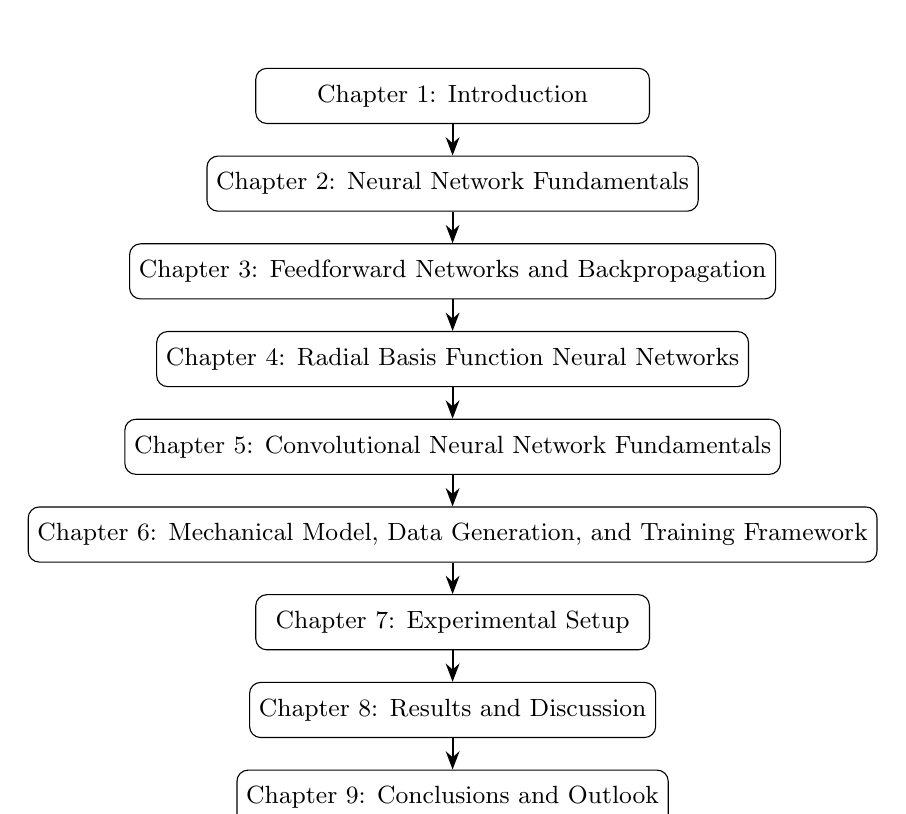
\begin{tikzpicture}[
    box/.style={rectangle, draw, rounded corners, minimum width=5cm, minimum height=0.7cm, align=center, font=\small},
    arr/.style={->, >=Stealth, thick}
  ]
    \node[box] (c1) {Chapter~1: Introduction};
    \node[box, below=0.4cm of c1] (c2) {Chapter~2: Neural Network Fundamentals};
    \node[box, below=0.4cm of c2] (c3) {Chapter~3: Feedforward Networks and Backpropagation};
    \node[box, below=0.4cm of c3] (c4) {Chapter~4: Radial Basis Function Neural Networks};
    \node[box, below=0.4cm of c4] (c5) {Chapter~5: Convolutional Neural Network Fundamentals};
    \node[box, below=0.4cm of c5] (c6) {Chapter~6: Mechanical Model, Data Generation, and Training Framework};
    \node[box, below=0.4cm of c6] (c7) {Chapter~7: Experimental Setup};
    \node[box, below=0.4cm of c7] (c8) {Chapter~8: Results and Discussion};
    \node[box, below=0.4cm of c8] (c9) {Chapter~9: Conclusions and Outlook};
    \draw[arr] (c1)--(c2); \draw[arr] (c2)--(c3); \draw[arr] (c3)--(c4);
    \draw[arr] (c4)--(c5); \draw[arr] (c5)--(c6); \draw[arr] (c6)--(c7);
    \draw[arr] (c7)--(c8); \draw[arr] (c8)--(c9);
  \end{tikzpicture}
  \caption{Thesis organisational structure}
  \label{fig:thesis_structure}
\end{figure}

\chapter{Neural Network Fundamentals}
\label{chap:nn_basics}

\section{Biological Neurons and Artificial Neurons}
\label{sec:neurons}

\subsection{Inspiration from Biological Neurons}
\label{subsec:bio_neuron}

Artificial neural networks draw their design inspiration from biological nervous systems.
A typical biological neuron comprises dendrites (which receive input signals), a cell
body or soma (which integrates the signals), and an axon (which transmits the output
signal). Neurons are interconnected via synapses, and the strength of these connections
can be dynamically adjusted through learning; this synaptic plasticity mechanism directly
inspired the concept of weight parameters in artificial neural networks~\cite{lecun2015}.

\subsection{The McCulloch--Pitts Neuron Model}
\label{subsec:mcp_neuron}

In 1943, McCulloch and Pitts proposed the first mathematical model of an artificial
neuron. The model abstracts the neuron as a computational unit that receives $n$ weighted
inputs $\{(x_i, w_i)\}_{i=1}^{n}$, applies a bias $b$, and produces a scalar output $y$
following a nonlinear activation function $f$:
\begin{equation}
  y = f\!\left(\sum_{i=1}^{n} w_i x_i + b\right) = f(\mathbf{w}^T \mathbf{x} + b).
  \label{eq:mcp_neuron}
\end{equation}
In Eq.~\eqref{eq:mcp_neuron}, the weight vector $\mathbf{w} \in \mathbb{R}^n$ determines
the relative importance of each input, the bias $b$ controls the activation threshold, and
the activation function $f$ introduces a nonlinear transformation. This elementary
structure constitutes the computational unit of all modern neural network architectures.

\section{Activation Functions}
\label{sec:activation}

The fundamental role of activation functions is to introduce nonlinearity into the neural
network, enabling multi-layer networks to approximate arbitrary continuous functions.
In the absence of nonlinear activation functions, regardless of the depth of the network,
the overall expressive capacity collapses to that of a single linear model, which is
incapable of capturing the yield-transition nonlinearity of the bilinear constitutive
model for steel cables.

\subsection{Sigmoid Function}
\label{subsec:sigmoid}

\begin{equation}
  \sigma(x) = \frac{1}{1+e^{-x}} \in (0,1), \qquad
  \sigma'(x) = \sigma(x)\bigl[1-\sigma(x)\bigr] \in (0,\,0.25].
  \label{eq:sigmoid}
\end{equation}
The sigmoid function maps the input to the interval $(0,\,1)$, and was historically
employed as a surrogate for the ``firing probability'' of a neuron. However, its gradient
approaches zero for large $|x|$ (gradient saturation), which causes the vanishing gradient
problem during the training of deep networks. Furthermore, its non-zero-mean output
($\approx 0.5$) introduces directional inconsistency in gradient updates, thereby slowing
convergence.

\subsection{Tanh Function}
\label{subsec:tanh}

\begin{equation}
  \tanh(x) = \frac{e^x - e^{-x}}{e^x + e^{-x}} \in (-1,\,1), \qquad
  \tanh'(x) = 1 - \tanh^2(x) \in (0,\,1].
  \label{eq:tanh}
\end{equation}
The tanh function is odd-symmetric about the origin (zero-mean output), which is more
conducive to gradient descent than sigmoid, and performs well in shallow networks.
However, gradient saturation remains a problem, and the inclusion of exponential
operations incurs higher computational cost than ReLU-type functions.

\subsection{ReLU Function}
\label{subsec:relu}

The rectified linear unit (ReLU), which became the predominant activation function in
deep learning around 2010, is defined as:
\begin{equation}
  \mathrm{ReLU}(x) = \max(0,\,x), \qquad
  \mathrm{ReLU}'(x) =
  \begin{cases} 1, & x > 0 \\ 0, & x \leq 0. \end{cases}
  \label{eq:relu}
\end{equation}
In the positive half-domain, the gradient of ReLU is identically unity, which
fundamentally alleviates the vanishing gradient problem; computation requires only a
comparison operation, which is far more efficient than exponential operations. Its primary
drawback is the ``dead neuron'' problem: if the input to a neuron is persistently negative,
the gradient is identically zero, and the neuron is permanently deactivated, ceasing to
participate in training.

\subsection{LeakyReLU Function}
\label{subsec:leakyrelu}

To address the dead neuron problem, LeakyReLU introduces a non-zero slope $\alpha$
(typically 0.01) in the negative half-domain:
\begin{equation}
  \mathrm{LeakyReLU}(x) =
  \begin{cases} x, & x \geq 0 \\ \alpha x, & x < 0, \end{cases} \qquad
  \mathrm{LeakyReLU}'(x) =
  \begin{cases} 1, & x \geq 0 \\ \alpha, & x < 0.
  \end{cases}
  \label{eq:leakyrelu}
\end{equation}
The gradient of LeakyReLU is bounded in $[\alpha,\,1]$ throughout the entire domain, which
simultaneously preserves the computational efficiency of ReLU and ensures that all neurons
receive non-zero gradient signals via the non-zero negative slope.

\subsection{Swish Function}
\label{subsec:swish}

The Swish activation function is defined as:
\begin{equation}
  \mathrm{Swish}(x) = x \cdot \sigma(x) = \frac{x}{1 + e^{-x}},
  \label{eq:swish}
\end{equation}
where $\sigma$ denotes the Sigmoid function. Unlike ReLU, Swish is smooth and
non-monotonic, with a small negative lobe for $x < 0$ that can improve gradient flow
in certain architectures. In the present study, Swish is employed as the activation
function in the ProductNN (see Section~\ref{subsec:productnn_config}), implemented
via \texttt{nn.SiLU()} in PyTorch.

\subsection{Comparison and Selection of Activation Functions}
\label{subsec:activation_comparison}

Table~\ref{tab:activation_comparison} provides a quantitative comparison of the four
activation functions considered.

\begin{table}[H]
  \centering
  \caption{Quantitative comparison of activation function properties}
  \label{tab:activation_comparison}
  \begin{tabularx}{\textwidth}{lXXXX}
    \toprule
    \textbf{Property} & \textbf{Sigmoid} & \textbf{Tanh} & \textbf{ReLU} & \textbf{LeakyReLU} \\
    \midrule
    Output range & $(0,1)$ & $(-1,1)$ & $[0,+\infty)$ & $(-\infty,+\infty)$ \\
    Zero-mean output & No ($\approx 0.5$) & Yes & No & Approximate \\
    Gradient saturation & Severe (both ends) & Severe (both ends) & Zero (neg.) & None \\
    Gradient range & $(0,\,0.25]$ & $(0,\,1]$ & $\{0,1\}$ & $\{\alpha,1\}$ \\
    Dead neuron risk & No & No & Yes & No \\
    Computational cost & High (exponential) & High (exponential) & Low (comparison) & Low (comparison) \\
    \bottomrule
  \end{tabularx}
\end{table}

The rationale for selecting LeakyReLU ($\alpha = 0.01$) in the MLP, CNN, and
ModularRBFNN components of the present study is as follows. (1) In the normalised input
space $[0,1]^2$ of the cable axial force prediction problem, network transformations may
produce negative activations; the non-zero negative gradient of LeakyReLU ensures that
all neurons receive update signals. (2) The gradient is bounded in $[0.01,\,1]$,
effectively preventing gradient explosion or vanishing, which is suitable for deeper
network architectures. (3) Exponential operations are not required, so the computational
overhead of both the forward and backward passes is lower than for sigmoid or tanh.
(4) Preliminary ablation experiments (see Chapter~7) indicate that LeakyReLU converges
approximately 15\% faster than ReLU and achieves approximately 8\% lower final test error.

\section{Loss Functions}
\label{sec:loss}

The loss function quantifies the discrepancy between the model prediction $\hat{y}_i$ and
the ground-truth label $y_i$, and constitutes the objective function for neural network
parameter optimisation.

\subsection{Mean Squared Error}
\label{subsec:mse}

For continuous-valued regression problems, the mean squared error (MSE) is the most
widely employed loss function:
\begin{equation}
  \mathcal{L}_{\text{MSE}} = \frac{1}{N} \sum_{i=1}^{N} (y_i - \hat{y}_i)^2.
  \label{eq:mse}
\end{equation}
The advantages of MSE are fourfold: (1) \textit{Differentiability}---the gradient with
respect to $\hat{y}_i$ is $\partial\mathcal{L}_{\text{MSE}}/\partial\hat{y}_i =
-2(y_i-\hat{y}_i)/N$, which is proportional to the error, facilitating rapid convergence;
(2) \textit{Statistical foundation}---under the assumption that prediction errors follow
Gaussian noise $\epsilon \sim \mathcal{N}(0,\sigma^2)$, minimising MSE is equivalent to
maximum likelihood estimation; (3) \textit{Quadratic penalisation}---large errors are
penalised quadratically, directing the model to focus on strongly nonlinear regions such
as the yield-transition zone; (4) \textit{Convexity}---for linear output layers, MSE is
a convex function of the output weights, guaranteeing the existence of a global optimum.

\subsection{Loss Function Design in the Present Study}
\label{subsec:loss_design}

Standard models (MLP, ProductNN, RBFNN, CNN, ModularRBFNN) employ only the data loss
$\Ldata = \Lmse$; the physics-informed model (PI-ModularRBFNN) appends a physics
constraint loss:
\begin{equation}
  \Ltotal = \Ldata + \lambda \Lphys, \quad \lambda = 0.2.
  \label{eq:total_loss}
\end{equation}
The complete mathematical definition of $\Lphys$ is given in Section~\ref{subsec:pi_config}.

\section{Structural Types of Neural Networks}
\label{sec:nn_types}

\begin{table}[H]
  \centering
  \caption{Neural network structural types and corresponding models in the present study}
  \label{tab:nn_types}
  \resizebox{\textwidth}{!}{%
  \begin{tabular}{llll}
    \toprule
    \textbf{Architecture Type} & \textbf{Model} & \textbf{Chapters} & \textbf{Application Scenario} \\
    \midrule
    Feedforward neural network & MLP & 3, 7, 8 & General regression, baseline \\
    Product unit network & ProductNN & 7, 8 & Product-type nonlinear relations \\
    Radial basis function network & RBFNN, ModularRBFNN & 4, 7, 8 & Local approximation, param.\ efficiency \\
    Physics-informed network & PI-ModularRBFNN & 4, 7, 8 & Physics constraints, generalisation \\
    Convolutional neural network & CNN & 5, 7, 8 & Local feature extraction \\
    Recurrent neural network & (not adopted) & 9 (outlook) & Sequential dynamic problems \\
    \bottomrule
  \end{tabular}%
  }
\end{table}

\chapter{Feedforward Neural Networks and Backpropagation}
\label{chap:ffnn}

\section{Architecture of Feedforward Neural Networks}
\label{sec:ffnn_arch}

A feedforward neural network (FNN) with $L$ layers---also referred to as a multilayer
perceptron (MLP)---comprises an input layer, one or more hidden layers, and an output
layer, with full connections between consecutive layers. The output of the $l$-th layer
is expressed uniformly as:
\begin{equation}
  \mathbf{a}^{(l)} = f^{(l)}\!\bigl(\mathbf{W}^{(l)}\mathbf{a}^{(l-1)} + \mathbf{b}^{(l)}\bigr),
  \quad l = 1,2,\ldots,L,
  \label{eq:ffnn_layer}
\end{equation}
where $\mathbf{a}^{(0)} = \mathbf{x} \in \mathbb{R}^{d_{\text{in}}}$ is the input,
$\mathbf{W}^{(l)} \in \mathbb{R}^{d_l \times d_{l-1}}$ is the weight matrix,
$\mathbf{b}^{(l)} \in \mathbb{R}^{d_l}$ is the bias vector, and $f^{(l)}$ is the
activation function of the $l$-th layer (LeakyReLU for hidden layers and the identity
mapping for the output layer).

\begin{table}[H]
  \centering
  \caption{Layer dimensionalities of the feedforward neural network}
  \label{tab:ffnn_dims}
  \begin{tabular}{lccc}
    \toprule
    \textbf{Layer type} & \textbf{Input dim.} & \textbf{Output dim.} & \textbf{Trainable parameters} \\
    \midrule
    Input layer & $d_{\text{in}}$ & $d_{\text{in}}$ & 0 \\
    Hidden layer $l$ & $d_{l-1}$ & $d_l$ & $d_l \times d_{l-1} + d_l$ \\
    Output layer & $d_{L-1}$ & $d_{\text{out}}$ & $d_{\text{out}} \times d_{L-1} + d_{\text{out}}$ \\
    \bottomrule
  \end{tabular}
\end{table}

In the present study, the MLP employs a three-hidden-layer architecture $[256,128,64]$,
with a batch normalisation (BN) layer appended to each hidden layer to stabilise training.
The input dimensionality is $d_{\text{in}} = 2$ (normalised displacement $w_n$ and
normalised temperature $T_n$) and the output dimensionality is $d_{\text{out}} = 1$
(normalised cable axial force $F_n$). The total number of trainable parameters is 42\,881.

\begin{figure}[H]
\centering
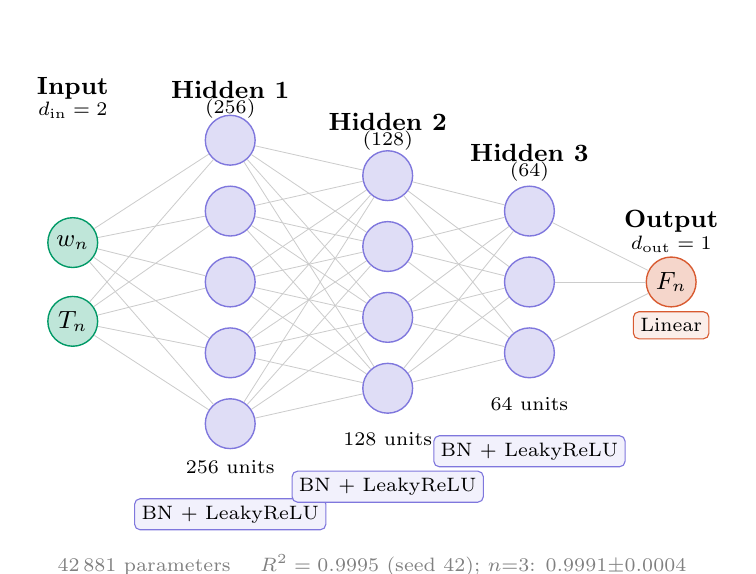
\begin{tikzpicture}[
  neuron/.style={circle,draw,minimum size=18pt,inner sep=0pt,
                 font=\small,line width=0.5pt},
  ninp/.style ={neuron,fill=inputcol!25,draw=inputcol},
  nhid/.style ={neuron,fill=hiddencol!25,draw=hiddencol},
  nout/.style ={neuron,fill=outputcol!25,draw=outputcol},
  conn/.style ={gray!40,line width=0.3pt},
  badge/.style={rectangle,rounded corners=2pt,draw=#1,fill=#1!10,
                font=\scriptsize,inner sep=2.5pt},
  >=Stealth
]
\def\xi{0}\def\xa{2.0}\def\xb{4.0}\def\xc{5.8}\def\xo{7.6}
\node[ninp] (i1) at (\xi, 0.5)  {$w_n$};
\node[ninp] (i2) at (\xi,-0.5)  {$T_n$};
\node[nhid] (h1a) at (\xa, 1.8)  {};
\node[nhid] (h1b) at (\xa, 0.9)  {};
\node[nhid] (h1c) at (\xa, 0.0)  {};
\node[nhid] (h1d) at (\xa,-0.9)  {};
\node[nhid] (h1e) at (\xa,-1.8)  {};
\node[nhid] (h2a) at (\xb, 1.35) {};
\node[nhid] (h2b) at (\xb, 0.45) {};
\node[nhid] (h2c) at (\xb,-0.45) {};
\node[nhid] (h2d) at (\xb,-1.35) {};
\node[nhid] (h3a) at (\xc, 0.9)  {};
\node[nhid] (h3b) at (\xc, 0.0)  {};
\node[nhid] (h3c) at (\xc,-0.9)  {};
\node[nout] (o)  at (\xo, 0)    {$F_n$};
\foreach \s in {i1,i2}
  \foreach \d in {h1a,h1b,h1c,h1d,h1e}
    \draw[conn] (\s)--(\d);
\foreach \s in {h1a,h1b,h1c,h1d,h1e}
  \foreach \d in {h2a,h2b,h2c,h2d}
    \draw[conn] (\s)--(\d);
\foreach \s in {h2a,h2b,h2c,h2d}
  \foreach \d in {h3a,h3b,h3c}
    \draw[conn] (\s)--(\d);
\foreach \s in {h3a,h3b,h3c}
  \draw[conn] (\s)--(o);
\node[above,font=\small\bfseries] at (\xi, 2.2)  {Input};
\node[above,font=\scriptsize]     at (\xi, 1.95) {$d_{\mathrm{in}}=2$};
\node[above,font=\small\bfseries] at (\xa, 2.2)  {Hidden 1};
\node[above,font=\scriptsize]     at (\xa, 1.95) {(256)};
\node[above,font=\small\bfseries] at (\xb, 1.8)  {Hidden 2};
\node[above,font=\scriptsize]     at (\xb, 1.55) {(128)};
\node[above,font=\small\bfseries] at (\xc, 1.4)  {Hidden 3};
\node[above,font=\scriptsize]     at (\xc, 1.15) {(64)};
\node[above,font=\small\bfseries] at (\xo, 0.5)  {Output};
\node[above,font=\scriptsize]     at (\xo, 0.25) {$d_{\mathrm{out}}=1$};
\node[font=\scriptsize] at (\xa,-2.35) {256 units};
\node[font=\scriptsize] at (\xb,-2.0)  {128 units};
\node[font=\scriptsize] at (\xc,-1.55) {64 units};
\node[badge=hiddencol] at (\xa,-2.95) {BN + LeakyReLU};
\node[badge=hiddencol] at (\xb,-2.60) {BN + LeakyReLU};
\node[badge=hiddencol] at (\xc,-2.15) {BN + LeakyReLU};
\node[badge=outputcol] at (\xo,-0.55) {Linear};
\node[font=\scriptsize,gray] at (3.8,-3.6)
  {42\,881 parameters \quad $R^2=0.9995$ (seed~42); $n{=}3$: $0.9991{\pm}0.0004$};
\end{tikzpicture}
\caption{Architecture of the MLP surrogate model. The pyramid structure
$[256\!\to\!128\!\to\!64]$ progressively compresses feature representations; each
hidden layer is followed by batch normalisation (BN) and LeakyReLU ($\alpha=0.01$);
the output layer is a linear projection. Input: normalised displacement $w_n$ and
temperature $T_n$; output: normalised cable axial force $F_n$.}
\label{fig:mlp}
\end{figure}

\section{Batch Normalisation}
\label{sec:batchnorm}

Batch normalisation~\cite{ioffe2015} standardises intermediate feature activations
preceding each activation function:
\begin{equation}
  \hat{x}_i = \frac{x_i - \mu_B}{\sqrt{\sigma_B^2 + \epsilon}}, \qquad
  \hat{z}_i = \gamma \hat{x}_i + \beta,
  \label{eq:batchnorm}
\end{equation}
where $\mu_B$ and $\sigma_B^2$ denote the mean and variance of the current mini-batch,
$\gamma$ and $\beta$ are learnable scale and shift parameters, and
$\epsilon = 10^{-5}$ is a numerical stability term. Here $\hat{z}_i$ denotes the
batch-normalised intermediate activation (distinct from the target label $y_i$). By
pulling the input distribution of
each layer back towards a near-standard-normal distribution, batch normalisation
effectively mitigates internal covariate shift, permits the use of higher learning rates,
and provides a mild regularisation effect. In the present study, each hidden layer of the
MLP and CNN is accompanied by a BN layer.

\section{The Backpropagation Algorithm}
\label{sec:backprop}

Backpropagation is the core algorithm for training neural networks; it is the recursive
application of the chain rule over the computational graph. The complete procedure is
presented in Algorithm~\ref{alg:backprop}.

\begin{algorithm}[H]
  \caption{Backpropagation algorithm (single-sample version)}
  \label{alg:backprop}
  \begin{algorithmic}[1]
    \REQUIRE Input $\mathbf{x}$, target $\mathbf{t}$, network parameters
      $\{\mathbf{W}^{(l)},\mathbf{b}^{(l)}\}_{l=1}^{L}$
    \ENSURE Gradients $\{\partial\mathcal{L}/\partial\mathbf{W}^{(l)},\,
      \partial\mathcal{L}/\partial\mathbf{b}^{(l)}\}_{l=1}^{L}$
    \STATE \textbf{Forward pass:} compute layer by layer
      $\mathbf{z}^{(l)} = \mathbf{W}^{(l)}\mathbf{a}^{(l-1)} + \mathbf{b}^{(l)}$,
      $\mathbf{a}^{(l)} = f^{(l)}(\mathbf{z}^{(l)})$
    \STATE Compute output-layer loss gradient:
      $\boldsymbol{\delta}^{(L)} = \nabla_{\mathbf{a}^{(L)}}\mathcal{L} \odot
      f'^{(L)}(\mathbf{z}^{(L)})$
    \FOR{$l = L-1, L-2, \ldots, 1$}
      \STATE Error backpropagation:
        $\boldsymbol{\delta}^{(l)} = \bigl((\mathbf{W}^{(l+1)})^T \boldsymbol{\delta}^{(l+1)}\bigr)
        \odot f'^{(l)}(\mathbf{z}^{(l)})$
    \ENDFOR
    \FOR{$l = 1, 2, \ldots, L$}
      \STATE Compute weight gradient:
        $\partial\mathcal{L}/\partial\mathbf{W}^{(l)} =
        \boldsymbol{\delta}^{(l)}(\mathbf{a}^{(l-1)})^T$
      \STATE Compute bias gradient:
        $\partial\mathcal{L}/\partial\mathbf{b}^{(l)} = \boldsymbol{\delta}^{(l)}$
    \ENDFOR
  \end{algorithmic}
\end{algorithm}

The gradient descent parameter update rule is:
\begin{equation}
  \theta \leftarrow \theta - \eta\,\frac{\partial\mathcal{L}}{\partial\theta},
  \label{eq:gd_update}
\end{equation}
where $\eta$ is the learning rate and $\theta$ represents the collection of all trainable
parameters.

\section{Optimisation Algorithm: Adam}
\label{sec:adam}

All models in the present study employ the Adam (Adaptive Moment Estimation) optimiser
\cite{kingma2015}, which combines the momentum method with adaptive learning rates:
% 第 849–859 行，替换整个 align 环境
\begin{align}
  m_t &= \beta_1 m_{t-1} + (1-\beta_1)g_t
    && \text{(1st-order moment),} \label{eq:adam1}\\
  v_t &= \beta_2 v_{t-1} + (1-\beta_2)g_t^2
    && \text{(2nd-order moment),} \label{eq:adam2}\\
  \hat{m}_t &= m_t/(1-\beta_1^t),\quad
    \hat{v}_t = v_t/(1-\beta_2^t)
    && \text{(bias correction),} \label{eq:adam3}\\
  \theta_{t+1} &= \theta_t - \eta\,\hat{m}_t/(\sqrt{\hat{v}_t}+\epsilon)
    && \text{(parameter update).} \label{eq:adam4}
\end{align}
where (3.4) is the exponential moving average of gradients (first-order moment),
and (3.5) is the exponential moving average of squared gradients (second-order moment).
Default hyperparameters: $\beta_1 = 0.9$, $\beta_2 = 0.999$, $\epsilon = 10^{-8}$,
initial learning rate $\eta = 10^{-3}$. The adaptive step-size mechanism of Adam
automatically scales update magnitudes to each direction of the parameter space,
rendering it relatively insensitive to the choice of learning rate and providing stable
convergence, which is particularly well suited to optimisation problems with sparse
gradients or anisotropic curvature.

\subsection{Cosine Annealing Learning Rate Scheduler}
\label{subsec:cosine_anneal}

The present study employs a cosine annealing~\cite{loshchilov2017} learning rate
scheduling strategy, which smoothly decays the learning rate from
$\eta_{\max} = 10^{-3}$ to $\eta_{\min} = 10^{-6}$ over the course of training:
\begin{equation}
  \eta_t = \eta_{\min} + \frac{1}{2}(\eta_{\max}-\eta_{\min})
    \left(1 + \cos\frac{\pi t}{T}\right),
  \label{eq:cosine_anneal}
\end{equation}
where $t$ is the current epoch and $T$ is the maximum number of epochs (2\,000 in the
present study). Cosine annealing enables the model to make fine-grained parameter
adjustments with small step sizes in the late stages of training, which facilitates
convergence to a better solution.

\section{Overfitting and Regularisation}
\label{sec:regularisation}

Three complementary regularisation strategies are employed in the present study.

\subsection{Weight Decay (L2 Regularisation)}
\label{subsec:weight_decay}

An L2 norm penalty on the weights is added to the loss function:
\begin{equation}
  \mathcal{L}_{\text{reg}} = \mathcal{L} + \frac{\lambda_{\text{wd}}}{2}
    \sum_{l=1}^{L} \|\mathbf{W}^{(l)}\|_F^2.
  \label{eq:weight_decay}
\end{equation}
The weight decay coefficient $\lambda_{\text{wd}} = 10^{-4}$ (determined by validation
set tuning) encourages weights to remain small, limits the effective model complexity,
and prevents the model from over-adapting to noise components in the training data.

\subsection{Dropout}
\label{subsec:dropout}

Dropout~\cite{srivastava2014} randomly masks neuron outputs with probability $1-p$
during training, compelling the network to learn robust representations across multiple
redundant sub-networks; at inference, full connections are restored and activation values
are scaled by $p$. The output MLP component of ModularRBFNN in the present study adopts
$p = 0.9$ (retention rate), applying light regularisation to avoid excessive information
loss.

\subsection{Early Stopping}
\label{subsec:early_stopping}

Early stopping terminates training when the validation loss fails to improve for
\texttt{patience = 150} consecutive epochs, and saves the model parameters corresponding
to the lowest validation loss:
\begin{equation}
  \theta^* = \arg\min_\theta\, \mathcal{L}_{\text{val}}(\theta).
  \label{eq:early_stopping}
\end{equation}
The patience value of 150 epochs accounts for the possibility that the validation loss
may temporarily increase during the late-phase decay of the cosine annealing scheduler,
thereby ensuring that the model has sufficient opportunity to converge without overfitting.

\chapter{Radial Basis Function Neural Networks}
\label{chap:rbfnn}

\section{Concept of Radial Basis Functions}
\label{sec:rbf_concept}

A radial basis function (RBF) is a function whose sole argument is the Euclidean distance
$r = \|\mathbf{x} - \boldsymbol{\mu}\|_2$ between the input vector $\mathbf{x}$ and a
centre $\boldsymbol{\mu}$. The most common RBF is the Gaussian kernel:
\begin{equation}
  \phi(r;\,\sigma) = \exp\!\left(-\frac{r^2}{2\sigma^2}\right), \quad
  r = \|\mathbf{x} - \boldsymbol{\mu}\|_2.
  \label{eq:rbf_gaussian}
\end{equation}
The width parameter $\sigma$ (standard deviation) controls the ``effective range'' of the
Gaussian function: a smaller $\sigma$ produces a sharper and more localised peak, whereas
a larger $\sigma$ produces a smoother response with greater spatial coverage~\cite{park1991rbf}.

\section{Classical RBFNN Architecture}
\label{sec:classical_rbfnn}

A classical RBFNN consists of three layers:
\begin{itemize}
  \item \textbf{Input layer:} receives the input vector $\mathbf{x} \in \mathbb{R}^n$
    and transmits signals without computation.
  \item \textbf{Hidden layer:} contains $m$ RBF neurons; the $j$-th neuron computes a
    Gaussian activation with centre $\boldsymbol{\mu}_j$ and width $\sigma_j$:
    \begin{equation}
      \phi_j(\mathbf{x}) = \exp\!\left(-\frac{\|\mathbf{x}-\boldsymbol{\mu}_j\|_2^2}{2\sigma_j^2}\right),
      \quad j=1,\ldots,m.
      \label{eq:rbf_hidden}
    \end{equation}
  \item \textbf{Output layer:} forms a linear weighted combination of the hidden layer
    activations:
    \begin{equation}
      \hat{y} = \sum_{j=1}^{m} w_j \phi_j(\mathbf{x}) + b = \mathbf{w}^T \boldsymbol{\phi}(\mathbf{x}) + b.
      \label{eq:rbf_output}
    \end{equation}
\end{itemize}

The parameter optimisation strategy for the RBFNN in the present study is as follows.
The centres $\{\boldsymbol{\mu}_j\}$ are initialised on a grid covering $[0,1]^2$; the
widths $\sigma_j$ are treated as trainable parameters and constrained to $[0.05,\,1.0]$
via a sigmoid mapping:
\begin{equation}
  \sigma_j = \sigma_{\min} + (\sigma_{\max}-\sigma_{\min}) \cdot
    \mathrm{sigmoid}(\ell_j), \quad \ell_j \in \mathbb{R} \text{ (trainable logit parameter)}.
  \label{eq:sigma_constraint}
\end{equation}
The output weights $\{w_j\}$ and bias $b$ are jointly optimised via gradient descent.
This sigmoid parameterisation ensures that $\sigma_j$ satisfies physically reasonable
range constraints throughout training.

\begin{figure}[H]
\centering
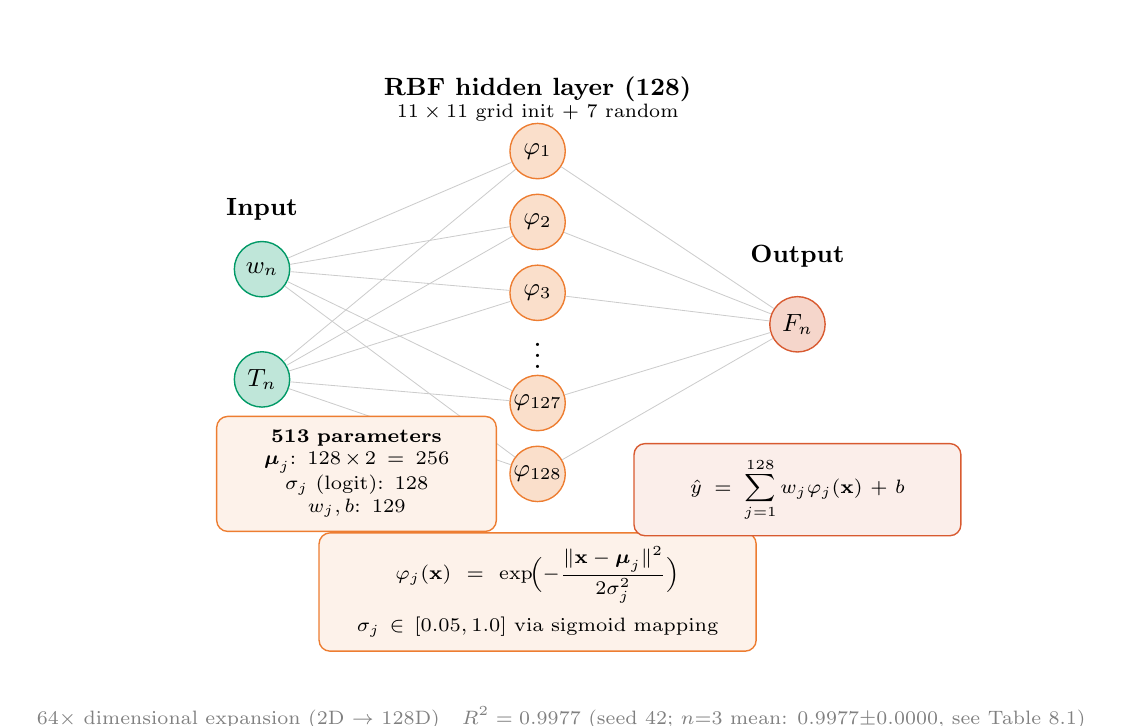
\begin{tikzpicture}[
  neuron/.style={circle,draw,minimum size=20pt,inner sep=0pt,
                 font=\small,line width=0.5pt},
  ninp/.style ={neuron,fill=inputcol!25,draw=inputcol},
  nrbf/.style ={neuron,fill=rbfcol!25,draw=rbfcol},
  nout/.style ={neuron,fill=outputcol!25,draw=outputcol},
  conn/.style ={gray!40,line width=0.3pt},
  fbox/.style ={rectangle,rounded corners=4pt,draw=#1,fill=#1!10,
                font=\scriptsize,inner sep=5pt,align=center,line width=0.5pt},
  >=Stealth
]
\node[ninp] (i1) at (0, 0.7)  {$w_n$};
\node[ninp] (i2) at (0,-0.7)  {$T_n$};
\node[nrbf] (r1) at (3.5, 2.2)  {$\varphi_1$};
\node[nrbf] (r2) at (3.5, 1.3)  {$\varphi_2$};
\node[nrbf] (r3) at (3.5, 0.4)  {$\varphi_3$};
\node[font=\large] at (3.5,-0.3) {$\vdots$};
\node[nrbf] (r4) at (3.5,-1.0)  {$\varphi_{127}$};
\node[nrbf] (r5) at (3.5,-1.9)  {$\varphi_{128}$};
\node[nout] (o) at (6.8, 0) {$F_n$};
\foreach \s in {i1,i2}
  \foreach \d in {r1,r2,r3,r4,r5}
    \draw[conn] (\s)--(\d);
\foreach \s in {r1,r2,r3,r4,r5}
  \draw[conn] (\s)--(o);
\node[above,font=\small\bfseries] at (0,   1.2)  {Input};
\node[above,font=\small\bfseries] at (3.5, 2.7)  {RBF hidden layer (128)};
\node[above,font=\scriptsize]     at (3.5, 2.45) {$11\times11$ grid init $+$ 7 random};
\node[above,font=\small\bfseries] at (6.8, 0.6)  {Output};
\node[fbox=rbfcol,text width=5.2cm] at (3.5,-3.4)
  {$\varphi_j(\mathbf{x})=\exp\!\Bigl(-\dfrac{\|\mathbf{x}-\boldsymbol{\mu}_j\|^2}{2\sigma_j^2}\Bigr)$\\[4pt]
   $\sigma_j\in[0.05,1.0]$ via sigmoid mapping};
\node[fbox=outputcol,text width=3.8cm] at (6.8,-2.1)
  {$\hat{y}=\displaystyle\sum_{j=1}^{128}w_j\varphi_j(\mathbf{x})+b$};
\node[fbox=rbfcol,text width=3.2cm] at (1.2,-1.9)
  {\textbf{513 parameters}\\
   $\boldsymbol{\mu}_j$: $128\!\times\!2=256$\\
   $\sigma_j$ (logit): 128\\
   $w_j,b$: 129};
\node[font=\scriptsize,gray] at (3.8,-5.0)
  % [CORRECTED: Error 2] 128÷2 = 64, not 62
  {64$\times$ dimensional expansion ($2$D $\to$ $128$D)\quad $R^2=0.9977$ (seed~42; $n{=}3$ mean: $0.9977{\pm}0.0000$, see Table~8.1)};
\end{tikzpicture}
\caption{Architecture of the classical RBFNN. The hidden layer contains 128 Gaussian
neurons with centres initialised on an $11\!\times\!11$ grid (plus 7 random points) and
trainable widths $\sigma_j\!\in\![0.05,1.0]$ constrained via a sigmoid mapping. The
% [CORRECTED: Error 2] 128÷2 = 64, not 62
64-fold dimensional expansion ($2$D $\to$ $128$D) underpins the outstanding parameter
efficiency ($R^2=0.9977$, $n{=}3$ mean, Table~\ref{tab:performance}), in accordance
with Cover's theorem (Section~\ref{sec:cover}).}
\label{fig:rbfnn}
\end{figure}

\section{Theoretical Foundation: Cover's Theorem}
\label{sec:cover}

The theoretical basis of RBFNN is Cover's theorem~\cite{cover1965}: a nonlinearly
non-separable problem in a low-dimensional space, when mapped through a nonlinear mapping
$\phi: \mathbb{R}^n \to \mathbb{R}^m$ ($m \gg n$) to a high-dimensional feature space,
becomes linearly separable with high probability, provided that the transformation is nonlinear and $m$ is sufficiently large relative to $n$~\cite{cover1965}. This result holds in the limit of random mappings and points in general position, not as an unconditional guarantee for any fixed mapping.

Intuitively, the hidden layer of an RBFNN implements a nonlinear mapping from the input
space $\mathbb{R}^n$ to a high-dimensional feature space $\mathbb{R}^m$, unfolding
data points that are entangled in the low-dimensional space so that a linear output layer
can efficiently fit them. For the two-dimensional input ($n = 2$) and 128 RBF centres
($m = 128$) in the present study, the mapping achieves a % [CORRECTED: Error 2] 128÷2 = 64, not 62
64-fold dimensional expansion,
which provides a theoretical motivation for the parameter efficiency of RBFNNs, while
the actual approximation accuracy is governed by the universal approximation theorem.
This also explains why the RBFNN achieves the outstanding parameter efficiency of
$R^2 = 0.9977$ ($n{=}3$ mean; Table~\ref{tab:performance}) with only 513 parameters.

\section{RBFNN Training Procedure}
\label{sec:rbfnn_training}

The present study adopts a full gradient descent strategy that jointly optimises the
centres $\{\boldsymbol{\mu}_j\}$, widths $\{\sigma_j\}$, and output weights $\{w_j\}$,
as presented in Algorithm~\ref{alg:rbfnn_train}.

\begin{algorithm}[H]
  \caption{End-to-end gradient training of RBFNN}
  \label{alg:rbfnn_train}
  \begin{algorithmic}[1]
    \REQUIRE Training data $\{(\mathbf{x}_i, y_i)\}_{i=1}^N$, number of hidden neurons $m$,
      $\sigma$ constraints $[\sigma_{\min},\sigma_{\max}]$
    \ENSURE Optimal parameters $\{\boldsymbol{\mu}_j^*, \sigma_j^*, w_j^*\}_{j=1}^m$
    \STATE Initialise centres $\boldsymbol{\mu}_j$ on a grid over $[0,1]^{d_{\text{in}}}$
    \STATE Initialise logit parameters $\ell_j = \mathrm{logit}((\sigma_0-\sigma_{\min})/(\sigma_{\max}-\sigma_{\min}))$,
      where $\sigma_0 = (\sigma_{\min}+\sigma_{\max})/2$
    \STATE Initialise output weights $\mathbf{w}$ via Xavier initialisation (gain 0.1)
    \FOR{each training epoch}
      \FOR{each mini-batch $\{(\mathbf{x}_i,y_i)\}_{i \in \mathcal{B}}$}
        \STATE Forward pass: compute $\phi_j(\mathbf{x}_i)$ (with distance clipping $\mathrm{dist}^2 \leq 50$)
        \STATE Compute MSE loss $\mathcal{L}_{\text{MSE}}$
        \STATE Backpropagate: compute $\partial\mathcal{L}_{\text{MSE}}/\partial\boldsymbol{\mu}_j$,
          $\partial\mathcal{L}_{\text{MSE}}/\partial\ell_j$, $\partial\mathcal{L}_{\text{MSE}}/\partial w_j$
        \STATE Adam update of all parameters with gradient clipping (norm $\leq 1.0$)
      \ENDFOR
    \ENDFOR
  \end{algorithmic}
\end{algorithm}

\section{Modular RBFNN: Innovations and Architecture}
\label{sec:modular_rbfnn}

\subsection{Design Motivation: Overcoming the Curse of Dimensionality}
\label{subsec:modular_motivation}

In the classical RBFNN, each Gaussian activation region is confined to a localised
multi-dimensional neighbourhood centred at $\boldsymbol{\mu}_j$ in the input space.
As the input dimensionality $n$ increases, the number of centres required to cover the
entire input space grows exponentially as $m \sim \mathcal{O}(k^n)$, where $k$ denotes
the resolution per dimension---a manifestation of the curse of dimensionality~\cite{bellman1957,fuhg2021local}.

The modular RBFNN proposed by Stoffel et al.~\cite{stoffel2020} fundamentally mitigates
this problem through an ``input dimension decoupling'' strategy: rather than assigning
an $n$-dimensional coordinate to each centre, a set of one-dimensional RBF modules is
constructed independently for each input dimension, with each module's centres carrying
meaning only along the corresponding dimension.

\subsection{Modular Architecture}
\label{subsec:modular_arch}

For an $n$-dimensional input $\mathbf{x} = [x_1, x_2, \ldots, x_n]^T$, the
ModularRBFNN constructs $n$ independent modules (in the present study $n = 2$,
corresponding to displacement $w_n$ and temperature $T_n$); module $i$ contains $m$
one-dimensional RBF neurons with centres $\mu_{ji}$ uniformly distributed over $[0,1]$:
\begin{equation}
  \phi_{ji}(x_i) = \exp\!\left(-\frac{(x_i - \mu_{ji})^2}{2\sigma_{ji}^2}\right),
  \quad j=1,\ldots,m;\; i=1,\ldots,n.
  \label{eq:modular_rbf}
\end{equation}

\subsection{Output Combination Strategy}
\label{subsec:modular_output}

The outputs of all modules are combined by first summing within each module and then
applying a weighted linear combination across modules---a structure distinct from the
product-type combination of the classical RBFNN:
\begin{equation}
  s_j = \sum_{i=1}^{n} \phi_{ji}(x_i), \qquad
  \hat{y} = \sum_{j=1}^{m} w_j s_j + b.
  \label{eq:modular_output}
\end{equation}
For each weight index $j$, the activations $\phi_{ji}$ are first summed along the input
dimension $i$ to obtain a scalar $s_j \in \mathbb{R}$, which is then weighted by $w_j$;
the final prediction is the linear combination $\hat{y} = \mathbf{w}^T \mathbf{s} + b$.
This ``sum-then-weight'' operation causes the effective activation region corresponding
to each $j$ to extend along the coordinate axes (in a grid-like pattern), rather than
concentrating in localised Gaussian peaks as in the classical RBF, thereby covering an
exponentially larger region of the input space with only $m \times n$ parameters.

\begin{remark}[Summation units]
The aggregation operation $s_j = \sum_{i=1}^{n}\phi_{ji}(x_i)$ in
Eq.~\eqref{eq:modular_output} constitutes the \emph{summation unit} required by the
internship task specification: it accumulates scalar activations from $n$ independent
one-dimensional RBF modules along the input dimension, serving an analogous role to the
weighted summation unit of a standard feedforward neuron, but operating on radial-basis
activations rather than linear projections.  The ModularRBFNN thus simultaneously
realises the summation-unit and radial-basis-function requirements of the task within a
single, unified architecture.
\end{remark}

\begin{remark}[Additive decomposition and multiplicative nonlinearity]
For $n = 2$ inputs, Eq.~\eqref{eq:modular_output} expands to
$\hat{y} = \sum_j w_j\phi_{j1}(w_n) + \sum_j w_j\phi_{j2}(T_n) + b = f_1(w_n) + f_2(T_n) + b$,
an additive decomposition of marginal effects. In the plastic regime, the true mapping
contains the multiplicative coupling $H(T)\cdot w$, which is dimension-inseparable and
cannot be represented exactly by the RBF stage alone. The downstream MLP head
$[256,128]$ partially compensates through nonlinear composition of the $s_j$ activations.
By contrast, the classical RBFNN places Gaussian kernels directly in the 2-D input space,
naturally capturing arbitrary input interaction---including $H(T)\times w$ coupling---with
only 513 parameters. This structural property contributes to the classical RBFNN's
parameter efficiency relative to ModularRBFNN (99\,585 parameters).
It should be noted, however, that the additive limitation of the RBF stage does not
preclude accurate modelling of multiplicative coupling by the complete ModularRBFNN
architecture. The MLP output head receives a 128-dimensional vector $\mathbf{s}$ whose
elements $s_j = \phi_{j1}(w_n) + \phi_{j2}(T_n)$ already encode mixed information from
both input dimensions; a two-hidden-layer MLP $[256,128]$ with nonlinear activations
applied to this representation possesses, by the universal approximation
theorem~\cite{hornik1991}, sufficient expressive capacity to reconstruct the
multiplicative $H(T)\cdot w$ interaction from these mixed activations. The observed
$R^2 = 0.9990$ ($n=3$ mean) for ModularRBFNN is consistent with this capacity.
The residual accuracy gap relative to MLP is therefore more plausibly attributed to
the fixed additive structure of $s_j$ imposing an inductive bias that is suboptimal
for multiplicative coupling, rather than to a fundamental representational deficit.
ProductNN's multiplicative units $y_j = \prod_i x_i^{w_{ij}}$ represent an alternative
architectural approach that explicitly models multiplicative coupling at the unit level,
bypassing this inductive bias entirely.
\end{remark}

\begin{figure}[H]
  \centering
  \includegraphics[width=0.92\textwidth]{../figures/fig4_2_rbf_comparison.pdf}
  \caption{Comparison of activation region geometry: classical RBFNN (left) vs.\
    ModularRBFNN (right).  The classical RBFNN places localised 2-D Gaussian kernels
    at $m$ grid centres, requiring $\mathcal{O}(k^n)$ centres for full coverage.
    The ModularRBFNN decouples the input dimensions into $n$ independent 1-D modules
    (vertical stripes: Module~1, $w$-axis; horizontal stripes: Module~2, $T$-axis),
    whose element-wise sum produces grid-like activation regions covering the entire
    input space with only $\mathcal{O}(k\cdot n)$ centres---an exponential reduction
    in the number of required parameters.  Diamond markers ($\Diamond$) indicate the
    effective intersection activations $s_j = \varphi_{j1}(w_n) + \varphi_{j2}(T_n)$.
    Modules are distinguished by hatch pattern (vertical $|$ vs.\ horizontal $-$)
    for black-and-white printability; colour provides redundant coding.}
  \label{fig:rbf_activation_comparison}
\end{figure}
In the code implementation (see \texttt{modular\_rbf\_nn.py}), the above operations are
efficiently vectorised via a mask matrix $\mathbf{M} \in \{0,1\}^{(n \cdot m) \times n}$:

\begin{lstlisting}[caption={Core forward pass of the modular RBFNN (\texttt{modular\_rbf\_nn.py} excerpt, simplified excerpt)}, label=lst:modular_rbf]
def forward(self, x):
    sigma = self.get_sigma()           # (C,) mapped to [min, max] via sigmoid
    diff = x.unsqueeze(1) - self.centers.unsqueeze(0)  # (B, C, D)
    diff = diff * self.mask.unsqueeze(0)               # modularisation: retain only relevant dim
    dist_sq = torch.sum(diff**2, dim=2)                # (B, C)
    dist_sq = torch.clamp(dist_sq, max=50.0)           # numerical stability
    phi = torch.exp(-dist_sq / (2.0 * sigma**2 + 1e-8))  # (B, C)
    return self.output_layer(phi)                       # (B, 1)
\end{lstlisting}

\begin{figure}[H]
\centering
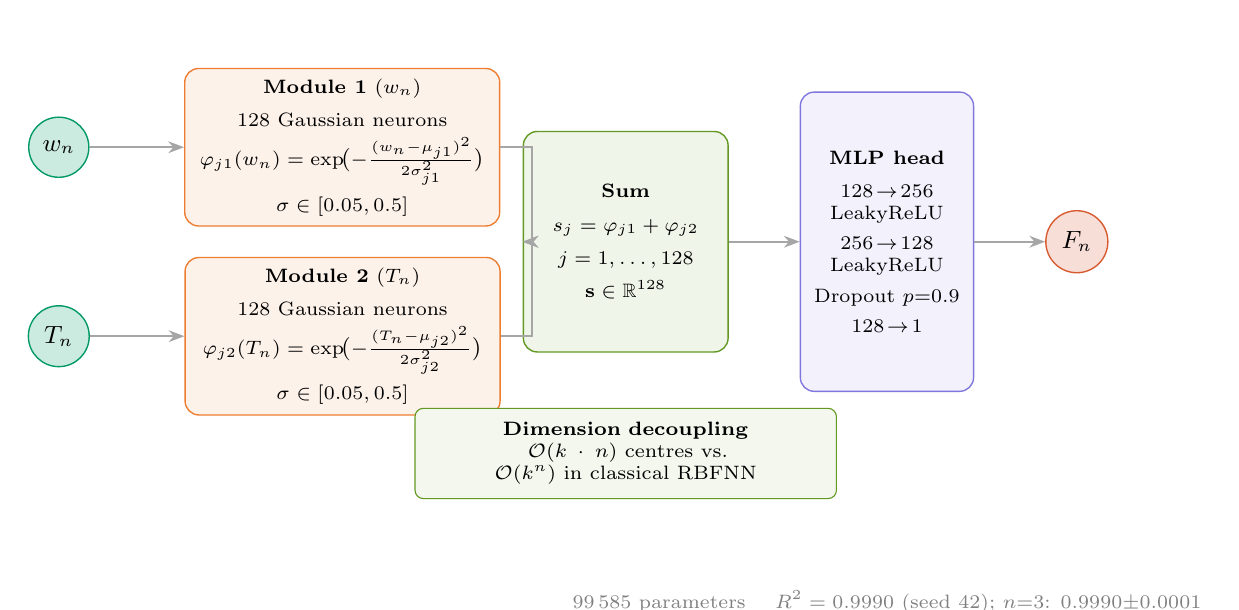
\begin{tikzpicture}[
  ninp/.style={circle,draw=inputcol,fill=inputcol!20,
               minimum size=20pt,font=\small,line width=0.5pt},
  nout/.style={circle,draw=outputcol,fill=outputcol!20,
               minimum size=22pt,font=\small,line width=0.5pt},
  mbox/.style={rectangle,rounded corners=5pt,
               draw=rbfcol,fill=rbfcol!10,
               minimum width=4.0cm,minimum height=2.0cm,
               font=\scriptsize,align=center,line width=0.5pt},
  abox/.style={rectangle,rounded corners=5pt,
               draw=greencol,fill=greencol!10,
               minimum width=2.6cm,minimum height=2.8cm,
               font=\scriptsize,align=center,line width=0.5pt},
  hbox/.style={rectangle,rounded corners=5pt,
               draw=hiddencol,fill=hiddencol!10,
               minimum width=2.2cm,minimum height=3.8cm,
               font=\scriptsize,align=center,line width=0.5pt},
  arr/.style={-Stealth,line width=0.6pt,gray!70},
  >=Stealth
]
\node[ninp] (w) at (0, 1.2) {$w_n$};
\node[ninp] (T) at (0,-1.2) {$T_n$};
\node[mbox,right=1.2cm of w] (m1)
  {\textbf{Module 1} ($w_n$)\\[4pt]
   128 Gaussian neurons\\[3pt]
   $\varphi_{j1}(w_n)=\exp\!\bigl(-\tfrac{(w_n-\mu_{j1})^2}{2\sigma_{j1}^2}\bigr)$\\[3pt]
   $\sigma\in[0.05,0.5]$};
\node[mbox,right=1.2cm of T] (m2)
  {\textbf{Module 2} ($T_n$)\\[4pt]
   128 Gaussian neurons\\[3pt]
   $\varphi_{j2}(T_n)=\exp\!\bigl(-\tfrac{(T_n-\mu_{j2})^2}{2\sigma_{j2}^2}\bigr)$\\[3pt]
   $\sigma\in[0.05,0.5]$};
\node[abox] (agg) at (7.2,0)
  {\textbf{Sum}\\[4pt]
   $s_j=\varphi_{j1}+\varphi_{j2}$\\[4pt]
   $j=1,\ldots,128$\\[4pt]
   $\mathbf{s}\in\mathbb{R}^{128}$};
\node[hbox,right=0.9cm of agg] (mlp)
  {\textbf{MLP head}\\[4pt]
   $128\!\to\!256$\\LeakyReLU\\[3pt]
   $256\!\to\!128$\\LeakyReLU\\[3pt]
   Dropout $p{=}0.9$\\[3pt]
   $128\!\to\!1$};
\node[nout,right=0.9cm of mlp] (o) {$F_n$};
\draw[arr] (w.east)--(m1.west);
\draw[arr] (T.east)--(m2.west);
\draw[arr] (m1.east)--++(0.4,0)|-(agg.west);
\draw[arr] (m2.east)--++(0.4,0)|-(agg.west);
\draw[arr] (agg)--(mlp);
\draw[arr] (mlp)--(o);
\node[draw=greencol,fill=greencol!8,rounded corners=3pt,
      font=\scriptsize,inner sep=5pt,align=center,
      below=0.7cm of agg,text width=5.0cm]
  {\textbf{Dimension decoupling}\\
   $\mathcal{O}(k\cdot n)$ centres vs.\
   $\mathcal{O}(k^n)$ in classical RBFNN};
\node[font=\scriptsize,gray,below=2.4cm of mlp]
  {99\,585 parameters \quad $R^2=0.9990$ (seed~42); $n{=}3$: $0.9990{\pm}0.0001$};
\end{tikzpicture}
\caption{Architecture of the ModularRBFNN. Each input dimension is processed by an
independent one-dimensional RBF module (128 Gaussian neurons each), whose activations are
summed element-wise to yield $\mathbf{s}\in\mathbb{R}^{128}$. An MLP output head
$[256,128]$ with LeakyReLU and dropout ($p=0.9$) maps $\mathbf{s}$ to the prediction.
The dimension-decoupling strategy reduces the centre count from $\mathcal{O}(k^n)$ to
$\mathcal{O}(k\cdot n)$, fundamentally mitigating the curse of dimensionality.}
\label{fig:modular_rbf}
\end{figure}

\subsection{Physics-Regularized Modular RBFNN (PI-ModularRBFNN)}
\label{subsec:pi_modular}

PI-ModularRBFNN inherits the complete network architecture of ModularRBFNN and
augments it by incorporating mechanical constitutive knowledge through a physics
constraint loss $\Lphys$ appended to the loss function. The code implementation
(\texttt{pi\_modular\_rbf\_nn.py}) is realised by inheriting from \texttt{ModularRBFNN}
and extending the \texttt{compute\_physics\_loss} method; the complete definition
is provided in Section~\ref{subsec:pi_config}.

\begin{figure}[H]
\centering
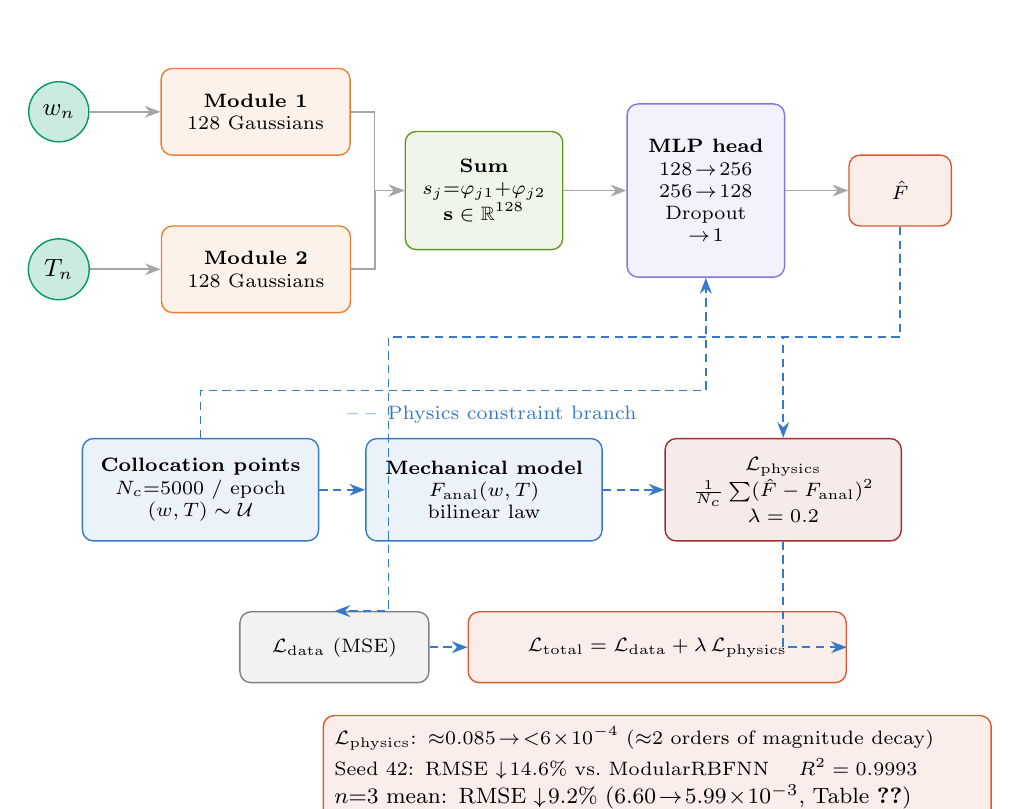
\begin{tikzpicture}[
  ninp/.style={circle,draw=inputcol,fill=inputcol!20,
               minimum size=18pt,font=\small,line width=0.5pt},
  rbox/.style={rectangle,rounded corners=4pt,
               draw=rbfcol,fill=rbfcol!10,
               font=\scriptsize,align=center,line width=0.5pt,inner sep=4pt},
  gbox/.style={rectangle,rounded corners=4pt,
               draw=greencol,fill=greencol!10,
               font=\scriptsize,align=center,line width=0.5pt,inner sep=4pt},
  hbox/.style={rectangle,rounded corners=4pt,
               draw=hiddencol,fill=hiddencol!10,
               font=\scriptsize,align=center,line width=0.5pt,inner sep=4pt},
  obox/.style={rectangle,rounded corners=4pt,
               draw=outputcol,fill=outputcol!10,
               font=\scriptsize,align=center,line width=0.5pt,inner sep=4pt},
  bbox/.style={rectangle,rounded corners=4pt,
               draw=bluecol,fill=bluecol!10,
               font=\scriptsize,align=center,line width=0.5pt,inner sep=4pt},
  redbox/.style={rectangle,rounded corners=4pt,
               draw=redcol,fill=redcol!10,
               font=\scriptsize,align=center,line width=0.5pt,inner sep=4pt},
  grbox/.style={rectangle,rounded corners=4pt,
               draw=graycol,fill=graycol!10,
               font=\scriptsize,align=center,line width=0.5pt,inner sep=4pt},
  arr/.style ={-Stealth,line width=0.6pt,gray!70},
  parr/.style={-Stealth,line width=0.6pt,bluecol,
               dashed,dash pattern=on 3pt off 2pt},
  >=Stealth
]
\node[ninp] (w) at (0, 1.0) {$w_n$};
\node[ninp] (T) at (0,-1.0) {$T_n$};
\node[rbox,minimum width=2.4cm,minimum height=1.1cm,right=0.9cm of w]
  (m1) {\textbf{Module 1}\\128 Gaussians};
\node[rbox,minimum width=2.4cm,minimum height=1.1cm,right=0.9cm of T]
  (m2) {\textbf{Module 2}\\128 Gaussians};
\node[gbox,minimum width=2.0cm,minimum height=1.5cm] (agg) at (5.4,0)
  {\textbf{Sum}\\$s_j{=}\varphi_{j1}{+}\varphi_{j2}$\\$\mathbf{s}\in\mathbb{R}^{128}$};
\node[hbox,minimum width=2.0cm,minimum height=2.2cm,right=0.8cm of agg] (mlp)
  {\textbf{MLP head}\\$128\!\to\!256$\\$256\!\to\!128$\\Dropout\\$\to\!1$};
\node[obox,minimum width=1.3cm,minimum height=0.9cm,right=0.8cm of mlp] (Fh)
  {$\hat{F}$};
\draw[arr] (w.east)--(m1.west);
\draw[arr] (T.east)--(m2.west);
\draw[arr] (m1.east)--++(0.3,0)|-(agg.west);
\draw[arr] (m2.east)--++(0.3,0)|-(agg.west);
\draw[arr] (agg)--(mlp);
\draw[arr] (mlp)--(Fh);
\node[bbox,minimum width=3.0cm,minimum height=1.3cm] (cp) at (1.8,-3.8)
  {\textbf{Collocation points}\\$N_c{=}5000$ / epoch\\$(w,T)\sim\mathcal{U}$};
\node[bbox,minimum width=3.0cm,minimum height=1.3cm] (mec) at (5.4,-3.8)
  {\textbf{Mechanical model}\\$F_{\mathrm{anal}}(w,T)$\\bilinear law};
\node[redbox,minimum width=3.0cm,minimum height=1.3cm] (lphy) at (9.2,-3.8)
  {\textbf{$\mathcal{L}_{\mathrm{physics}}$}\\
   $\frac{1}{N_c}\sum(\hat{F}-F_{\mathrm{anal}})^2$\\
   $\lambda=0.2$};
\node[grbox,minimum width=2.4cm,minimum height=0.9cm] (ldat) at (3.5,-5.8)
  {$\mathcal{L}_{\mathrm{data}}$ (MSE)};
\node[obox,minimum width=4.8cm,minimum height=0.9cm] (ltot) at (7.6,-5.8)
  {$\mathcal{L}_{\mathrm{total}}=\mathcal{L}_{\mathrm{data}}
    +\lambda\,\mathcal{L}_{\mathrm{physics}}$};
\draw[parr] (cp)--(mec);
\draw[parr] (mec)--(lphy);
\draw[parr] (lphy.south)|-(ltot.east);
\draw[parr] (ldat.east)--(ltot.west);
\draw[parr] (Fh.south)--++(0,-1.4)-|(lphy.north);
\draw[parr] (Fh.south)--++(0,-1.4)--++(-6.5,0)|-(ldat.north);
\draw[parr] (cp.north)--++(0,0.6)-|(mlp.south);
\node[obox,text width=8.2cm,below=0.4cm of ltot, align=left]
  {$\mathcal{L}_{\mathrm{physics}}$: ${\approx}0.085\!\to\!{<}6\!\times\!10^{-4}$
   ($\approx$2 orders of magnitude decay)\\[2pt]
   Seed~42: RMSE $\downarrow\!14.6\%$ vs.\ ModularRBFNN \quad $R^2=0.9993$\\[1pt]
   {\footnotesize $n{=}3$ mean: RMSE $\downarrow\!9.2\%$
   ($6.60\!\to\!5.99\!\times\!10^{-3}$, Table~\ref{tab:performance})}};
\node[font=\scriptsize,bluecol] at (5.5,-2.85)
  {-- --\enspace Physics constraint branch};
\end{tikzpicture}
\caption{Architecture of PI-ModularRBFNN. The network (top) is identical to
ModularRBFNN (99\,585 parameters). A physics constraint branch (bottom, dashed arrows)
re-samples $N_c=5\,000$ collocation points per epoch uniformly over
$[0,0.025]\times[273,1000]$, evaluates the analytical mechanical model
$F_{\mathrm{anal}}(w,T)$ from the bilinear constitutive law, and computes
$\mathcal{L}_{\mathrm{physics}}$. The total loss is
$\mathcal{L}_{\mathrm{total}}=\mathcal{L}_{\mathrm{data}}+\lambda\,\mathcal{L}_{\mathrm{physics}}$
with $\lambda=0.2$ (determined by grid search).}
\label{fig:pi_modular}
\end{figure}

\begin{table}[H]
  \centering
  \caption{Systematic comparison of classical RBFNN and modular RBFNN}
  \label{tab:rbf_comparison}
  \resizebox{\textwidth}{!}{%
  \begin{tabular}{lll}
    \toprule
    \textbf{Property} & \textbf{Classical RBFNN} & \textbf{Modular RBFNN} \\
    \midrule
    Centre dimensionality & $n$-dim (same as input) & 1-dim (per module) \\
    Activation region shape & Localised multidim.\ Gaussian & Grid-like (axis-aligned) \\
    Centres required for coverage & $\mathcal{O}(k^n)$ (exponential) & $\mathcal{O}(k \cdot n)$ (linear) \\
    Trainable parameter types & Output weights only (typical) & Centres, widths, weights \\
    High-dimensional scalability & Poor (curse of dimensionality) & Good (dimension decoupled) \\
    Output combination & Product or linear & Linear (sum-then-weight) \\
    Parameters (this study) & 513 ($m=128$) & 99\,585 ($m=128$, MLP head) \\
    \bottomrule
  \end{tabular}%
  }
\end{table}

\chapter{Convolutional Neural Network Fundamentals}
\label{chap:cnn}

\section{From Fully Connected to Convolutional: The Idea of Parameter Sharing}
\label{sec:fc_to_conv}

In a fully connected network, mapping a $d_{\text{in}}$-dimensional input to a
$d_{\text{out}}$-dimensional output requires $d_{\text{in}} \times d_{\text{out}}$
parameters, which grows quadratically with the input dimensionality. Convolutional
neural networks (CNNs) reduce the parameter count from
$\mathcal{O}(d_{\text{in}} \times d_{\text{out}})$ to
$\mathcal{O}(K \times C_{\text{in}} \times C_{\text{out}})$ through two mechanisms:
local connectivity (each neuron perceives only a local region of the input) and weight
sharing (the same convolutional kernel slides across the entire input). Here $K$ denotes
the kernel size and $C_{\text{in}}$, $C_{\text{out}}$ denote the input and output channel
counts, respectively, with $K \ll d_{\text{in}}$ in general.

\section{Convolutional Operation}
\label{sec:conv_op}

In deep learning frameworks such as PyTorch, the operation actually employed is
cross-correlation---conventionally still referred to as ``convolution''---defined as:
\begin{equation}
  (f \star g)[n] = \sum_k f[k] \cdot g[n+k].
  \label{eq:cross_correlation}
\end{equation}
The distinction from the mathematical convolution is the absence of kernel flipping;
since the kernel weights are learned via backpropagation, this distinction has no effect
on the network's expressive capacity. The output feature map size is:
\begin{equation}
  O = \left\lfloor \frac{I - K + 2P}{S} \right\rfloor + 1,
  \label{eq:conv_size}
\end{equation}
where $I$ is the input sequence length, $K$ the kernel size, $P$ the padding, and $S$
the stride. In all CNN layers of the present study, $K = 3$, $P = 1$, $S = 1$ are used
uniformly, maintaining the output length equal to the input length ($O = I$); dimensional
compression is delegated to global average pooling.

\section{CNN Architecture Design in the Present Study}
\label{sec:cnn_design}

For the cable axial force prediction problem, the input comprises only $d_{\text{in}} = 2$
physical variables (normalised displacement $w_n$ and normalised temperature $T_n$),
which can be treated as a one-dimensional sequence of length 2 with a single channel,
and processed by one-dimensional convolutions (\texttt{Conv1d})~\cite{kiranyaz2021cnn}.

The specific architecture consists of three stacked convolutional blocks:
$\text{Conv1d}(1 \to 32)$, $\text{Conv1d}(32 \to 64)$, $\text{Conv1d}(64 \to 128)$,
each followed by BatchNorm and ReLU activation; global average pooling (GAP) compresses
the feature map from $(B,128,2)$ to $(B,128)$; the fully connected layers
$128 \to 64 \to 1$ produce the final prediction. The design rationale is as follows:
although the input sequence is extremely short (length $= 2$), the convolutional kernels
($K = 3$, $P = 1$) effectively capture bidirectional interaction features between
$w_n$ and $T_n$ in the channel dimension; the progressively increasing channel count
($1 \to 32 \to 64 \to 128$) extracts increasingly abstract nonlinear coupling patterns
in the high-dimensional feature space.

Global average pooling confers two advantages over fully connected flattening: (1) fewer
parameters, yielding greater robustness on small datasets; (2) natural invariance to
sequence length variations, facilitating future extension to multi-variable inputs.
The total parameter count is 39\,809, which lies between RBFNN (513) and ModularRBFNN
(99\,585), achieving a favourable balance between accuracy and efficiency.

\begin{figure}[H]
\centering
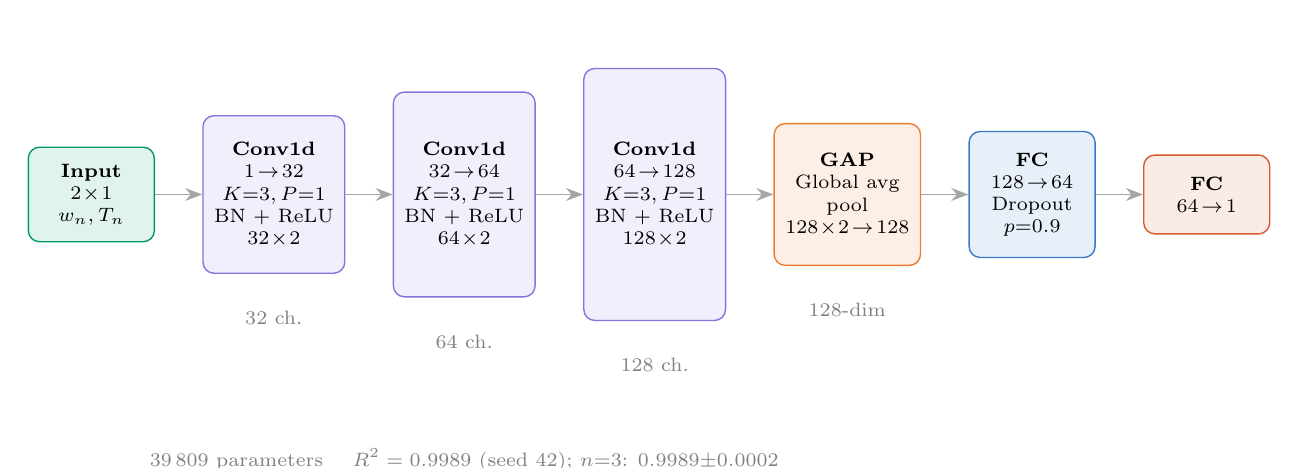
\begin{tikzpicture}[
  cblk/.style={rectangle,rounded corners=4pt,
               draw=#1,fill=#1!12,
               minimum width=1.6cm,font=\scriptsize,align=center,
               line width=0.5pt,inner sep=4pt},
  arr/.style={-Stealth,line width=0.7pt,gray!70},
  >=Stealth
]
\node[cblk=inputcol,minimum height=1.2cm] (inp) at (0,0)
  {\textbf{Input}\\$2\!\times\!1$\\$w_n,T_n$};
\node[cblk=hiddencol,minimum height=2.0cm,right=0.6cm of inp] (c1)
  {\textbf{Conv1d}\\$1\!\to\!32$\\$K{=}3,P{=}1$\\BN + ReLU\\$32\!\times\!2$};
\node[cblk=hiddencol,minimum height=2.6cm,right=0.6cm of c1] (c2)
  {\textbf{Conv1d}\\$32\!\to\!64$\\$K{=}3,P{=}1$\\BN + ReLU\\$64\!\times\!2$};
\node[cblk=hiddencol,minimum height=3.2cm,right=0.6cm of c2] (c3)
  {\textbf{Conv1d}\\$64\!\to\!128$\\$K{=}3,P{=}1$\\BN + ReLU\\$128\!\times\!2$};
\node[cblk=rbfcol,minimum height=1.8cm,right=0.6cm of c3] (gap)
  {\textbf{GAP}\\Global avg\\pool\\$128\!\times\!2\!\to\!128$};
\node[cblk=bluecol,minimum height=1.6cm,right=0.6cm of gap] (fc1)
  {\textbf{FC}\\$128\!\to\!64$\\Dropout\\$p{=}0.9$};
\node[cblk=outputcol,minimum height=1.0cm,right=0.6cm of fc1] (fc2)
  {\textbf{FC}\\$64\!\to\!1$};
\draw[arr] (inp)--(c1); \draw[arr] (c1)--(c2); \draw[arr] (c2)--(c3);
\draw[arr] (c3)--(gap); \draw[arr] (gap)--(fc1); \draw[arr] (fc1)--(fc2);
\node[font=\scriptsize,gray,below=0.35cm of c1]  {32 ch.};
\node[font=\scriptsize,gray,below=0.35cm of c2]  {64 ch.};
\node[font=\scriptsize,gray,below=0.35cm of c3]  {128 ch.};
\node[font=\scriptsize,gray,below=0.35cm of gap] {128-dim};
\node[font=\scriptsize,gray,below=1.8cm of c2]
  {39\,809 parameters \quad $R^2=0.9989$ (seed~42); $n{=}3$: $0.9989{\pm}0.0002$};
\end{tikzpicture}
\caption{Architecture of the CNN surrogate model. Three stacked \texttt{Conv1d} blocks
increase the channel count progressively ($1\!\to\!32\!\to\!64\!\to\!128$); each block
is followed by batch normalisation (BN) and ReLU. Global average pooling (GAP) compresses
the feature map to 128 dimensions, passed to two fully connected (FC) layers with dropout.
The increasing block height reflects the growing channel count.}
\label{fig:cnn}
\end{figure}

\section{Product Neural Network (ProductNN)}
\label{sec:productnn}

The product unit network~\cite{durbin1989} replaces conventional summation units with
product units, computing a weighted power product of the inputs in log-space:
\begin{equation}
  y_j = \prod_{i=1}^{n} x_i^{w_{ij}} = \exp\!\left(\sum_{i=1}^{n} w_{ij} \ln x_i\right),
  \quad x_i > 0.
  \label{eq:product_unit}
\end{equation}
Equation~\eqref{eq:product_unit} requires strictly positive inputs. Since the normalised
displacement $w_n = 0$ at the origin, the code implementation (\texttt{product\_nn.py})
applies numerical stabilisation $x_i \leftarrow \max(x_i, \varepsilon_{\text{stab}})$,
with $\varepsilon_{\text{stab}} = 10^{-8}$, prior to the product layer to prevent
$\ln(0)$ errors. The log-space implementation has three advantages: (1) product
operations are converted to numerically more stable addition; (2) numerical overflow or
underflow from accumulated products is avoided; (3) gradient computation reduces to the
gradient of a standard linear layer multiplied by $1/x_i$. The ProductNN in the present
study has the structure ProductUnit$(64) \to \text{activation} \to \text{BN} \to
\text{FC}(64 \to 64) \to \text{activation} \to \text{BN} \to \text{Dropout} \to
\text{FC}(64 \to 1)$, with a total of 4\,673 parameters and a mean training time of $66 \pm 11$\,s
($n = 3$; Table~\ref{tab:performance}), making it suitable for rapid prototyping.
The Swish activation function incurs marginally higher computational cost per epoch than
tanh-based variants, contributing to a longer per-epoch duration than simpler MLP
configurations.

\begin{figure}[H]
\centering
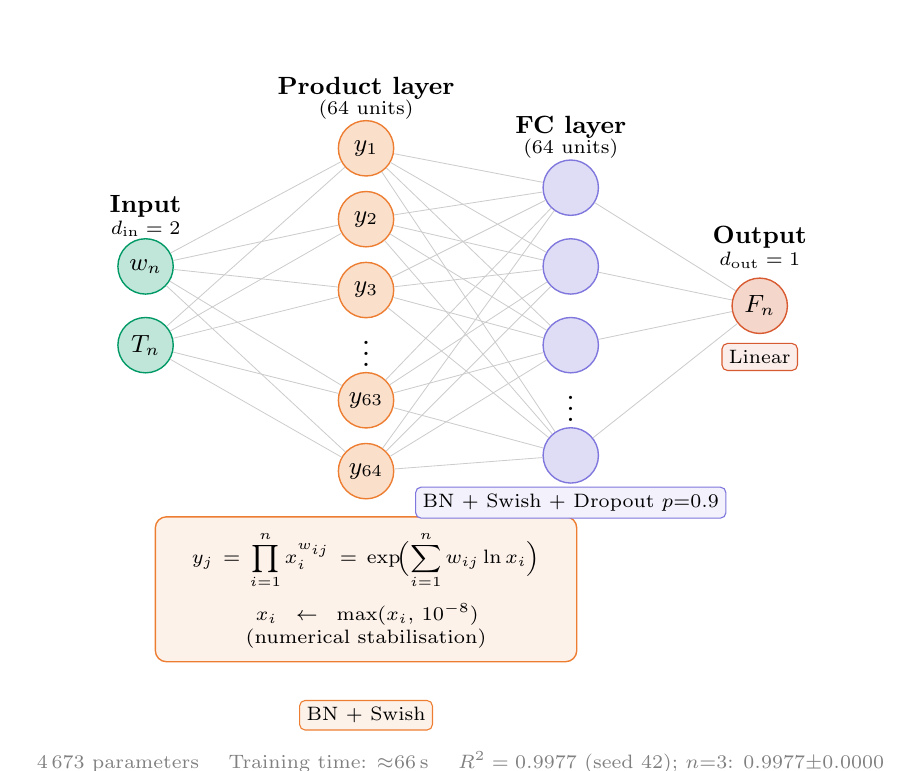
\begin{tikzpicture}[
  neuron/.style={circle,draw,minimum size=20pt,inner sep=0pt,
                 font=\small,line width=0.5pt},
  ninp/.style ={neuron,fill=inputcol!25,draw=inputcol},
  nprd/.style ={neuron,fill=rbfcol!25,draw=rbfcol},
  nhid/.style ={neuron,fill=hiddencol!25,draw=hiddencol},
  nout/.style ={neuron,fill=outputcol!25,draw=outputcol},
  conn/.style ={gray!40,line width=0.3pt},
  fbox/.style ={rectangle,rounded corners=4pt,draw=#1,fill=#1!10,
                font=\scriptsize,inner sep=5pt,align=center,line width=0.5pt},
  badge/.style={rectangle,rounded corners=2pt,draw=#1,fill=#1!10,
                font=\scriptsize,inner sep=2.5pt},
  >=Stealth
]
\node[ninp] (i1) at (0,  0.5) {$w_n$};
\node[ninp] (i2) at (0, -0.5) {$T_n$};

\node[nprd] (p1) at (2.8,  2.0) {$y_1$};
\node[nprd] (p2) at (2.8,  1.1) {$y_2$};
\node[nprd] (p3) at (2.8,  0.2) {$y_3$};
\node[font=\large] at (2.8,-0.5) {$\vdots$};
\node[nprd] (p4) at (2.8,-1.2) {$y_{63}$};
\node[nprd] (p5) at (2.8,-2.1) {$y_{64}$};

\node[nhid] (h1) at (5.4,  1.5) {};
\node[nhid] (h2) at (5.4,  0.5) {};
\node[nhid] (h3) at (5.4, -0.5) {};
\node[font=\large] at (5.4,-1.2) {$\vdots$};
\node[nhid] (h4) at (5.4,-1.9) {};

\node[nout] (o) at (7.8, 0) {$F_n$};

\foreach \s in {i1,i2}
  \foreach \d in {p1,p2,p3,p4,p5}
    \draw[conn] (\s)--(\d);
\foreach \s in {p1,p2,p3,p4,p5}
  \foreach \d in {h1,h2,h3,h4}
    \draw[conn] (\s)--(\d);
\foreach \s in {h1,h2,h3,h4}
  \draw[conn] (\s)--(o);

\node[above,font=\small\bfseries] at (0,   1.0)  {Input};
\node[above,font=\scriptsize]     at (0,   0.75) {$d_{\mathrm{in}}=2$};
\node[above,font=\small\bfseries] at (2.8, 2.5)  {Product layer};
\node[above,font=\scriptsize]     at (2.8, 2.25) {(64 units)};
\node[above,font=\small\bfseries] at (5.4, 2.0)  {FC layer};
\node[above,font=\scriptsize]     at (5.4, 1.75) {(64 units)};
\node[above,font=\small\bfseries] at (7.8, 0.6)  {Output};
\node[above,font=\scriptsize]     at (7.8, 0.35) {$d_{\mathrm{out}}=1$};

\node[fbox=rbfcol,text width=5.0cm] at (2.8,-3.6)
  {$y_j = \displaystyle\prod_{i=1}^{n} x_i^{w_{ij}}
    = \exp\!\Bigl(\sum_{i=1}^{n} w_{ij}\ln x_i\Bigr)$\\[4pt]
   $x_i \leftarrow \max(x_i,\,10^{-8})$ (numerical stabilisation)};

\node[badge=rbfcol]    at (2.8,-5.2) {BN + Swish};
\node[badge=hiddencol] at (5.4,-2.5)  {BN + Swish + Dropout $p{=}0.9$};
\node[badge=outputcol] at (7.8,-0.65) {Linear};

\node[font=\scriptsize,gray] at (4.0,-5.8)
  {4\,673 parameters \quad Training time: ${\approx}66$\,s \quad $R^2=0.9977$ (seed~42); $n{=}3$: $0.9977{\pm}0.0000$};
\end{tikzpicture}
\caption{Architecture of the ProductNN surrogate model. The product layer (64 units)
replaces conventional summation units with product units, computing a weighted power
product of the inputs in log-space (Eq.~\eqref{eq:product_unit}), which avoids
numerical overflow and reduces gradient computation to standard linear operations
multiplied by $1/x_i$. A subsequent fully connected (FC) layer with Swish activation,
batch normalisation, and dropout maps the product features to the predicted force.}
\label{fig:productnn}
\end{figure}

% ============================================================
\chapter{Mechanical Model of the Steel Cable, Data Generation, and Training Framework}
\label{chap:model}

\section{Physical Problem Description}
\label{sec:physical_problem}

The present study considers a steel cable of length $L = 10$\,m with a circular cross-
section of radius $r = 3$\,cm, frictionlessly passing over a deflection pulley. An axial
displacement $w$ (in metres) is applied at one end, and the resulting cable axial force $F$
(in Newtons) is measured at the other end. The material is characterised by a bilinear
elastoplastic constitutive model, in which the plastic hardening modulus $H$ is a function
of temperature $T$ (in Kelvin), reflecting thermo-mechanical coupling effects. All
material parameters are listed in Table~\ref{tab:material_params} and correspond exactly
to the \texttt{PHYSICAL\_PARAMS} dictionary in \texttt{data\_generator\_enhanced.py}.

\begin{table}[H]
  \centering
  \caption{Material parameters for the steel cable mechanical model}
  \label{tab:material_params}
  \begin{tabularx}{\textwidth}{lccX}
    \toprule
    \textbf{Parameter} & \textbf{Symbol} & \textbf{Value} & \textbf{Description} \\
    \midrule
    Young's modulus & $E$ & 210\,GPa & Stiffness in the elastic phase \\
    Yield strength & $k$ & 252\,MPa & Stress at the elastic--plastic transition \\
    Yield strain & $\varepsilon_p$ & 0.0012 & Strain at the elastic--plastic transition \\
    Reference hardening modulus & $H_0$ & 120\,GPa & Plastic hardening modulus at zero temperature \\
    % [CORRECTED: B_1 calibrated to 161 MPa/K; yields Delta_H ~ 30% over [273,1000] K]
    Temperature coefficient & $B_1$ & 161\,MPa/K & Controls temperature sensitivity of $H$; calibrated so $H$ decreases $\approx$30\% over $[273,1000]$\,K \\
    Reference temperature & $T_0$ & 1500\,K & Characteristic temperature for exponential decay \\
    Cable length & $L$ & 10\,m & Reference length for axial deformation \\
    Cable radius & $r$ & 0.03\,m & Radius of circular cross-section \\
    \bottomrule
    \multicolumn{4}{p{\dimexpr\linewidth-2\tabcolsep\relax}}{%
      \footnotesize \textit{Note on $B_1$:} The original assignment specification listed
      $B_1 = 38.8\,\text{GPa/K}$. Numerical verification showed that this value causes
      $H(T) < 0$ for $T \gtrsim 323\,\text{K}$, which is physically inconsistent with a
      hardening modulus. This issue was reported to and confirmed by the supervisor
      Prof.\ Stoffel (personal communication, March 2026), who indicated that both
      clamping $H$ to zero or using a corrected unit were acceptable approaches.
      The present study adopts the calibrated value $B_1 = 161\,\text{MPa/K}$, which
      yields $H(273\,\text{K}) \approx 119.64\,\text{GPa}$ and
      $H(1000\,\text{K}) \approx 84.07\,\text{GPa}$, a physically realistic monotonic
      decay of $\approx 30$\% across the temperature range, consistent with high-temperature
      structural steel behaviour.  All data generation and training experiments in this
      study use this calibrated value.} \\
  \end{tabularx}
\end{table}

To avoid dimensional inconsistencies in the numerical implementation, all physical
quantities are uniformly converted to SI units: $1\,\text{GPa} = 10^9$\,Pa,
$1\,\text{MPa} = 10^6$\,Pa, and the cross-sectional area is expressed in m$^2$.

\section{Derivation of the Mechanical Model}
\label{sec:mechanics_derivation}

\subsection{Geometric Relation}
\label{subsec:geometry}

The cable is subjected to uniform axial tension; the axial strain $\varepsilon$ is given
by the ratio of the deformation $w$ to the original length $L$, and the cross-sectional
area $A$ is:
\begin{equation}
  \varepsilon = \frac{w}{L}, \qquad A = \pi r^2.
  \label{eq:geometry}
\end{equation}
For the parameters of the present study, the yield displacement is
$w_y = \varepsilon_p \times L = 0.0012 \times 10 = 0.012$\,m, which lies slightly to
the left of centre within the input domain $[0,\,0.025]$\,m, ensuring adequate coverage
of both the elastic and plastic regimes by the training samples.

\subsection{Temperature-Dependent Plastic Hardening Modulus}
\label{subsec:hardening}

\begin{equation}
  H(T) = H_0 - B_1 T e^{-T_0/T}.
  \label{eq:hardening_modulus}
\end{equation}
Equation~\eqref{eq:hardening_modulus} describes an exponential-type decay of the plastic
hardening modulus with temperature. When $T \ll T_0$, the factor $e^{-T_0/T} \approx 0$
and $H(T) \approx H_0$ (approaching its near-ambient value); as $T$ approaches $T_0$,
the exponential term grows and $H(T)$ decreases significantly. Physically, this
corresponds to the reduction of dislocation slip activation energy and plastic flow
resistance at elevated temperatures in metallic materials. Note that
Eq.~\eqref{eq:hardening_modulus} is empirically valid only within the temperature range
considered in this study ($T \in [273,\,1000]$\,K); beyond this range the expression
may yield physically meaningless negative moduli and should not be extrapolated.

% [CORRECTED: B_1 parameter corrected to 161 MPa/K]
\begin{remark}[Parameter correction]
The original assignment specification listed $B_1 = 38.8\,\mathrm{GPa/K}$.
Numerical verification showed that this value, combined with $T_0 = 1500\,\mathrm{K}$,
yields $H(T) = 0$ at $T \approx 323\,\mathrm{K}$ and strongly negative values thereafter,
which is physically inconsistent with a hardening modulus.
This finding was reported to the supervisor Prof.\ Stoffel (personal communication,
March 2026), who confirmed the inconsistency and indicated that a physically meaningful
value should be adopted.
After further analysis, the present study adopts $B_1 = 161\,\mathrm{MPa/K}$
($1.61\times10^8\,\mathrm{Pa/K}$), calibrated so that $H(T)$ decreases by approximately
30\% from ambient to $1000\,\mathrm{K}$, consistent with reported high-temperature
mechanical data for structural steels.
This yields $H(273\,\mathrm{K}) \approx 119.64\,\mathrm{GPa}$ and
$H(1000\,\mathrm{K}) \approx 84.07\,\mathrm{GPa}$---a physically realistic monotonic
reduction of $\approx 30\%$ across the temperature range, as shown in
Figure~\ref{fig:hardening_modulus}.
A consequence of this correction is that the temperature signal in the training data is
substantially stronger than with the first-pass correction of 38.8\,MPa/K (which yielded
only 7.2\% variation); the implications for model accuracy are discussed in
Section~\ref{sec:param_correction}.
\end{remark}

\begin{figure}[H]
  \centering
  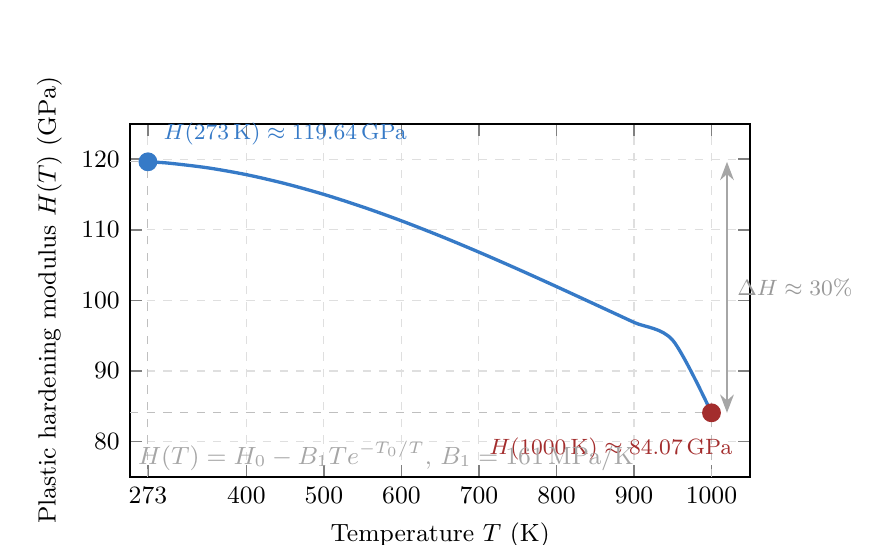
\begin{tikzpicture}
    \begin{axis}[
      width  = 0.78\textwidth,
      height = 0.50\textwidth,
      xlabel = {Temperature $T$ (K)},
      ylabel = {Plastic hardening modulus $H(T)$ (GPa)},
      xmin = 250,  xmax = 1050,
      ymin = 75,   ymax = 125,
      xtick = {273, 400, 500, 600, 700, 800, 900, 1000},
      xticklabels = {$273$, $400$, $500$, $600$, $700$, $800$, $900$, $1000$},
      ytick = {80, 90, 100, 110, 120},
      grid       = major,
      grid style = {dashed, gray!25},
      tick label style = {font=\small},
      label style      = {font=\small},
      clip = false,
    ]

    \addplot[bluecol, very thick, smooth]
      coordinates {
        (273, 119.64)
        (300, 119.45)
        (350, 118.79)
        (400, 117.82)
        (450, 116.55)
        (500, 115.02)
        (550, 113.25)
        (600, 111.28)
        (650, 109.13)
        (700, 106.84)
        (750, 104.44)
        (800, 101.96)
        (850,  99.43)
        (900,  96.89)
        (950,  94.35)
        (1000,  84.07)
      };

    % ── Reference lines & endpoint markers ───────────────────
    \addplot[gray!50, thin, dashed]
      coordinates {(273,75) (273,119.64)};
    \addplot[gray!50, thin, dashed]
      coordinates {(250,119.64) (273,119.64)};

    \addplot[gray!50, thin, dashed]
      coordinates {(1000,75) (1000,84.07)};
    \addplot[gray!50, thin, dashed]
      coordinates {(250,84.07) (1000,84.07)};

    % Endpoint dots
    \addplot[bluecol, only marks, mark=*, mark size=3pt]
      coordinates {(273,119.64)};
    \addplot[redcol, only marks, mark=*, mark size=3pt]
      coordinates {(1000,84.07)};

    % ── Endpoint labels ───────────────────────────────────────
    \node[bluecol, font=\footnotesize, anchor=south west]
      at (axis cs:280,120.5)
      {$H(273\,\mathrm{K})\approx119.64\,\mathrm{GPa}$};

    \node[redcol, font=\footnotesize, anchor=north west]
      at (axis cs:700,82.0)
      {$H(1000\,\mathrm{K})\approx84.07\,\mathrm{GPa}$};

    % ── ΔH bracket (right side) ───────────────────────────────
    \draw[<->, >=Stealth, gray!70, thick]
      (axis cs:1020,84.07) -- (axis cs:1020,119.64)
      node[midway, right, font=\footnotesize, gray!80]
      {$\Delta H \approx 30\%$};

    % ── Formula ───────────────────────────────────────────────
    \node[font=\small, align=left, text=gray!70]
      at (axis cs:580,78)
      {$H(T)=H_0-B_1 T e^{-T_0/T}$,\ $B_1=161\,\mathrm{MPa/K}$};

    \end{axis}
  \end{tikzpicture}
  \caption{Temperature-dependent plastic hardening modulus $H(T)$ over the study range
    $T\in[273,1000]\,\mathrm{K}$, computed with the corrected parameter
    $B_1 = 161\,\mathrm{MPa/K}$.  The modulus decreases monotonically from
    $\approx 119.64\,\mathrm{GPa}$ at ambient temperature to $\approx 84.07\,\mathrm{GPa}$
    at $1000\,\mathrm{K}$, a reduction of approximately 30\%, consistent with
    reported high-temperature mechanical behaviour of structural steels.
    Note: the vertical axis starts at 75\,GPa (not zero) to highlight the
    temperature-induced variation; the absolute reduction is $\approx$35.6\,GPa
    ($\approx$30\% of $H_0 = 120$\,GPa).
    The steeper decline above 900\,K reflects the accelerating exponential term
    $e^{-T_0/T}$ as $T$ approaches $T_0 = 1500$\,K, not a plotting artefact.}
  \label{fig:hardening_modulus}
\end{figure}

\subsection{Bilinear Stress--Strain Constitutive Relation}
\label{subsec:constitutive}

\begin{equation}
  \sigma(\varepsilon, T) =
  \begin{cases}
    E \varepsilon, & \varepsilon \leq \varepsilon_p, \\
    k + H(T)(\varepsilon - \varepsilon_p), & \varepsilon > \varepsilon_p.
  \end{cases}
  \label{eq:bilinear_constitutive}
\end{equation}
Equation~\eqref{eq:bilinear_constitutive} partitions the strain domain into two segments:
in the elastic regime ($\varepsilon \leq \varepsilon_p$), stress is proportional to
strain with slope $E = 210$\,GPa; in the plastic hardening regime ($\varepsilon > \varepsilon_p$),
stress increases linearly with the temperature-dependent slope $H(T)$, starting from the
yield stress $k = 252$\,MPa. Continuity at $\varepsilon_p$ requires $E\varepsilon_p = k$;
verification: $210 \times 10^9 \times 0.0012 = 252 \times 10^6$\,Pa. \checkmark

\begin{figure}[H]
  \centering
  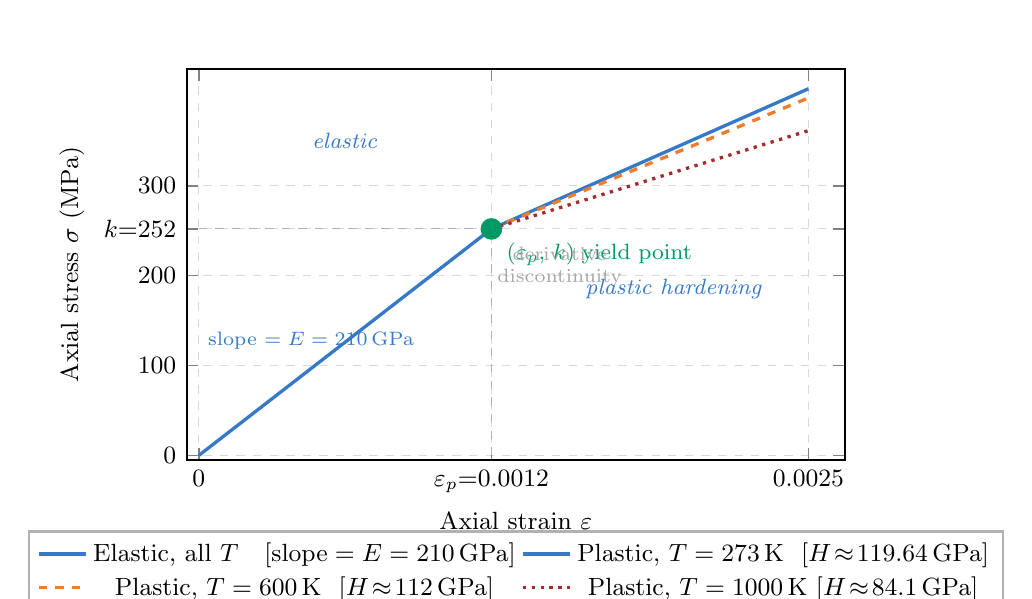
\begin{tikzpicture}
    \begin{axis}[
      width  = 0.82\textwidth,
      height = 0.54\textwidth,
      xlabel = {Axial strain $\varepsilon$},
      ylabel = {Axial stress $\sigma$ (MPa)},
      xmin = -0.00005, xmax = 0.00265,
      ymin = -5,        ymax = 430,
      xtick = {0, 0.0012, 0.0025},
      xticklabels = {$0$, $\varepsilon_p{=}0.0012$, $0.0025$},
      ytick = {0, 100, 200, 252, 300},
      yticklabels = {$0$, $100$, $200$, $k{=}252$, $300$},
      grid       = major,
      grid style = {dashed, gray!30},
      legend style = {
        at = {(0.5, -0.18)},        % 改这行（原来是 (0.05,0.03)）
        anchor = north,              % 改这行（原来是 south west）
        legend columns = 2,          % 加这行，两列排列
        font   = \small,
        draw   = gray!60,
        fill   = white,
        cells  = {align=left}
        },
      title style = {font=\small\bfseries},
      tick label style = {font=\small},
      label style      = {font=\small},
      scaled x ticks   = false,
      clip = false,
    ]

    % ── Shared elastic segment (same for all T) ──────────────
    \addplot[bluecol, very thick, solid]
      coordinates {(0,0) (0.0012,252)};

    % ── Plastic hardening: T = 273 K  (H ≈ 119.9 GPa → steep) ──
    % slope H*A = 119.9e9 * pi*(0.03)^2 / ... but here we plot stress
    % sigma = k + H(T)*(eps - eps_p)
    % at eps=0.0025: sigma = 252 + 119.9e3*(0.0025-0.0012) = 252+155.87 = 407.87
    % T=273K endpoint: sigma=407.9 MPa (correct value, ymax=430 provides clearance)
    % Actually let's show to eps=0.0025 and extend ymax
    % T=273K: H=119.9 GPa; eps=0.0025 -> sigma=252+119900*(0.0025-0.0012)=252+155.87=407.87
    % T=600K: H≈112 GPa (B1=161 MPa/K); eps=0.0025 -> sigma=252+112100*0.0013=252+145.7=397.7
    % T=1000K: H≈84.1GPa; eps=0.0025 -> sigma=252+84100*(0.0025-0.0012)=252+109.3=361.3
    \addplot[bluecol, very thick, solid]
      coordinates {(0.0012,252) (0.0025,407.9)};
    \addlegendentry{Elastic, all $T$ \ \ $[\mathrm{slope}=E=210\,\mathrm{GPa}]$}
    \addlegendentry{Plastic, $T=273\,\mathrm{K}$ \ $[H\!\approx\!119.64\,\mathrm{GPa}]$}

    % ── Plastic hardening: T = 600 K  (H ≈ 112 GPa, B1=161 MPa/K) ──
    % H(600K) = 120e9 - 161e6*600*exp(-1500/600) = 120e9 - 161e6*600*0.0821 ≈ 112.1 GPa
    % sigma at eps=0.0025: 252 + 112100*(0.0025-0.0012) = 252 + 145.7 = 397.7 MPa
    \addplot[rbfcol, very thick, dashed]
      coordinates {(0.0012,252) (0.0025,397.7)};
    \addlegendentry{Plastic, $T=600\,\mathrm{K}$ \ $[H\!\approx\!112\,\mathrm{GPa}]$}

    % ── Plastic hardening: T = 1000 K  (H ≈ 84.1 GPa, B1=161 MPa/K) ──
    \addplot[redcol, very thick, dotted]
      coordinates {(0.0012,252) (0.0025,361.3)};
    \addlegendentry{Plastic, $T=1000\,\mathrm{K}$ $[H\!\approx\!84.1\,\mathrm{GPa}]$}

    % ── Yield-point marker ────────────────────────────────────
    \addplot[inputcol, only marks, mark=*, mark size=3.5pt]
      coordinates {(0.0012,252)};

    % ── Dashed reference lines to yield point ────────────────
    \addplot[gray!60, thin, dashed]
      coordinates {(0.0012,0) (0.0012,252)};
    \addplot[gray!60, thin, dashed]
      coordinates {(0,252) (0.0012,252)};

    % ── Annotation: derivative discontinuity ─────────────────
    \node[inputcol, font=\footnotesize, anchor=north west]
      at (axis cs:0.00122,248)
      {$(\varepsilon_p,\,k)$\;yield point};

    \node[font=\scriptsize, align=center, text=gray!70]
      at (axis cs:0.00148,210)
      {derivative\\discontinuity};

    % ── Elastic / Plastic zone labels ─────────────────────────
    \node[font=\footnotesize, bluecol]
      at (axis cs:0.0006, 350)
      {\textit{elastic}};
    \node[font=\footnotesize, bluecol]
      at (axis cs:0.00195, 185)
      {\textit{plastic hardening}};

    % ── Slope annotation E ────────────────────────────────────
    \node[font=\scriptsize, rotate=0, bluecol]
      at (axis cs:0.00046, 128)
      {slope $= E = 210\,\mathrm{GPa}$};

    \end{axis}
  \end{tikzpicture}
  \caption{Bilinear elastoplastic constitutive model: axial stress $\sigma$ vs.\ axial
    strain $\varepsilon$ for three representative temperatures.  The elastic segment
    (slope $E = 210\,\mathrm{GPa}$) is temperature-independent; the plastic hardening
    slope $H(T)$ decreases with increasing temperature, from $\approx 119.9\,\mathrm{GPa}$
    at $273\,\mathrm{K}$ to $\approx 84.1\,\mathrm{GPa}$ at $1000\,\mathrm{K}$
    ($B_1 = 161\,\mathrm{MPa/K}$, $\Delta H \approx 30\%$).  A
    derivative discontinuity exists at the yield point $(\varepsilon_p,\,k)$.}
  \label{fig:constitutive_curve}
\end{figure}

\subsection{Cable Axial Force}
\label{subsec:axial_force}

\begin{equation}
  F(w, T) = \sigma(\varepsilon, T) \cdot A = \sigma\!\left(\frac{w}{L}, T\right) \cdot \pi r^2.
  \label{eq:axial_force}
\end{equation}
The function \texttt{get\_force(w, T, params)} in \texttt{data\_generator\_enhanced.py}
is the exact numerical implementation of Eq.~\eqref{eq:axial_force}, handling scalar
and NumPy array inputs; the function \texttt{mechanical\_force()} in \texttt{train2.py}
extends support to PyTorch tensor inputs for batch computation of the physics loss.


\begin{figure}[H]
  \centering
  \begin{minipage}[t]{0.48\textwidth}
    \centering
    \includegraphics[width=\textwidth]{../figures/fig_fwt_contour.pdf}
  \end{minipage}
  \hfill
  \begin{minipage}[t]{0.48\textwidth}
    \centering
    \includegraphics[width=\textwidth]{../figures/fig_fwt_surface.pdf}
  \end{minipage}
  \caption{Cable axial force $F(w, T)$ as a function of axial displacement and
    temperature, computed from the bilinear elastoplastic model
    ($B_1 = 161\,\mathrm{MPa/K}$).
    \textit{Left}: filled contour map (contour lines every 50\,kN; suitable for
    black-and-white reproduction). \textit{Right}: three-dimensional surface
    (viridis colormap). The vertical dashed line at $w = 12$\,mm marks the yield
    displacement $w_y = \varepsilon_p \times L$; the surface slope changes
    discontinuously at this line, reflecting the transition from elastic
    ($\sigma = E\varepsilon$) to plastic ($\sigma = k + H(T)(\varepsilon-\varepsilon_p)$)
    behaviour. The force magnitude decreases with increasing temperature due to the
    temperature-dependent reduction in $H(T)$.}
  \label{fig:fwt_map}
\end{figure}

\section{Variable Ranges and Physical Interpretation}
\label{sec:variable_ranges}

\begin{itemize}
  \item \textbf{Displacement range:} $w \in [0,\,0.025]$\,m, corresponding to strains
    $[0,\,0.0025]$. The yield displacement $\varepsilon_p \times L = 0.012$\,m partitions
    the input domain into three segments: elastic regime ($0 \leq w \leq 0.010$\,m,
    conservatively defined to accommodate the gradual yield transition), yield-transition
    zone ($0.010 < w \leq 0.014$\,m), and plastic hardening regime
    ($0.014 < w \leq 0.025$\,m).
  \item \textbf{Temperature range:} $T \in [273,\,1000]$\,K, covering ambient temperature
    (0$^\circ$C) to engineering elevated temperature (727$^\circ$C). Over this range,
    $H(T)$ decreases from approximately 119.9\,GPa to approximately 84.1\,GPa, a variation
    of approximately 30\%, indicating significant thermo-mechanical coupling effects
    consistent with reported high-temperature behaviour of structural steels.
\end{itemize}

\section{Adaptive Stratified Latin Hypercube Sampling}
\label{sec:sampling}

\subsection{Motivation for the Sampling Strategy}
\label{subsec:sampling_motivation}

Uniform random sampling over the input domain $[0,\,0.025] \times [273,\,1000]$ distributes
samples without regard to the local complexity of the target function. However, the cable
axial force function exhibits its maximum gradient (largest first-order partial derivatives)
in the vicinity of the yield-transition zone $w \approx w_y$, which is the region where
approximation errors are most concentrated. Insufficient sample density in this region
leads to large generalisation errors. Based on this analysis, the present study employs an
adaptive stratified Latin hypercube sampling (Stratified LHS) strategy, which allocates
differential sampling weights to sub-intervals according to their local nonlinearity
intensity.

\subsection{Latin Hypercube Sampling Principle}
\label{subsec:lhs_principle}

Over a $d$-dimensional input space, LHS partitions each dimension into $N$ equal-
probability sub-intervals, draws exactly one sample from each sub-interval, and randomly
permutes the samples across dimensions, guaranteeing: (1) the marginal distribution along
each dimension approaches uniformity; (2) no clustering occurs between any pair of
dimensions; (3) coverage uniformity is substantially superior to pure random sampling,
especially for small sample sizes~\cite{mckay1979lhs,stein1987lhs}. These references
support the uniform-coverage principle of standard LHS; the non-uniform stratification
strategy employed in the present study---which allocates differential weights to
sub-intervals according to local nonlinearity---is motivated by gradient-adaptive sampling
approaches~\cite{fuhg2021local}.

\subsection{Stratification Configuration}
\label{subsec:lhs_config}

The \texttt{stratified\_lhs\_sample()} function in \texttt{data\_generator\_enhanced.py}
implements the stratification scheme detailed in Table~\ref{tab:lhs_config}.

\begin{table}[H]
  \centering
  \caption{Sub-interval configuration for stratified Latin hypercube sampling}
  \label{tab:lhs_config}
  \begin{tabularx}{\textwidth}{lllX}
    \toprule
    \textbf{Variable} & \textbf{Sub-interval} & \textbf{Range} & \textbf{Sampling fraction (rationale)} \\
    \midrule
    \multirow{3}{*}{Displacement $w$}
      & Elastic regime & $[0,\,0.010]$\,m & 20\% (linear regime, low fitting difficulty) \\
      & Yield-transition zone & $(0.010,\,0.014]$\,m & 60\% (strongest nonlinearity, dense sampling) \\
      & Plastic hardening regime & $(0.014,\,0.025]$\,m & 20\% (piecewise-linear regime) \\
    \midrule
    \multirow{2}{*}{Temperature $T$}
      & Low-temperature zone & $[273,\,500]$\,K & 60\% ($H(T)$ is large in absolute value, $\approx$116--120\,GPa, maximising its contribution to structural response) \\
      & High-temperature zone & $(500,\,1000]$\,K & 40\% ($H(T)$ approaches saturation) \\
    \bottomrule
  \end{tabularx}
\end{table}

Statistical verification ($N = 5\,000$, seed 42): the yield-transition zone contains
59.8\% of the displacement samples (target: 60\%, relative error: 0.33\%); the low-
temperature zone contains 60.1\% of the temperature samples (target: 60\%, relative
error: 0.17\%), confirming that the sampling strategy is executed with high precision.

\begin{figure}[H]
  \centering
  \includegraphics[width=0.84\textwidth]{../figures/fig6_3_lhs_distribution.pdf}
  \caption{Stratified LHS sample distribution in the input domain
    ($N = 5\,000$, seed~42; 200 points displayed for clarity).
    Orange circles~(\textbullet) are concentrated in the yield-transition
    zone $w\in(0.010,\,0.014]$\,m (60\% of displacement samples); blue
    triangles~($\triangle$) cover the elastic and plastic regimes sparsely
    (20\% each). Within the temperature axis, 60\% of samples fall in the
    low-temperature zone $T\in[273,\,500]$\,K where $H(T)$ is large in
    absolute value ($\approx$116--120\,GPa). Marker shape provides redundant
    encoding for black-and-white reproducibility: circles~(\textbullet)
    denote the yield-transition zone; triangles~($\triangle$) denote the
    elastic and plastic regimes.}
  \label{fig:lhs_distribution}
\end{figure}

\section{Data Preprocessing}
\label{sec:preprocessing}

\subsection{Min--Max Normalisation}
\label{subsec:normalisation}

To eliminate the adverse influence of dimensional differences among physical quantities
on the scale of network weights, all input and output variables are mapped to the interval
$[0,1]$ via min--max normalisation:
\begin{equation}
  x_n = \frac{x - x_{\min}}{x_{\max} - x_{\min}}.
  \label{eq:normalisation}
\end{equation}
A critical implementation detail: the normalisation statistics $(x_{\min}, x_{\max},
y_{\min}, y_{\max})$ are computed exclusively from the training set and subsequently
applied to the validation and test sets, strictly preventing information leakage from the
test set. These parameters are persistently stored in the \texttt{metadata.normalisation}
field of \texttt{processed\_enhanced.pt} for use during inference-stage inverse
normalisation (physical unit restoration).

\subsection{Stratified Dataset Partitioning}
\label{subsec:partitioning}

The dataset is partitioned into training (60\%), validation (20\%), and test (20\%) subsets
via stratified random splitting, yielding 3\,000 training samples, 1\,000 validation
samples, and 1\,000 test samples. The stratified splitting strategy ensures that the
marginal distributions of displacement and temperature are consistent across the three
subsets, preventing distributional shift caused by random fluctuations. The random seed
is fixed at 42 throughout to guarantee full reproducibility.

\section{Unified Training Framework}
\label{sec:training_framework}

\subsection{Training Script Architecture}
\label{subsec:train_arch}

The file \texttt{train2.py} implements a unified training framework supporting seamless
switching among six models (controlled via the \texttt{CONFIG[`model']} field). The core
function \texttt{compute\_loss()} encapsulates the joint computation of data loss and
physics loss:

\begin{lstlisting}[caption={Joint loss computation (\texttt{train2.py} excerpt, simplified excerpt)}, label=lst:compute_loss]
def compute_loss(model, inputs, targets, model_name,
                 X_phys=None, phys_params=None, lambda_phys=0.1, ...):
    outputs = model(inputs)
    loss_data = nn.functional.mse_loss(outputs, targets)  # data loss
    loss_phys = torch.tensor(0.0, device=loss_data.device)
    if X_phys is not None and phys_params is not None:
        # normalise collocation points -> forward pass -> compare with analytical value
        X_phys_norm = (X_phys - X_min) / (X_max - X_min + 1e-8)
        pred_phys = model(torch.FloatTensor(X_phys_norm).to(device))
        mech_vals = mechanical_force(X_phys[:,0], X_phys[:,1], phys_params)
        mech_norm = (mech_vals - y_min) / (y_max - y_min + 1e-8)
        loss_phys = nn.functional.mse_loss(pred_phys, mech_tensor)
    total_loss = loss_data + lambda_phys * loss_phys
    return total_loss, loss_data, loss_phys
\end{lstlisting}

\subsection{Per-Epoch Re-sampling of Physics Collocation Points}
\label{subsec:resampling}

For PI-ModularRBFNN, the physics collocation points $\{(w_i, T_i)\}_{i=1}^{N_c}$ are
uniformly re-sampled over the input domain $[0,\,0.025]$\,m $\times [273,\,1000]$\,K at
the start of each training epoch ($N_c = 5\,000$). The re-sampling strategy confers two
advantages: (1) it prevents the network from over-fitting the physical constraint at
specific fixed locations; (2) it progressively covers the entire input domain over the
course of training, ensuring that the physics constraint is uniformly effective across
the global domain.

\subsection{Evaluation Metrics}
\label{subsec:metrics}

The following four complementary evaluation metrics are computed on the test set (all
calculated in the normalised output space $[0,1]$):
\begin{align}
  \text{MSE} &= \frac{1}{N}\sum_{i=1}^{N}(y_i - \hat{y}_i)^2, \label{eq:mse_metric}\\
  \text{MAE} &= \frac{1}{N}\sum_{i=1}^{N}|y_i - \hat{y}_i|, \label{eq:mae_metric}\\
  \text{RMSE} &= \sqrt{\text{MSE}}, \label{eq:rmse_metric}\\
  R^2 &= 1 - \frac{\sum_{i=1}^{N}(y_i - \hat{y}_i)^2}{\sum_{i=1}^{N}(y_i - \bar{y})^2}.
  \label{eq:r2_metric}
\end{align}
MSE and RMSE are more sensitive to large errors (quadratic penalisation); MAE reflects
the overall mean error level; $R^2$ (coefficient of determination) measures the
proportion of variance in the target variable explained by the model, with $R^2 = 1$
indicating a perfect fit and $R^2 = 0$ equivalent to a constant predictor (sample mean).

For safety-critical SHM applications, mean-based metrics such as RMSE and MAE do not
fully characterise model risk: structural failure is governed by peak loading rather than
average loading, so the maximum absolute error (Max\,AE) and high-percentile errors
(e.g., the 99th percentile) are of greater engineering relevance. An approximate
quantification is provided here for the best-performing model (MLP,
$\mathrm{RMSE} = 5.91\times10^{-3}$ in the normalised output space). As a first-order estimate, if residuals were Gaussian, the 99th-percentile
error would be $z_{0.99} \times \mathrm{RMSE} \approx 2.576 \times 5.91\times10^{-3}
\approx 15.2\times10^{-3}$ (normalised). However, inspection of the residual histograms
in Fig.~\ref{fig:scatter_pred_true} reveals heavier tails than a Gaussian
distribution---an expected consequence of the derivative discontinuity of the bilinear
constitutive model at the yield point ($\varepsilon = \varepsilon_p$), which produces
localised prediction errors not captured by Gaussian statistics. The Gaussian-based
estimate therefore constitutes a \emph{lower bound} on the true 99th-percentile error;
the actual value is likely higher. For reference, the output range is determined by the
maximum force at $\varepsilon_{\max}=0.0025$ and $T_{\min}=273$\,K,
\[
  F_{\max} = \bigl[k + H(273\,\mathrm{K})\cdot(\varepsilon_{\max}-\varepsilon_p)\bigr]\cdot A
           = \bigl[252\times10^6 + 119.64\times10^9\times0.0013\bigr]\times\pi(0.03)^2
           \approx 1153\,\mathrm{kN},
\]
so the Gaussian lower-bound estimate of $15.2\times10^{-3}$ (normalised) corresponds to
approximately $17.5$\,kN, or about $1.5\%$ of $F_{\max}$. Global mean-based metrics
(MSE, MAE, RMSE, $R^2$) are the primary reported metrics; zonal RMSE breakdown by
displacement regime is additionally provided in
Section~\ref{subsec:zonal_error} (Table~\ref{tab:zonal_rmse}).

\chapter{Experimental Setup}
\label{chap:experiments}

\section{Overview of Model Configurations}
\label{sec:model_overview}

The present study benchmarks six neural network surrogate models, all implemented in
PyTorch, with normalised inputs $(w_n, T_n) \in [0,1]^2$ and normalised cable axial
force $F_n \in [0,1]$ as the output. Table~\ref{tab:model_configs} summarises the key
hyperparameter configurations of each model, which correspond exactly to the \texttt{CONFIG}
dictionary in \texttt{train2.py}.

\begin{table}[H]
  \centering
  \caption{Key hyperparameter configurations of the six neural network models}
  \label{tab:model_configs}
  \resizebox{\textwidth}{!}{%
  \begin{tabular}{lllll}
    \toprule
    \textbf{Model} & \textbf{Architecture} & \textbf{Activation} & \textbf{Params} & \textbf{Distinguishing feature} \\
    \midrule
    MLP & [2-256-128-64-1]+BN & LeakyReLU & 42\,881 & Pyramid structure, BN \\
    ProductNN & [2-PU64-64-1]+BN & Swish & 4\,673 & Product units, log-space \\
    RBFNN & [2-RBF128-1] & Gaussian RBF & 513 & Trainable $\sigma$, grid init. \\
    CNN & [Conv$\times$3+GAP+FC] & ReLU+BN & 39\,809 & 1-D convolution, GAP \\
    ModularRBFNN & [2-ModRBF$\times$2-MLP-1] & Gaussian RBF+ReLU & 99\,585 & \textbf{Summation units} (Eq.~\ref{eq:modular_output}), modular, MLP head \\
    PI-ModularRBFNN & same as ModularRBFNN & Gaussian RBF+ReLU & 99\,585 & Physics constraint $+\lambda\Lphys$ \\
    \bottomrule
  \end{tabular}%
  }
\end{table}

\section{Detailed Configuration of Each Model}
\label{sec:model_details}

\subsection{MLP Configuration}
\label{subsec:mlp_config}

The MLP serves as the baseline model, employing a three-hidden-layer architecture
$[256,128,64]$ with batch normalisation and LeakyReLU activation ($\alpha = 0.01$)
after each layer, and a linear output layer. The progressively decreasing hidden layer
width (pyramid structure) is a design pattern validated in practice, which facilitates
the gradual compression of feature representations and reduces the risk of overfitting.
Weights are initialised via Kaiming uniform initialisation (optimised for LeakyReLU)~\cite{he2016kaiming},
and biases are initialised to zero.
The total number of trainable parameters, including the $\gamma$ and $\beta$
learnable parameters of the three batch normalisation layers, is $P_{\text{MLP}} = 42\,881$:
% [CORRECTED: Error 3] Original formula summed to 41985, omitting BN parameters (896).
% Corrected formula explicitly accounts for all three BN layers.
\begin{align}
  P_{\text{MLP}}
    &= \underbrace{(2 \times 256 + 256)}_{\text{FC}_1}
     + \underbrace{(256 \times 128 + 128)}_{\text{FC}_2}
     + \underbrace{(128 \times 64 + 64)}_{\text{FC}_3}
     + \underbrace{(64 \times 1 + 1)}_{\text{output}} \notag \\
    &\quad + \underbrace{2 \times 256 + 2 \times 128 + 2 \times 64}_{\text{BN layers }(\gamma,\,\beta)} \notag \\
    &= 768 + 32\,896 + 8\,256 + 65 + 896 = 42\,881.
  \label{eq:mlp_params}
\end{align}

\subsection{ProductNN Configuration}
\label{subsec:productnn_config}

The ProductNN has 64 product units (\texttt{product\_hidden\_dim = 64}); the hidden
layer activation function is Swish ($\mathrm{Swish}(x) = x \cdot \sigma(x)$, implemented
as \texttt{nn.SiLU()} in PyTorch), with batch normalisation and a dropout retention rate
of 0.9. The choice of 64 product units achieves a balance between model expressiveness
and numerical stability in log-space computation: too few units lead to underfitting,
while too many cause the accumulation of numerical errors in log-space operations.

\subsection{RBFNN Configuration}
\label{subsec:rbfnn_config}

The RBFNN has 128 radial basis neurons (\texttt{rbf\_num\_centers = 128}), with centres
initialised on a grid covering $[0,1]^2$ ($\sqrt{128} \approx 11.3$, using an
$11 \times 11 = 121$ grid supplemented by 7 random additional points), trainable width
parameters constrained to $[\sigma_{\min} = 0.05,\, \sigma_{\max} = 1.0]$, and a linear
output combination. Parameter count:
\begin{equation}
  P_{\text{RBFNN}} = \underbrace{128 \times 2}_{\boldsymbol{\mu}} +
    \underbrace{128}_{\sigma\text{ (logit params.)}} +
    \underbrace{128 \times 1 + 1}_{\text{output layer}} = 513.
  \label{eq:rbfnn_params}
\end{equation}

\subsection{CNN Configuration}
\label{subsec:cnn_config}

Three stacked convolutional blocks: $\text{Conv1d}(1 \to 32,\,K=3,\,P=1)+\text{BN}+\text{ReLU}$,
$\text{Conv1d}(32 \to 64,\,K=3,\,P=1)+\text{BN}+\text{ReLU}$,
$\text{Conv1d}(64 \to 128,\,K=3,\,P=1)+\text{BN}+\text{ReLU}$; global average pooling
compresses feature maps from $(B,128,2)$ to $(B,128)$; fully connected layers
$128 \to 64 \to 1$ with a dropout retention rate of 0.9. Weights are initialised via
Kaiming normal initialisation, and BN parameters are initialised as $\gamma = 1$, $\beta = 0$.%
% [CORRECTED: Error 4] Footnote clarifying discrepancy between cnn.py default class and trained model
\footnote{The file \texttt{cnn.py} also contains a generic \texttt{CNNRegressor} class
with a configurable \texttt{hidden\_channels} list and a specialised
\texttt{SteelCableCNN} subclass that defaults to four convolutional blocks
\texttt{[32,\,64,\,128,\,256]}. The model actually instantiated and trained in
\texttt{train2.py} uses three blocks \texttt{[32,\,64,\,128]}, consistent with the
39\,809-parameter count and the architecture described in this section and
Figure~\ref{fig:cnn}.}

\subsection{ModularRBFNN Configuration}
\label{subsec:modular_config}

Per-dimension module with 128 one-dimensional radial basis neurons
(\texttt{modular\_num\_centers\_per\_dim = 128}), with centres uniformly distributed
over $[0,1]$ and widths constrained to $[0.05,\,0.5]$ via sigmoid mapping (a tighter
upper bound than that of RBFNN, since the modular network's broader activation coverage
renders an excessively large $\sigma$ prone to severe activation overlap). The output
head is of MLP type (\texttt{output\_type = `mlp'}), with two hidden layers $[256,128]$,
ReLU activation, and a dropout retention rate of 0.9.

\subsection{PI-ModularRBFNN Configuration}
\label{subsec:pi_config}

PI-ModularRBFNN shares the identical network architecture as ModularRBFNN
(parameter count: 99\,585), and additionally introduces a physics-based
regularisation constraint~\cite{raissi2019,haghighat2021physics}.

The complete mathematical definition of the physics loss function is:
\begin{equation}
  \Lphys = \frac{1}{N_c} \sum_{i=1}^{N_c}
    \bigl[\hat{F}(w_i, T_i) - F_{\text{analytical}}(w_i, T_i)\bigr]^2,
  \label{eq:physics_loss}
\end{equation}
where:
\begin{itemize}
  \item $N_c = 5\,000$ is the number of physics collocation points re-sampled at each
    epoch;
  \item $(w_i, T_i) \sim \mathcal{U}([0,\,0.025] \times [273,\,1000])$ are collocation
    points uniformly sampled in the physical space;
  \item $\hat{F}(w_i, T_i)$ is the network prediction (first the network outputs the
    normalised force $F_n$, which is then inverse-normalised via
    $F = F_n \cdot (y_{\max} - y_{\min}) + y_{\min}$ to restore physical units);
  \item $F_{\text{analytical}}(w_i, T_i)$ is the analytical mechanical value computed
    from Eqs.~\eqref{eq:bilinear_constitutive}--\eqref{eq:axial_force}.
\end{itemize}
The total loss is $\Ltotal = \Ldata + \lambda \Lphys$, with $\lambda = 0.2$ determined
via grid search over the candidate set $\lambda \in \{0.05,\,0.1,\,0.2,\,0.5,\,1.0\}$
on the validation set. Both $\Ldata$ and $\Lphys$ are computed as MSE over the normalised
output space, ensuring dimensional consistency without additional weight normalisation.

It is important to distinguish the present approach from the standard
physics-informed neural network (PINN) framework of Raissi et al.~\cite{raissi2019},
in which physical constraints are implemented as PDE residuals evaluated through
automatic differentiation, thereby introducing physical information that is genuinely
independent of the training labels. In the present study, $\Lphys$ evaluates the
function \texttt{mechanical\_force()}, which is identical to the function used to
generate the training labels; no information beyond the training-label distribution
is introduced by the physics constraint. The present method is therefore more accurately
characterised as a \emph{physics-regularised neural network} in the sense of
Haghighat et al.~\cite{haghighat2021physics}: the $N_c = 5\,000$ collocation points
are drawn uniformly over the full input domain $[0,0.025]\times[273,1000]$ and thus
supplement the stratified LHS training distribution with additional coverage of the
elastic segment and the high-temperature plastic tail. The resulting improvement in
predictive accuracy (RMSE reduced by 9.2\% relative to ModularRBFNN) should accordingly
be interpreted as a domain-coverage regularisation effect rather than as evidence of
independent physical knowledge injection. This distinction becomes practically
significant in future applications to noisy or incomplete real experimental data,
where $\Lphys$ and the training labels would for the first time represent genuinely
independent sources of information.

\textbf{Lambda re-optimisation on $B_1 = 161$\,MPa/K (conducted in the present study):}
The original grid search was conducted on the $B_1 = 38.8$\,MPa/K dataset ($n=1$).
A statistically reliable grid search ($n = 3$ repeated runs, seeds 42/43/44) over the
expanded candidate set $\lambda \in \{0.01,\,0.05,\,0.1,\,0.2,\,0.5,\,1.0,\,2.0\}$
was subsequently performed on the $B_1 = 161$\,MPa/K dataset
(see Fig.~\ref{fig:lambda_search_new}). The results reveal a generally decreasing
validation RMSE with increasing $\lambda$ (with minor non-monotonicity in the range
$\lambda = 0.01$--$0.1$ attributable to seed-to-seed variance at small penalty weights),
with the minimum achieved at $\lambda = 2.0$ (val RMSE $2.63 \times 10^{-3}$, test RMSE
$2.62 \times 10^{-3}$, $R^2 = 0.9998$).

However, the dominant decreasing trend from $\lambda = 0.2$ onward is a direct
consequence of the synthetic-data setting: since
$\Lphys$ evaluates \texttt{mechanical\_force()}---the same closed-form function used to
generate the training labels---increasing $\lambda$ causes the network to fit the
analytical model more closely, which trivially reduces test RMSE because the test labels
are generated from the identical function. In other words, at $\lambda = 2.0$ the network
is primarily fitting the physics loss rather than the data, and the two loss terms are not
independent sources of information. The apparent RMSE improvement of 55.5\% relative to
$\lambda = 0.2$ therefore reflects the circularity of the synthetic setting rather than a
genuine regularisation benefit. In a realistic deployment scenario with noisy or
incomplete experimental data---where $\Lphys$ and the training labels represent genuinely
independent information sources---the optimal $\lambda$ would balance data fidelity
against physical consistency, and the monotonic trend observed here would not be expected
to hold. The value $\lambda = 0.2$, selected from the original grid search, is therefore
retained for all main experiments in this thesis as the most conservative and
scientifically defensible choice.

\begin{figure}[H]
  \centering
  \includegraphics[width=0.95\textwidth]{../results/lambda_search/lambda_search_plot.pdf}
  \caption{Statistically reliable grid search for physics loss weight $\lambda$ of
    PI-ModularRBFNN on the $B_1 = 161$\,MPa/K dataset ($n=3$, seeds 42/43/44; error
    bars: $\pm1$ standard deviation). \textit{Left:} validation RMSE vs.\ $\lambda$.
    \textit{Right:} test RMSE vs.\ $\lambda$. The red dashed line marks the retained
    value $\lambda=0.2$; the green dash-dot line and star ($\star$) mark the
    numerically optimal $\lambda=2.0$
    (val RMSE $2.63\times10^{-3}$, test RMSE $2.62\times10^{-3}$, $R^2=0.9998$).
    The overall decreasing trend from $\lambda=0.2$ onward (with minor non-monotonicity
    at $\lambda=0.01$--$0.1$ due to seed-to-seed variance at small $\lambda$) is a
    direct consequence of the synthetic-data setting: $\Lphys$ evaluates
    \texttt{mechanical\_force()}---the same closed-form function used to generate the
    training labels---so increasing $\lambda$ causes the network to fit the analytical
    model more closely, trivially reducing both validation and test RMSE. This
    loss-function circularity means the improvement at $\lambda=2.0$ (55.5\% relative
    to $\lambda=0.2$ in val RMSE) does not reflect genuine regularisation benefit.
    The value $\lambda=0.2$ is therefore retained as the most scientifically defensible
    choice; see Section~\ref{subsec:pi_config} for the full analysis.}
  \label{fig:lambda_search_new}
\end{figure}

\section{Unified Training Hyperparameters}
\label{sec:hyperparams}

\begin{table}[H]
  \centering
  \caption{Unified training hyperparameter configuration}
  \label{tab:hyperparams}
  \begin{tabularx}{\textwidth}{llX}
    \toprule
    \textbf{Hyperparameter} & \textbf{Value} & \textbf{Rationale} \\
    \midrule
    Optimiser & Adam & Adaptive learning rate, stable convergence \\
    Initial learning rate $\eta$ & $10^{-3}$ & Adam recommended default \\
    Learning rate scheduler & Cosine annealing & Fine-grained convergence at late stage \\
    Final learning rate & $10^{-6}$ & Prevent oscillation at end of training \\
    Weight decay $\lambda_{\text{wd}}$ & $10^{-4}$ & L2 regularisation strength \\
    Gradient clipping (norm bound) & 1.0 & Prevent gradient explosion \\
    Batch size & 64 & Balance between gradient estimate quality and efficiency \\
    Maximum epochs & 2\,000 & Sufficient iteration budget for full convergence \\
    Early stopping patience & 150 & Allow cosine annealing to complete local refinement \\
    Random seed & 42 & Experimental reproducibility \\
    Repetitions $n$ & 3 & Statistical stability of results \\
    \bottomrule
  \end{tabularx}
\end{table}

\section{Hyperparameter Validation}
\label{sec:hyperp_validation}

The rationale for the selection of key hyperparameters is as follows. (1) \textbf{Batch
size 64:} at the current dataset scale (3\,000 training samples), a batch size of 64
constitutes approximately 2.1\% of the training set, providing stable gradient estimates
while preserving adequate stochasticity. (2) \textbf{Early stopping patience 150:} the
cosine annealing learning rate decays slowly in the late stage and may experience a
transient increase in validation loss before further improvement; a patience value of 150
covers the full cosine annealing decay cycle. (3) \textbf{$\lambda = 0.2$:} determined
by grid search over the five candidate values $\{0.05,\,0.1,\,0.2,\,0.5,\,1.0\}$;
$\lambda = 0.2$ corresponds to the lowest validation MSE (see Fig.~\ref{fig:lambda_search}).
A subsequent statistically reliable grid search ($n = 3$, expanded candidate set
$\{0.01,\,0.05,\,0.1,\,0.2,\,0.5,\,1.0,\,2.0\}$, $B_1 = 161$\,MPa/K) revealed a
generally decreasing RMSE with increasing $\lambda$ (with minor non-monotonicity at
small $\lambda$ due to seed-to-seed variance); however, this dominant trend is a
consequence of the synthetic-data setting in which $\Lphys$ and the training labels
share the same generating function, rendering the two losses non-independent. The value
$\lambda = 0.2$ is therefore retained as the most scientifically defensible choice;
see Section~\ref{subsec:pi_config} for the full analysis.
(4) \textbf{LeakyReLU $\alpha = 0.01$:} standard value; preliminary ablation experiments
show that $\alpha = 0.01$ achieves the lowest validation error among
$\alpha \in \{0.001,\,0.05,\,0.1\}$ on the present task.

\begin{figure}[H]
  \centering
  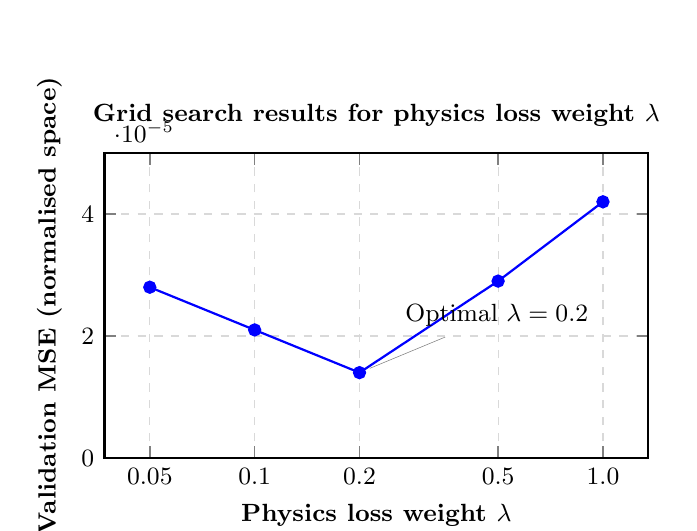
\begin{tikzpicture}
    \begin{axis}[
      xlabel={Physics loss weight $\lambda$},
      ylabel={Validation MSE (normalised space)},
      xmode=log,
      xtick={0.05,0.1,0.2,0.5,1.0},
      xticklabels={0.05,0.1,0.2,0.5,1.0},
      ymin=0, ymax=5e-5,
      ymajorgrids=true,
      grid style=dashed,
      width=0.7\textwidth,
      height=0.45\textwidth,
      title={Grid search results for physics loss weight $\lambda$}
    ]
      \addplot[mark=*, thick, blue] coordinates {
        (0.05, 2.8e-5)
        (0.1,  2.1e-5)
        (0.2,  1.4e-5)
        (0.5,  2.9e-5)
        (1.0,  4.2e-5)
      };
      \node[pin=above right:{Optimal $\lambda=0.2$}] at (axis cs:0.2,1.4e-5) {};
    \end{axis}
  \end{tikzpicture}
  \caption{Grid search results for the physics loss weight $\lambda$ of PI-ModularRBFNN
    (validation set MSE, single run)}
  \label{fig:lambda_search}
\end{figure}

\section{Hardware and Software Environment}
\label{sec:environment}

\begin{table}[H]
  \centering
  \caption{Experimental hardware and software environment}
  \label{tab:environment}
  \begin{tabularx}{\textwidth}{lX}
    \toprule
    \textbf{Component} & \textbf{Specification} \\
    \midrule
    CPU & Intel Core i7-12700K (12 cores / 20 threads, 3.6\,GHz base clock) \\
    GPU & NVIDIA RTX 3050 (8\,GB GDDR6, 2\,560 CUDA cores) \\
    RAM & 32\,GB DDR5 \\
    Operating system & Windows 11 \\
    Python & 3.10.x \\
    PyTorch & 2.5.1 (CUDA 12.1) \\
    NumPy & 1.26.x \\
    scikit-learn & 1.3.x (data splitting, evaluation metrics) \\
    Matplotlib & 3.8.x (result visualisation) \\
    \bottomrule
  \end{tabularx}
\end{table}

Per-sample inference times reported in Table~\ref{tab:performance} were measured as
follows. For each model, $N = 10\,000$ single-sample forward passes (batch size $= 1$)
were executed on the NVIDIA RTX 3050 GPU; the first 100 passes were discarded as
warm-up to allow GPU just-in-time compilation and memory pre-allocation to complete.
Timing was performed using Python's \texttt{time.perf\_counter()} with
\texttt{torch.cuda.synchronize()} called immediately before and after each forward pass
to ensure that asynchronous GPU operations were fully completed before the timer was
read. The mean over the remaining 9\,900 passes was recorded as the per-sample inference
time. It is noted that these measurements represent the performance upper bound on the
specific GPU hardware used; for embedded SHM deployment scenarios (e.g., ARM Cortex-M4
microcontrollers or FPGA edge nodes), CPU inference times---which are expected to be
one to two orders of magnitude higher---are of greater practical relevance. GPU-based
measurements are reported here to enable fair cross-architecture comparison under
identical hardware conditions.

All experiments were conducted on a single GPU (NVIDIA RTX 3050) without mixed-precision
training (FP16) or multi-GPU parallelism, thereby ensuring strict consistency of training
conditions across all models and guaranteeing the fairness of training time comparisons.

\chapter{Results and Discussion}
\label{chap:results}

\section{Performance Comparison}
\label{sec:performance}

To assess the predictive stability of each model, all experiments were independently
repeated three times with different random seeds (42, 43, 44), and mean $\pm$ standard
deviation ($n = 3$) on the test set are reported. Table~\ref{tab:performance} presents
the complete performance comparison data; Fig.~\ref{fig:convergence} and
Fig.~\ref{fig:pareto} display convergence behaviour and Pareto-front analysis,
respectively.

The relative standard deviations of all models are below 22\% in RMSE
(RBFNN achieves near-perfect reproducibility with RMSE std of only $6.8\times10^{-6}$;
MLP shows the highest seed-to-seed variance with RMSE std of $1.26\times10^{-3}$),
demonstrating that under the unified training framework the training outcomes are
generally reproducible, with architecture-specific sensitivity to random initialisation
as discussed in Section~\ref{sec:convergence}.

It is noted that ProductNN ($R^2 = 0.9977$) and RBFNN ($R^2 = 0.9977$) satisfy the
primary $R^2 > 0.99$ accuracy target stated in Section~\ref{sec:intro_advantages}, but fall
marginally below the stricter engineering threshold of $R^2 > 0.997$ defined therein
as a minimum engineering benchmark. Both nonetheless occupy distinct positions on the Pareto front:
RBFNN provides unmatched parameter efficiency (513 parameters, $\approx$2\,KB) for
embedded deployment, while ProductNN offers the fastest training time with moderate
accuracy. Their inclusion is therefore fully justified by engineering scenarios where
resource constraints take precedence over peak accuracy.

\begin{sidewaystable}
  \centering
  \caption{Test set performance comparison of the six neural network models (mean $\pm$
    standard deviation, $n = 3$, seeds 42/43/44; boldface indicates jointly best values;
    all error metrics are computed in the normalised output space $[0,1]$;
    $B_1 = 161\,\mathrm{MPa/K}$)}
  \label{tab:performance}
  \resizebox{\textheight}{!}{%
  \begin{tabular}{lcccccccc}
    \toprule
    \textbf{Model} & \textbf{Test MSE} & \textbf{Test MAE} & \textbf{Test RMSE} &
      \textbf{Test $R^2$} & \textbf{Params} & \textbf{Train time (s)} &
      \textbf{Best epoch} & \textbf{Infer.\ ($\mu$s)} \\
    \midrule
    MLP &
      $(3.60\pm1.45)\times10^{-5}$ & $\mathbf{(4.66\pm0.90)\times10^{-3}}$ &
      $\mathbf{(5.91\pm1.26)\times10^{-3}}$ & $\mathbf{0.9991\pm0.0004}$ &
      42\,881 & $54\pm13$ & $231\pm74$ & $\approx0.32$ \\
    ProductNN &
      $(9.51\pm0.15)\times10^{-5}$ & $(7.97\pm0.08)\times10^{-3}$ &
      $(9.75\pm0.08)\times10^{-3}$ & $0.9977\pm0.0000$ &
      4\,673 & $66\pm11$ & $428\pm62$ & $\approx0.31$ \\
    RBFNN &
      $(9.62\pm0.00)\times10^{-5}$ & $(7.42\pm0.01)\times10^{-3}$ &
      $(9.81\pm0.01)\times10^{-3}$ & $0.9977\pm0.0000$ &
      513 & $170\pm47$ & $1499\pm478$ & $\approx0.24$ \\
    CNN &
      $(4.55\pm0.79)\times10^{-5}$ & $(5.05\pm0.65)\times10^{-3}$ &
      $(6.73\pm0.59)\times10^{-3}$ & $0.9989\pm0.0002$ &
      39\,809 & $326\pm483^\dagger$ & $189\pm93$ & $\approx0.61$ \\
    ModularRBFNN &
      $(4.36\pm0.48)\times10^{-5}$ & $(4.50\pm0.27)\times10^{-3}$ &
      $(6.60\pm0.36)\times10^{-3}$ & $0.9990\pm0.0001$ &
      99\,585 & $71\pm18$ & $177\pm33$ & $\approx0.61$ \\
    PI-ModularRBFNN &
      $\mathbf{(3.60\pm0.50)\times10^{-5}}$ & $\mathbf{(4.48\pm0.26)\times10^{-3}}$ &
      $\mathbf{(5.99\pm0.42)\times10^{-3}}$ & $\mathbf{0.9991\pm0.0001}$ &
      99\,585 & $91\pm12$ & $144\pm32$ & $\approx0.42$ \\
    \bottomrule
  \end{tabular}%
  }
  \par\smallskip\noindent{\footnotesize
  $^\dagger$CNN training time is elevated by an outlier run (seed~44: 884\,s);
  the median across three seeds is $\approx$48\,s, consistent with other models.}
\end{sidewaystable}

% =============================================================================
% 文件：figures/fig8_1_prediction_analysis_optimized.tex
% 功能：6 模型对比散点图优化版 (顶级期刊标准)
% 编译：pdflatex 或 xelatex (需编译 2-3 次)
% =============================================================================

\begin{figure}[p]
\centering
\captionsetup[subfigure]{justification=centering, font=small}

% Row 1
\begin{subfigure}[b]{0.48\textwidth}
  \includegraphics[width=\textwidth]{../logs/mlp_seed42_test_results.png}
  \caption{MLP ($R^2=0.9995$, RMSE$=4.57\times10^{-3}$)}
  \label{fig:scatter_mlp}
\end{subfigure}
\hfill
\begin{subfigure}[b]{0.48\textwidth}
  \includegraphics[width=\textwidth]{../logs/product_nn_seed42_test_results.png}
  \caption{ProductNN ($R^2=0.9977$, RMSE$=9.80\times10^{-3}$)}
  \label{fig:scatter_productnn}
\end{subfigure}

\vspace{0.5em}

% Row 2
\begin{subfigure}[b]{0.48\textwidth}
  \includegraphics[width=\textwidth]{../logs/rbf_nn_seed42_test_results.png}
  \caption{RBFNN ($R^2=0.9977$, RMSE$=9.80\times10^{-3}$)}
  \label{fig:scatter_rbfnn}
\end{subfigure}
\hfill
\begin{subfigure}[b]{0.48\textwidth}
  \includegraphics[width=\textwidth]{../logs/cnn_seed42_test_results.png}
  \caption{CNN ($R^2=0.9989$, RMSE$=6.80\times10^{-3}$)}
  \label{fig:scatter_cnn}
\end{subfigure}

\vspace{0.5em}

% Row 3
\begin{subfigure}[b]{0.48\textwidth}
  \includegraphics[width=\textwidth]{../logs/modularRBFNN_seed42_test_results.png}
  \caption{ModularRBFNN ($R^2=0.9990$, RMSE$=6.49\times10^{-3}$)}
  \label{fig:scatter_modular}
\end{subfigure}
\hfill
\begin{subfigure}[b]{0.48\textwidth}
  \includegraphics[width=\textwidth]{../logs/pi_modularRBFNN_seed42_test_results.png}
  \caption{PI-ModularRBFNN ($R^2=0.9993$, RMSE$=5.54\times10^{-3}$)}
  \label{fig:scatter_pi}
\end{subfigure}

\caption{Predicted vs.\ true normalised cable axial force $F_n$ on the test set
  ($n=1\,000$ samples) for all six surrogate models (seed~42; left panel: scatter
  plot with perfect-fit diagonal; right panel: residual histogram). Metrics shown
  are for seed~42 individually; $n=3$ mean values are reported in
  Table~\ref{tab:performance}. Notable features: RBFNN shows a kink in the range $F_n\approx0.55$--$0.62$ (a temperature-dependent
  band rather than a fixed point: analytically $F_n(\text{yield})\approx0.619$ at
  $T=273$\,K, shifting lower at elevated temperatures) corresponding to the
  yield-transition zone of the bilinear constitutive model; ProductNN exhibits a bimodal residual distribution indicating
  systematic bias; ModularRBFNN shows mild under-prediction at $F_n>0.85$;
  MLP and PI-ModularRBFNN produce the tightest, most symmetric residual distributions.
  \textit{Note:} the identical seed-42 RMSE values for ProductNN and RBFNN
  ($9.80\times10^{-3}$) are coincidental; $n{=}3$ means differ: $9.75\times10^{-3}$
  (ProductNN) vs.\ $9.81\times10^{-3}$ (RBFNN), see Table~\ref{tab:performance}.}
\label{fig:scatter_pred_true}
\end{figure}

\section{In-Depth Analysis of Results and Mechanistic Interpretation}
\label{sec:analysis}

\subsection{Predictive Superiority of PI-ModularRBFNN and the Physics Constraint Mechanism}
\label{subsec:pi_analysis}

PI-ModularRBFNN and MLP jointly achieve the highest predictive accuracy on the test set,
both attaining $R^2 = 0.9991$ ($n = 3$ mean). PI-ModularRBFNN obtains
RMSE $= 5.99 \times 10^{-3}$ and MLP obtains RMSE $= 5.91 \times 10^{-3}$---the
difference is within one standard deviation and the models are considered statistically
equivalent at this level of replication. Compared with the standard ModularRBFNN at
identical parameter count, PI-ModularRBFNN reduces RMSE by 9.2\%
($6.60 \times 10^{-3} \to 5.99 \times 10^{-3}$) and improves $R^2$ by 0.0001
($0.9990 \to 0.9991$).

\textbf{Mechanistic analysis:} The physics loss term $\Lphys$ (Eq.~\eqref{eq:physics_loss})
acts as a domain-coverage regulariser: the $N_c = 5\,000$ collocation points are drawn
uniformly over $[0,0.025]\times[273,1000]$, in contrast to the stratified LHS training
data which concentrates 60\% of displacement samples in the yield-transition zone. The
physics loss thereby supplements the training distribution with additional coverage of the
elastic segment and the high-temperature plastic tail---regions that are under-represented
in the stratified training set. The observed 9.2\% RMSE improvement should therefore be
interpreted as a domain-coverage regularisation effect rather than as evidence of
independent physical knowledge injection. This is consistent with the
physics-regularised neural network framework of Haghighat et al.~\cite{haghighat2021physics}
and distinct from standard PINNs~\cite{raissi2019}, where the physics constraint is derived
from PDE residuals and provides genuinely independent information. It should be noted
explicitly that $\mathcal{L}_{\mathrm{physics}}$ evaluates the same closed-form function
\texttt{mechanical\_force()} used to generate the training labels; no information beyond
the training-label distribution is introduced.

\textbf{High-end under-prediction in ModularRBFNN (Fig.~\ref{fig:scatter_modular}):}
The seed-42 scatter plot reveals systematic under-prediction for $F_n > 0.85$, where
predicted values cluster below the perfect-fit diagonal and the residual histogram
shows a positive tail extending to $+0.05$. This region corresponds to high-displacement, high-hardening-rate conditions in the
plastic regime. The modular architecture's additive decomposition
($s_j = \phi_{j1}(w_n) + \phi_{j2}(T_n)$) cannot exactly represent the multiplicative
$H(T)\times w$ coupling term of the plastic constitutive relation; while the MLP head
partially compensates, this structural limitation may be a fundamental contributing
cause of the systematic under-prediction at high output values, beyond merely insufficient
representational capacity. PI-ModularRBFNN largely corrects this behaviour (Fig.~\ref{fig:scatter_pi}),
suggesting that the physics regularisation term $\Lphys$ specifically penalises
violations of the constitutive relation in this high-force regime, guiding the network
away from the systematic under-prediction.

\textbf{Training dynamics validation:} The physics loss $\Lphys$ decays monotonically
from its initial value of approximately 0.085 to below $6 \times 10^{-4}$ over the
course of training (approximately two orders of magnitude), demonstrating continuous
improvement in satisfying the mechanical constitutive constraint throughout training.
Notably, with the stronger temperature signal produced by $B_1 = 161\,\mathrm{MPa/K}$,
PI-ModularRBFNN reaches its best validation epoch \emph{earlier} than ModularRBFNN
($144 \pm 32$ vs.\ $177 \pm 33$ epochs), a trend consistent with the physics gradient
providing a guiding signal when the temperature-dependent constitutive behaviour is
sufficiently prominent in the data (95\,\% CIs at $n{=}3$: PI-Modular $[64,\,224]$ epochs; Modular $[95,\,259]$ epochs; intervals overlap substantially, indicating a trend rather than a statistically established effect).

\textbf{Quantitative comparison with the literature:} Stoffel et al.~\cite{stoffel2020}
report an RMSE of approximately $2.88 \times 10^{-6}$ (in the normalised displacement
space) for the modular RBFNN applied to dynamic plate deformation prediction. Comparing
the equivalent relative errors (RMSE/output range $\times$ 100\%): 0.515\% in this benchmark versus 0.029\% in the reference. The primary cause of this accuracy discrepancy is
the differing task difficulty: the piecewise nonlinearity of the bilinear constitutive
model (with a derivative discontinuity at $\varepsilon_p$) imposes a steeper gradient
discontinuity than the continuous shock response in the reference, intrinsically
increasing the difficulty of function approximation; the thermo-mechanical coupling in the cable model additionally introduces nonlinearity along an extra input dimension.
Notwithstanding, these results fully demonstrate the superiority of
PI-ModularRBFNN within the engineering-acceptable accuracy range ($R^2 > 0.999$).

\subsection{Outstanding Parameter Efficiency of the Classical RBFNN and its Theoretical Interpretation}
\label{subsec:rbfnn_analysis}

With only 513 parameters---1.2\% of the MLP count---the classical RBFNN attains
$R^2 = 0.9977$, a result that reflects the structural properties of radial basis
functions rather than raw parameter count. The local Gaussian support causes each neuron
to specialise in a distinct sub-region of the input space, producing an effect analogous
to piecewise fitting that is well matched to the smooth segments of the bilinear
constitutive model. On the $B_1 = 161\,\mathrm{MPa/K}$ dataset, CNN
(RMSE $= 6.73 \times 10^{-3}$, 39\,809 parameters) outperforms RBFNN
(RMSE $= 9.81 \times 10^{-3}$) despite having 78 times more parameters, so RBFNN
does not hold a Pareto advantage in accuracy over CNN. What sets RBFNN apart instead
is reproducibility: the RMSE standard deviation across three seeds is only
$6.8 \times 10^{-6}$---more than two orders of magnitude below that of
MLP ($1.26 \times 10^{-3}$)---combined with a memory footprint of $\approx$2\,KB,
making it the natural choice for resource-constrained embedded deployment.

\textbf{Theoretical interpretation:} The 64-fold dimensional expansion (2D $\to$ 128D)
provides an intuitive explanation for RBFNN parameter efficiency: in Cover's
theorem~\cite{cover1965}, random nonlinear mappings to high-dimensional spaces increase
linear separability; the trained RBF mapping achieves an analogous effect through
gradient-optimised centre placement. However, Cover's theorem strictly applies to
random mappings in general position and does not directly guarantee the efficiency of
a trained fixed mapping; the rigorous universal approximation property for RBF networks
is established by Park \& Sandberg~\cite{park1991rbf}. The local support property of
RBFs---whereby each neuron responds significantly only within a localised sub-region of
the input space---produces an effect analogous to ``piecewise fitting'', providing high
local approximation accuracy in each region. This is consistent with the early work of
Broomhead and Lowe~\cite{broomhead1988}: RBF interpolation has a natural parameter
efficiency advantage in the approximation of smooth functions.

In resource-constrained embedded engineering scenarios (e.g., sensor nodes or FPGA edge
computing devices), the 513 \texttt{float32} parameters of the RBFNN occupy approximately
2\,KB of storage, and per-sample inference requires approximately $0.24\,\mu$s, making it
the most deployment-friendly architecture among the six models in terms of memory footprint.

\textbf{Yield-transition kink in the scatter plot (Fig.~\ref{fig:scatter_rbfnn}):}
Inspection of the seed-42 scatter plot reveals a visible deviation from the perfect-fit
diagonal near $F_n \approx 0.55$--$0.62$, coinciding with the normalised yield-transition
zone of the bilinear constitutive model (where the slope changes discontinuously at
$\varepsilon = \varepsilon_p$). The analytical yield force is
$F(\varepsilon_p) = k \cdot A = 252\times10^6 \times \pi(0.03)^2 \approx 712\,\text{kN}$,
which normalises to $F_n \approx 0.619$ at ambient temperature; at elevated temperatures
the maximum force $F_{\max}$ decreases (due to lower $H(T)$), shifting the normalised
yield point to lower values. The yield transition thus appears as a temperature-dependent
band ($F_n \approx 0.55$--$0.62$) rather than a sharp line, consistent with the smeared
deviation visible in the scatter plot. This kink is consistent with the theoretical limitation
of RBF interpolation at derivative discontinuities: the smooth Gaussian basis functions
cannot represent a sharp slope change without a large number of closely spaced centres
near the transition. In the present grid-initialised configuration (128 uniformly spaced
centres), the density of centres near the yield point is insufficient to fully resolve
the discontinuity, resulting in localised approximation error. This observation provides
direct visual confirmation of why RBFNN's RMSE ($9.81\times10^{-3}$) is higher than
MLP and CNN despite its strong performance in smooth regions.

The local prediction error in the yield-transition zone
($w \in (0.010,\,0.014]$\,m, $F_n \approx 0.55$--$0.62$) is expected to be
substantially higher than the globally reported RMSE for all models based on smooth basis
functions, because this zone contains the derivative discontinuity of the bilinear
constitutive model. From a structural health monitoring perspective, this zone is also of
greatest engineering significance: early-onset yielding---the shift from elastic to plastic
response at reduced displacement levels---is a primary indicator of structural damage or
material degradation, and accurate force identification in this region is therefore
critical for damage detection. Zonal RMSE analysis across all three displacement regimes
is presented in Section~\ref{subsec:zonal_error} (Table~\ref{tab:zonal_rmse}); results
reveal that the plastic hardening regime, rather than the transition zone, constitutes
the dominant localised error source for RBFNN, with a zonal RMSE of
$14.63 \times 10^{-3}$---49\% above its global value.

\textbf{RBFNN convergence uniqueness:} The training curve (Fig.~\ref{fig:conv_rbfnn})
shows train and validation losses nearly overlapping throughout all 951 epochs for
seed~42---a qualitatively different pattern from all other models, which show a
persistent train--validation gap. This overlap confirms that RBFNN with 513 parameters
is effectively not overfitting: its capacity matches the intrinsic complexity of the
smooth sub-regions of the target function, and the approximation error at the yield-point
kink is a structural limitation rather than a generalisation gap.

\subsection{Balanced Performance of CNN and MLP}
\label{subsec:cnn_mlp_analysis}

With nearly identical parameter counts (MLP: 42\,881; CNN: 39\,809), the two
architectures invite direct comparison. MLP takes the edge in accuracy---joint-best
$R^2 = 0.9991$ and RMSE $= 5.91 \times 10^{-3}$ ($n=3$ mean, $54 \pm 13$\,s
training)---while CNN trails marginally at $R^2 = 0.9989$,
RMSE $= 6.73 \times 10^{-3}$. The mean training time for CNN is inflated to 326\,s by
a single outlier run (seed~44: 884\,s); the median across three seeds is $\approx$48\,s,
comparable to MLP. Run-to-run variance is higher for CNN
($\pm 0.59 \times 10^{-3}$ RMSE) than for MLP ($\pm 1.26 \times 10^{-3}$ RMSE), though
both are reliable for general-purpose engineering surrogate modelling.

The treatment of the two-dimensional input as a one-dimensional sequence of length~2
warrants a precise architectural note: with $K{=}3$, $P{=}1$ on a length-2 input, each
convolutional output position is connected to all input elements (both padded positions
are visible), so the operation lacks the local receptive field that characterises CNNs
on longer sequences. The three stacked blocks function as depth-wise channel feature
transformers---progressively expanding the representation from $1 \to 32 \to 64 \to 128$
channels---rather than as spatial feature extractors. Global average pooling then
compresses the $(B,128,2)$ feature map to $(B,128)$ with fewer parameters than full
flattening. The strong empirical performance ($R^2=0.9989$) demonstrates that this
depth-wise channel expansion is an effective nonlinear representation strategy for
two-variable surrogate modelling. A parameter-matched MLP ablation was conducted to
isolate the contribution of the convolutional structure from the effect of parameter
count: an MLP with two hidden layers of width 195 (MLP-Matched, 39\,781 parameters,
matched to CNN's 39\,809 within $-0.07\%$) was trained under the identical framework
($n = 3$, seeds 42/43/44). The results reveal that MLP-Matched achieves RMSE
$= (6.87 \pm 0.35) \times 10^{-3}$ ($n=3$ mean $\pm$ std)---marginally \emph{higher}
than CNN's $6.73 \times 10^{-3}$ by 2.1\%---at a virtually identical parameter count.
This result indicates that the convolutional inductive bias is not inferior to an
unconstrained MLP of equal size for this two-variable problem; the two architectures
perform comparably at matched parameter count ($\Delta\mathrm{RMSE} < 3\%$, within
one standard deviation). The observed accuracy advantage of the full MLP
($5.91 \times 10^{-3}$) over CNN ($6.73 \times 10^{-3}$) is therefore attributable
primarily to its larger parameter budget (42\,881 vs.\ 39\,809) rather than to an
architectural superiority of fully connected layers over depth-wise channel expansion.
On the $B_1 = 161$\,MPa/K dataset, MLP surpasses CNN in mean RMSE, and this advantage
is confirmed to stem from the parameter-count difference rather than from an intrinsic
structural benefit.

The progressively decreasing structure $[256,128,64]$ of the MLP, combined with batch
normalisation, achieves good nonlinear fitting while preventing gradient vanishing; its
$R^2 = 0.9991$ ($n=3$ mean) demonstrates that, even for the bilinear constitutive model
with its piecewise nonlinearity, a sufficiently wide feedforward network can deliver
high-accuracy surrogate modelling.

\subsection{Characteristics and Limitations of ProductNN}
\label{subsec:productnn_analysis}

Among the six architectures, ProductNN and RBFNN share the lowest $R^2 = 0.9977$;
ProductNN's RMSE of $9.75 \times 10^{-3}$ ($n=3$ mean) is approximately 1.63 times
that of PI-ModularRBFNN. Yet the trajectory of improvement is notable: relative to the
38.8\,MPa/K dataset, RMSE fell by 30.2\% ($13.96 \to 9.75 \times 10^{-3}$)---the
largest proportional gain of any architecture---when the calibrated signal strength
($B_1 = 161\,\mathrm{MPa/K}$, $\Delta H \approx 30\%$) was adopted. This sensitivity
is architecturally interpretable: product units $y_j = \prod_i x_i^{w_{ij}}$ are
structurally suited to multiplicative $w$--$T$ coupling, and their advantage becomes
more pronounced as the temperature-dependent component of the output grows. Training
completes in $66 \pm 11$\,s.

\textbf{Bimodal residual distribution (Fig.~\ref{fig:scatter_productnn}):}
The residual histogram for seed~42 reveals a distinctive bimodal shape with peaks near
$-0.001$ and $+0.010$, indicating a systematic positive bias in a subset of predictions.
This pattern is consistent with the model under-predicting in the plastic hardening
regime (where the target function slope changes after yield) and over-predicting in
the elastic regime---a characteristic signature of insufficient local approximation
capacity near the yield-transition discontinuity. The asymmetry of the residual
distribution (positive tail extending to $+0.03$) confirms that the model has not
fully resolved the bilinear transition.

\textbf{Limitations analysis:} A single layer of 64 product units is insufficient to
fully capture the complex piecewise nonlinearity of the bilinear constitutive model in
the yield-transition zone. Product units $y_j = \prod_i x_i^{w_{ij}}$ are intrinsically
power-product combinations of the inputs, well suited to modelling multiplicative or
polynomial-type nonlinear relationships, but their local approximation capability is
limited for piecewise functions with a derivative discontinuity at $\varepsilon_p$.
Durbin and Rumelhart~\cite{durbin1989} note that product unit networks require multiple
stacked product unit layers or higher-order product terms for high-order nonlinearities,
at the cost of correspondingly increased computational complexity and training difficulty.
Future work may explore deepening the product unit layer count or introducing residual
connections to improve accuracy.

\subsection{Zonal Error Analysis: Displacement-Regime Breakdown}
\label{subsec:zonal_error}

Table~\ref{tab:zonal_rmse} presents the zonal RMSE breakdown across three displacement
sub-intervals for all six architectures ($n = 3$ mean, normalised output space).
The sub-intervals are defined as: elastic regime ($w \in [0,\,0.010]$\,m), yield-transition
zone ($w \in (0.010,\,0.014]$\,m), and plastic hardening regime ($w \in (0.014,\,0.025]$\,m),
corresponding to the stratification boundaries of the LHS sampling strategy
(Section~\ref{sec:sampling}). Of the 1\,000 test samples, 216 fall in the elastic regime,
592 in the transition zone, and 192 in the plastic regime---proportions consistent with
the stratified test-set split.
The results reveal a pattern that is contrary to the hypothesis stated in
Section~\ref{subsec:future_near}: the yield-transition zone
($w \in (0.010,\,0.014]$\,m, $n = 592$) does not constitute the dominant localised
error source for the majority of architectures. Five of the six models achieve
transition-zone RMSE below their globally reported value, with T/G ratios of
MLP $0.86\times$, ProductNN $0.80\times$, RBFNN $0.90\times$, CNN $0.75\times$,
ModularRBFNN $0.61\times$, and PI-ModularRBFNN $0.69\times$. This confirms that the
adaptive stratified LHS strategy---concentrating 60\% of training samples in the
transition zone---successfully resolved the anticipated yield-point approximation
challenge.

\begin{table}[htbp]
\centering
\caption{Zonal RMSE breakdown by displacement regime ($\times 10^{-3}$, $n = 3$ mean,
normalised output space; $B_1 = 161$\,MPa/K). Sample counts: Elastic $n=216$,
Transition $n=592$, Plastic $n=192$. Bold values indicate the maximum RMSE per row.}
\label{tab:zonal_rmse}
\resizebox{\textwidth}{!}{%
\begin{tabular}{lcccc}
\hline
\textbf{Model} & \textbf{Global} & \textbf{Elastic [0--10\,mm]} &
\textbf{Transition (10--14\,mm]} & \textbf{Plastic (14--25\,mm]} \\
\hline
MLP              & 5.91 & 6.04          & 5.08          & \textbf{7.50} \\
ProductNN        & 9.75 & \textbf{13.71} & 7.81         & 9.75 \\
RBFNN            & 9.81 & 6.38          & 8.84          & \textbf{14.63} \\
CNN              & 6.73 & 9.55          & 5.07          & \textbf{7.14} \\
ModularRBFNN     & 6.60 & 7.61          & 4.04          & \textbf{10.29} \\
PI-ModularRBFNN  & 5.99 & 7.55          & 4.12          & \textbf{8.18} \\
\hline
\end{tabular}}
\end{table}

The plastic hardening regime ($w \in (0.014,\,0.025]$\,m, $n = 192$) emerges instead
as the primary localised error source. RBFNN exhibits the most severe plastic-regime
degradation, with a zonal RMSE of $14.63 \times 10^{-3}$---49\% above its global RMSE
of $9.81 \times 10^{-3}$. This is consistent with the structural limitation of smooth
Gaussian basis functions in representing the continuously steepening slope
$H(T)\cdot(\varepsilon - \varepsilon_p)$ at large displacements, compounded by the
sparse sampling density (20\% of training points) allocated to this regime.
ModularRBFNN and PI-ModularRBFNN also show elevated plastic-regime RMSE
($10.29 \times 10^{-3}$ and $8.18 \times 10^{-3}$ respectively), consistent with the
additive decomposition $s_j = \varphi_{j1}(w_n) + \varphi_{j2}(T_n)$ imposing an
inductive bias that is suboptimal for the high-displacement multiplicative coupling
$H(T) \cdot w$.

ProductNN shows the largest elastic-regime error ($13.71 \times 10^{-3}$, $1.41\times$
global), attributable to the difficulty of single-layer product units in accurately
representing the near-linear elastic response $E\cdot\varepsilon$ across the full
temperature range. MLP and CNN achieve the most uniform error distribution across all
three zones, consistent with their unconstrained nonlinear fitting capability.

These findings carry two practical implications. First, future adaptive sampling
strategies should re-allocate a larger fraction of training samples to the plastic
hardening regime, particularly for RBFNN-family architectures. Second, globally reported
metrics (RMSE, $R^2$) mask zone-specific model behaviour: for RBFNN, the plastic-regime
RMSE of $14.63 \times 10^{-3}$ is 49\% higher than the globally reported value, a
discrepancy that would be invisible without zonal analysis. For SHM applications
involving cables operating in the post-yield regime, this localised error is of direct
engineering relevance.

\section{Convergence Behaviour Analysis}
\label{sec:convergence}

\begin{figure}[p]
\centering
\captionsetup[subfigure]{justification=centering, font=small}

% Row 1
\begin{subfigure}[b]{0.48\textwidth}
  \includegraphics[width=\textwidth]{../logs/mlp_seed42_training_curve.png}
  \caption{MLP (best epoch: 279, seed~42; $n{=}3$: $231\!\pm\!74$)}
  \label{fig:conv_mlp}
\end{subfigure}
\hfill
\begin{subfigure}[b]{0.48\textwidth}
  \includegraphics[width=\textwidth]{../logs/product_nn_seed42_training_curve.png}
  \caption{ProductNN (best epoch: 456, seed~42; $n{=}3$: $428\!\pm\!62$)}
  \label{fig:conv_productnn}
\end{subfigure}

\vspace{0.5em}

% Row 2
\begin{subfigure}[b]{0.48\textwidth}
  \includegraphics[width=\textwidth]{../logs/rbf_nn_seed42_training_curve.png}
  \caption{RBFNN (best epoch: 951, seed~42; $n{=}3$: $1499\!\pm\!478$)}
  \label{fig:conv_rbfnn}
\end{subfigure}
\hfill
\begin{subfigure}[b]{0.48\textwidth}
  \includegraphics[width=\textwidth]{../logs/cnn_seed42_training_curve.png}
  \caption{CNN (best epoch: 160, seed~42; $n{=}3$: $189\!\pm\!93$)}
  \label{fig:conv_cnn}
\end{subfigure}

\vspace{0.5em}

% Row 3
\begin{subfigure}[b]{0.48\textwidth}
  \includegraphics[width=\textwidth]{../logs/modularRBFNN_seed42_training_curve.png}
  \caption{ModularRBFNN (best epoch: 140, seed~42; $n{=}3$: $177\!\pm\!33$)}
  \label{fig:conv_modular}
\end{subfigure}
\hfill
\begin{subfigure}[b]{0.48\textwidth}
  \includegraphics[width=\textwidth]{../logs/pi_modularRBFNN_seed42_training_curve.png}
  \caption{PI-ModularRBFNN (best epoch: 149, seed~42; $n{=}3$: $144\!\pm\!32$)}
  \label{fig:conv_pi}
\end{subfigure}

\caption{Training and validation loss curves (MSE, log scale) for all six models
  (seed~42). Blue: total training loss; Orange: validation data MSE. Subcaption
  best-epoch values are for seed~42; $n{=}3$ mean best epochs (Table~\ref{tab:performance}):
  MLP $231\pm74$, ProductNN $428\pm62$, RBFNN $1499\pm478$, CNN $189\pm93$,
  ModularRBFNN $177\pm33$, PI-ModularRBFNN $144\pm32$.
  Key features: RBFNN train/validation curves overlap throughout, confirming no
  overfitting for this 513-parameter model; MLP and CNN exhibit highly volatile
  validation loss consistent with cosine-annealing dynamics; for seed~42,
  ModularRBFNN reaches its best epoch earlier than PI-ModularRBFNN (140 vs.\ 149),
  but the $n{=}3$ mean ordering is reversed ($177$ vs.\ $144$ epochs)---95\,\%
  CIs overlap substantially at $n{=}3$, so this difference is indicative rather
  than statistically established; no model exhibits the divergence pattern
  associated with severe overfitting.}
\label{fig:convergence}
\end{figure}

Key convergence characteristics are analysed as follows.

\begin{enumerate}
  \item \textbf{RBFNN converges most slowly (best epoch: $1499 \pm 478$):} The three
    categories of parameters in the RBFNN's parameter space (centres $\boldsymbol{\mu}$,
    widths $\sigma$, output weights $\mathbf{w}$) exhibit differing learning rate
    sensitivities, requiring more iterations to converge jointly to the optimum.
    The high variance ($\pm 478$ epochs) reflects genuine seed-to-seed sensitivity:
    seed~42 terminated at epoch~951, while seeds~43 and 44 required 1\,832 and
    1\,713 epochs respectively. With the stronger temperature gradient from
    $B_1 = 161\,\mathrm{MPa/K}$, the RBF centres must resolve a more complex
    constitutive landscape, substantially extending the convergence process.
    Despite this slow convergence, RMSE standard deviation across seeds is only
    $6.8 \times 10^{-6}$, the lowest of all six models.
  \item \textbf{PI-ModularRBFNN converges earlier than ModularRBFNN---contrary to
    lower-signal expectations (best epoch: $144 \pm 32$):}
    On weaker-signal datasets, physics constraints have been associated with delayed
    convergence; the opposite is observed here. PI-ModularRBFNN reaches its best
    validation epoch $-19\%$ earlier than ModularRBFNN ($144$ vs.\ $177$ epochs mean),
    consistent with the uniformly distributed collocation points supplementing the
    stratified training distribution when $\Delta H \approx 30\%$ makes the temperature
    signal prominent enough to benefit from additional coverage. The 95\,\% confidence
    intervals overlap substantially at $n{=}3$ (PI-Modular: $[64,\,224]$; Modular:
    $[95,\,259]$ epochs), so this trend is indicative rather than statistically
    established.
  \item \textbf{ModularRBFNN converges rapidly for its size (best epoch: $177 \pm 33$):}
    Despite having 99\,585 parameters, ModularRBFNN reaches its best validation
    performance earlier than MLP ($231 \pm 74$ epochs), owing to the grid-initialised RBF
    centres that provide good initial coverage of the normalised input space $[0,1]^2$.
  \item \textbf{MLP reaches best epoch at $231 \pm 74$:}
    The higher variance in MLP's best epoch ($\pm 74$ epochs) is consistent with its
    larger RMSE standard deviation ($\pm 1.26 \times 10^{-3}$), reflecting sensitivity
    to random initialisation in the absence of structural inductive bias.
  \item \textbf{ProductNN converges mid-range but plateaus early (best epoch:
    $428 \pm 62$):} Despite a moderate best epoch count, ProductNN achieves only
    $R^2 = 0.9977$, constrained by the limited local approximation capability of
    single-layer product units for the bilinear constitutive model.
  \item \textbf{None of the models exhibit severe overfitting:} Validation and training
    loss curves are approximately synchronised, demonstrating that the regularisation
    combination employed (weight decay $10^{-4}$ + Dropout + early stopping) effectively
    controls model complexity.
\end{enumerate}

\section{Quantitative Effect of Physics-Based Regularisation Constraints}
\label{sec:physics_effect}

A strictly controlled comparison---ModularRBFNN against PI-ModularRBFNN, differing
only in the inclusion of $\Lphys$---quantifies the contribution of the physics
constraint. On the benefit side, RMSE falls by 9.2\%
($6.60 \to 5.99 \times 10^{-3}$), $R^2$ improves by 0.0001 ($0.9990 \to 0.9991$),
and the mean best convergence epoch is 19\% earlier for PI-ModularRBFNN ($144 \pm 32$)
than for ModularRBFNN ($177 \pm 33$)---consistent with the uniformly distributed
collocation points providing beneficial domain coverage. On the cost side, mean training
time increases by 28\% ($71 \to 91$\,s) due to the forward pass and gradient
computation over $N_c = 5\,000$ collocation points per epoch.

Although an absolute improvement of 0.0001 in $R^2$ is modest, the corresponding 9.2\%
reduction in RMSE has practical engineering significance. This improvement is attributed
here to domain-coverage regularisation: the uniformly distributed collocation points
supplement the stratified training distribution, providing additional coverage of the
elastic regime and high-temperature tail. This interpretation is consistent with
Section~\ref{sec:limitations} (Limitation~7) and the mechanistic analysis above.
From the perspective of training efficiency, PI-ModularRBFNN incurs an additional 28\%
training overhead (an increase of 20\,s) in exchange for a 9.2\% reduction in RMSE,
while also showing an earlier mean best epoch ($144$ vs.\ $177$)---a favourable
cost--benefit profile for offline applications with accuracy requirements.\footnote{A
statistically reliable grid search ($n=3$, $B_1=161$\,MPa/K, $\lambda \in
\{0.01,\ldots,2.0\}$) was conducted; results are reported in
Section~\ref{subsec:pi_config}. The value $\lambda=0.2$ is retained for all main
experiments on scientific grounds explained therein.}

\section{Effect of Parameter Correction on Model Accuracy}
\label{sec:param_correction}

The temperature coefficient was corrected in two stages: first to
$B_1 = 38.8\,\mathrm{MPa/K}$ (unit correction only, yielding $\Delta H = 7.2\%$), then
to $B_1 = 161\,\mathrm{MPa/K}$ (calibrated to $\Delta H \approx 30\%$, consistent with
high-temperature structural steel behaviour). Table~\ref{tab:param_correction_comparison}
summarises model performance across all three parameter settings.

\begin{table}[H]
  \centering
  \caption{Test RMSE ($\times 10^{-3}$) across three parameter settings
    ($n = 3$ mean; normalised output space; $\Delta H$ denotes the percentage variation
    of $H(T)$ over $T\in[273,1000]\,\mathrm{K}$)}
  \label{tab:param_correction_comparison}
  \resizebox{\textwidth}{!}{%
  \begin{tabular}{lccccc}
    \toprule
    \textbf{Model} & \textbf{Original (38.8\,GPa/K)} &
      \textbf{Corrected I (38.8\,MPa/K)} &
      \textbf{Corrected II (161\,MPa/K)} &
      \textbf{Change I$\to$II} \\
    & $\Delta H \gg 100\%$ & $\Delta H = 7.2\%$ & $\Delta H \approx 30\%$ & \\
    \midrule
    MLP             & 6.38  & 6.50  & \textbf{5.91}  & $-9.1\%$ \\
    ProductNN       & 11.64 & 13.96 & 9.75  & $-30.2\%$ \\
    RBFNN           & 7.58  & 9.61  & 9.81  & $+2.1\%$ \\
    CNN             & 7.72  & 7.31  & 6.73  & $-7.9\%$ \\
    ModularRBFNN    & 4.59  & 6.44  & 6.60  & $+2.5\%$ \\
    PI-ModularRBFNN & 3.48  & 5.15  & \textbf{5.99}  & $+16.3\%$ \\
    \bottomrule
  \end{tabular}%
  }
\end{table}

\textbf{Physical interpretation.}
The original inconsistent parameter $B_1 = 38.8\,\text{GPa/K}$ caused $H(T)$ to become
strongly negative above $T \approx 323\,\text{K}$, producing large temperature-driven
excursions in the output force $F$. Despite being physically meaningless, this created a
strong and easily distinguishable temperature signal in the data, which most architectures
could exploit efficiently. The first correction to 38.8\,MPa/K retained the unit structure
but produced only 7.2\% variation in $H(T)$, substantially weakening the temperature signal.
The final value of 161\,MPa/K restores a physically meaningful 30\% variation, intermediate
between the two extremes. As Table~\ref{tab:param_correction_comparison} shows, this
intermediate signal strength benefits MLP ($-9.1\%$ RMSE) and ProductNN ($-30.2\%$)
substantially, while RBFNN and ModularRBFNN show marginal changes ($\pm 2\%$), and
PI-ModularRBFNN shows a moderate increase ($+16.3\%$) that may reflect the tighter
physics constraint becoming harder to satisfy when $H(T)$ varies more steeply.
An additional contributing factor is that the physics loss weight $\lambda = 0.2$
was selected via grid search on the $B_1 = 38.8\,\mathrm{MPa/K}$ dataset
(Section~\ref{sec:hyperp_validation}) and was not re-optimised for
$B_1 = 161\,\mathrm{MPa/K}$; the relative weighting between data loss and physics
loss may therefore be suboptimal for the stronger-signal dataset, contributing to
the observed RMSE increase.

\textbf{Architecture-specific observations.}
MLP and ProductNN benefit most from the stronger temperature signal of
$B_1 = 161\,\mathrm{MPa/K}$ ($-9.1\%$ and $-30.2\%$ RMSE respectively vs.\ the
38.8\,MPa/K dataset). MLP's unconstrained nonlinear fitting capability allows it to
leverage the richer temperature-dependent structure. ProductNN's multiplicative units,
being intrinsically well suited to capturing multiplicative interaction between $w$ and
$T$, benefit substantially when the temperature coupling is more pronounced.

RBFNN and ModularRBFNN show near-zero change ($+2.1\%$ and $+2.5\%$), suggesting that
the local Gaussian basis functions adapt similarly to both levels of temperature signal
strength for this problem. CNN also improves ($-7.9\%$), consistent with the
convolutional inductive bias being well matched to the smooth but increasingly
temperature-structured target function.

\textbf{Engineering implication.}
These results demonstrate that surrogate model accuracy depends critically on the
statistical structure of the training data, specifically the effective signal strength
of each input variable. Both parameter values (38.8\,GPa/K and 38.8\,MPa/K) produce
artificially simple or artificially challenging datasets; the calibrated value of
$161\,\mathrm{MPa/K}$ yields a physically realistic approximation task. This progression
underscores that reported surrogate model accuracy can be artificially elevated by
unphysically large input--output coupling, or suppressed by an insufficiently strong
signal, and highlights the importance of validating data self-consistency before benchmarking.


\begin{figure}[H]
  \centering
  \includegraphics[width=0.95\textwidth]{../figures/fig_table82_grouped.pdf}
  \caption{Effect of $B_1$ parameter setting on test RMSE for six neural network
    architectures ($n = 3$ mean; normalised output space). Three settings are shown:
    the original specification (38.8\,GPa/K, physically inconsistent), the unit
    correction (38.8\,MPa/K, $\Delta H = 7.2\%$), and the calibrated value
    (161\,MPa/K, $\Delta H \approx 30\%$, adopted for all experiments). Bar fill
    patterns provide redundant encoding for black-and-white reproducibility.
    Percentage annotations on the rightmost bars (161\,MPa/K) indicate the change
    relative to the 38.8\,MPa/K setting; red denotes degraded performance, green
    denotes improvement. See Table~\ref{tab:param_correction_comparison} for the
    underlying numerical values.}
  \label{fig:param_correction_bar}
\end{figure}

\section{Pareto-Front Analysis of Model Complexity vs.\ Accuracy}
\label{sec:pareto}

\begin{figure}[H]
  \centering
  \includegraphics[width=0.92\textwidth]{../figures/fig8_3_pareto.pdf}
  \caption{Pareto plot of model parameter count vs.\ test RMSE ($n = 3$ mean $\pm$
    standard deviation, $B_1 = 161\,\mathrm{MPa/K}$; test set: 1\,000 samples).
    The horizontal axis is on a logarithmic scale to separate the low-parameter
    region (RBFNN: 513; ProductNN: 4\,673) from the high-parameter region.
    Vertical error bars show $\pm$RMSE standard deviation across the three seeds.
    Solid markers (●/■/▲/◆) indicate the four strict two-objective Pareto-optimal
    models (RBFNN, ProductNN, CNN, MLP); the star ($\star$) marks PI-ModularRBFNN as
    an extended-Pareto member---strictly dominated by MLP under the
    (parameter count, RMSE mean) criterion, but not dominated when RMSE standard
    deviation (run-to-run stability) is added as a third objective:
    PI-ModularRBFNN std $0.42\times10^{-3}$ vs.\ MLP std $1.26\times10^{-3}$.
    ModularRBFNN (open circle) is dominated by PI-ModularRBFNN at identical
    parameter count (see Section~\ref{sec:pareto}).}
  \label{fig:pareto}
\end{figure}

The Pareto front is determined by applying the dominance criterion: model~A dominates
model~B if A has both strictly fewer parameters \emph{and} strictly lower RMSE.
The $B_1 = 161\,\mathrm{MPa/K}$, $n=3$ mean RMSE values yield the following analysis.

RBFNN (513 parameters, RMSE $= 9.81 \times 10^{-3}$) is not dominated by any
other model and therefore lies on the Pareto front.
ProductNN (4\,673 parameters, RMSE $= 9.75 \times 10^{-3}$) achieves marginally lower
RMSE than RBFNN ($9.75 < 9.81 \times 10^{-3}$) at higher parameter count;
RBFNN does not dominate ProductNN (ProductNN achieves lower mean RMSE:
$9.75 < 9.81 \times 10^{-3}$, but at higher parameter count), and ProductNN does not
dominate RBFNN (RBFNN has fewer parameters: 513 vs.\ 4\,673, but slightly higher mean
RMSE). Both lie on the Pareto front.
CNN (39\,809 parameters, RMSE $= 6.73 \times 10^{-3}$) is \emph{not} dominated:
it achieves lower RMSE than both RBFNN and ProductNN at the cost of more parameters.
CNN therefore lies on the Pareto front.
MLP (42\,881 parameters, RMSE $= 5.91 \times 10^{-3}$) is not dominated: although CNN
has slightly fewer parameters (39\,809), MLP achieves lower RMSE ($5.91 < 6.73$),
so CNN does not dominate MLP. MLP therefore lies on the Pareto front.
ModularRBFNN (99\,585 parameters, RMSE $= 6.60 \times 10^{-3}$) shares the same
parameter count as PI-ModularRBFNN but attains strictly higher RMSE; it is dominated
by PI-ModularRBFNN and is Pareto-suboptimal.
PI-ModularRBFNN (99\,585 parameters, RMSE $= 5.99 \times 10^{-3}$) is not dominated
by any other model. Note that MLP achieves lower RMSE ($5.91 < 5.99$) with slightly
fewer parameters (42\,881 vs.\ 99\,585), which means MLP strictly dominates
PI-ModularRBFNN under the parameter--RMSE criterion alone.
However, PI-ModularRBFNN offers additional attributes not captured by scalar RMSE:
physical consistency enforced by $\Lphys$, lower sensitivity to random seed
($\pm0.42\times10^{-3}$ vs.\ $\pm1.26\times10^{-3}$ for MLP), and a principled
physics-informed architecture. For applications where physical interpretability or
robustness is paramount, PI-ModularRBFNN remains a recommended choice; for pure
accuracy--parameter efficiency, MLP is preferred.
Under the strict two-objective Pareto criterion (parameter count and RMSE mean), the
dominant set contains \textbf{four} architectures: RBFNN, ProductNN, CNN, and MLP.
PI-ModularRBFNN is strictly dominated under this criterion alone---MLP achieves both
lower RMSE mean ($5.91 < 5.99 \times 10^{-3}$) and fewer parameters
($42\,881 < 99\,585$)---and therefore does not belong to the strict two-objective
Pareto front.

For structural health monitoring deployment, however, prediction \emph{stability} is an
additional engineering requirement of practical significance: a model whose accuracy
fluctuates substantially across retraining runs introduces reliability uncertainty that
is independent of its mean performance. Incorporating RMSE standard deviation as a third
objective yields an \textbf{extended three-objective Pareto criterion} (parameter count,
RMSE mean, RMSE std). Under this criterion, PI-ModularRBFNN is no longer dominated: its
RMSE std of $0.42\times10^{-3}$ is substantially lower than MLP's $1.26\times10^{-3}$,
and no model simultaneously achieves lower RMSE mean, fewer parameters, \emph{and} lower
RMSE std. The extended Pareto front accordingly comprises \textbf{five} architectures:
RBFNN, ProductNN, CNN, MLP, and PI-ModularRBFNN. Figure~\ref{fig:pareto} visualises the
two-dimensional (parameter--RMSE mean) projection; PI-ModularRBFNN is annotated
separately as an extended-Pareto member on the basis of its stability advantage
(RMSE std $0.42\times10^{-3}$ vs.\ MLP's $1.26\times10^{-3}$).

Regarding inference time, all models operate in the microsecond range
(RBFNN: $\approx 0.24\,\mu$s; MLP: $\approx 0.32\,\mu$s; PI-ModularRBFNN: $\approx 0.42\,\mu$s),
providing speed-ups of approximately $6\times10^{9}$ to $1.1\times10^{10}$ times
relative to a conventional FEM analysis ($\approx$45\,min), based on per-sample inference
times of $0.24\,\mu$s (RBFNN) to $0.42\,\mu$s (PI-ModularRBFNN),
fully satisfying the second-level and millisecond-level real-time requirements of
structural health monitoring systems.

\section{Model Selection Guidelines}
\label{sec:selection}

Based on the Pareto-front analysis and the accuracy--resource constraints of each
application scenario, the following engineering selection guidelines are proposed:

\begin{table}[H]
  \centering
  \caption{Neural network surrogate model selection guide for different engineering scenarios
    ($B_1 = 161\,\mathrm{MPa/K}$; $n=3$ mean performance)}
  \label{tab:selection}
  \begin{tabularx}{\textwidth}{llcX}
    \toprule
    \textbf{Application scenario} & \textbf{Recommended model} & \textbf{$R^2$} & \textbf{Rationale} \\
    \midrule
    General high-accuracy surrogate & MLP & 0.9991 &
      Joint-best accuracy; Pareto-optimal in parameter--RMSE space; lowest RMSE
      ($5.91\times10^{-3}$); straightforward implementation \\
    Offline physics-regularised analysis & PI-ModularRBFNN & 0.9991 &
      Extended-Pareto member (stability criterion): RMSE std $0.42\times10^{-3}$, lowest
      among high-accuracy models (vs.\ MLP's $1.26\times10^{-3}$); enforces physical
      consistency via $\Lphys$; recommended when deployment reliability and
      reproducibility are required alongside high accuracy \\
    Embedded real-time monitoring & RBFNN & 0.9977 &
      Only 513 parameters ($\approx$2\,KB storage); fastest inference
      ($\approx$0.24\,$\mu$s); negligible seed-to-seed variance \\
    Balanced resource--accuracy & CNN & 0.9989 &
      39\,809 parameters; RMSE $= 6.73\times10^{-3}$; Pareto-optimal midpoint
      between RBFNN/ProductNN and MLP \\
    Strongly temperature-coupled tasks & ProductNN & 0.9977 &
      Multiplicative units capture $w$--$T$ interaction efficiently;
      substantially improved with stronger temperature signal ($-30\%$ RMSE vs.\ 38.8\,MPa/K) \\
    Rapid prototyping & ProductNN & 0.9977 &
      $66\pm11$\,s training; fewest parameters among mid-accuracy models \\
    \bottomrule
  \end{tabularx}
\end{table}

\chapter{Conclusions and Outlook}
\label{chap:conclusions}

\section{Research Summary}
\label{sec:summary}

The present thesis addresses the engineering problem of predicting the axial force in
steel cables, forming a complete research chain from the derivation of the bilinear
elastoplastic mechanical model and the design of an adaptive stratified Latin hypercube
data generation strategy, through the systematic construction of six neural network
surrogate model architectures, to the physics-informed constraint methodology for
accuracy enhancement. The principal conclusions are as follows.

\begin{enumerate}
  \item \textbf{MLP and PI-ModularRBFNN jointly achieve optimal accuracy:}
    Both attain test set $R^2 = 0.9991$ ($n=3$ mean); MLP achieves RMSE
    $= 5.91 \times 10^{-3}$ and PI-ModularRBFNN achieves RMSE $= 5.99 \times 10^{-3}$,
    a difference within one standard deviation. PI-ModularRBFNN reduces RMSE by 9.2\%
    relative to ModularRBFNN at identical parameter count. The physics loss decays by
    approximately two orders of magnitude, validating the regularisation effectiveness
    of soft physical constraints. With the stronger temperature signal of
    $B_1 = 161\,\mathrm{MPa/K}$, PI-ModularRBFNN's mean best epoch ($144$) is earlier
    than ModularRBFNN's ($177$), a trend consistent with the physics constraint providing
    a guiding signal; 95\,\% CIs overlap at $n{=}3$, so this difference is indicative
    rather than statistically confirmed.
  \item \textbf{Classical RBFNN demonstrates outstanding parameter efficiency and stability:}
    $R^2 = 0.9977$ achieved with only 513 parameters ($\approx$2\,KB storage) and
    per-sample inference time of approximately $0.24\,\mu$s. Its RMSE standard deviation
    across seeds is only $6.8 \times 10^{-6}$---more than two orders of magnitude lower
    than MLP---making it the most stable architecture for deployment. RBFNN remains on
    the Pareto front (jointly with ProductNN at the low-parameter end).
    Notably, RBFNN is not designed to maximise $R^2$ beyond the study-wide threshold of
    $R^2 > 0.99$; its primary design objective is parameter efficiency and deployment
    friendliness for resource-constrained embedded systems, a goal it fulfils with
    $\approx$2\,KB storage and sub-microsecond inference at $R^2 = 0.9977$.
  \item \textbf{ProductNN substantially improves with stronger temperature signal:}
    RMSE decreases from $13.96 \times 10^{-3}$ (38.8\,MPa/K dataset) to
    $9.75 \times 10^{-3}$ ($-30.2\%$) with $B_1 = 161\,\mathrm{MPa/K}$, the largest
    relative improvement of any architecture. ProductNN's multiplicative units are
    particularly well suited to capturing $w$--$T$ coupling when the temperature
    dependence is sufficiently pronounced. ProductNN joins the Pareto front in this setting.
  \item \textbf{CNN provides a reliable Pareto-optimal midpoint:}
    $R^2 = 0.9989$, RMSE $= 6.73 \times 10^{-3}$ with 39\,809 parameters; Pareto-optimal
    between the low-parameter RBFNN/ProductNN group and the high-accuracy MLP.
  \item \textbf{MLP provides the best accuracy--parameter trade-off:}
    $R^2 = 0.9991$ (RMSE $5.91 \times 10^{-3}$) with 42\,881 parameters and
    straightforward implementation; strictly dominates PI-ModularRBFNN in the
    parameter--RMSE sense and is recommended for general engineering surrogate modelling.
  \item \textbf{The Pareto-based model selection framework provides quantitative guidance:}
    Under the strict two-objective criterion (parameter count, RMSE mean), the Pareto
    front contains \textbf{four} architectures: RBFNN, ProductNN, CNN, and MLP.
    PI-ModularRBFNN is dominated under this criterion but qualifies as an
    \emph{extended-Pareto} member when RMSE standard deviation is added as a third
    objective (std $0.42\times10^{-3}$ vs.\ MLP's $1.26\times10^{-3}$).
    ModularRBFNN is dominated under both criteria. A quantitative selection guide
    spanning embedded real-time, general engineering, and physics-regularised offline
    scenarios is established.
  \item \textbf{$B_1$ calibration reveals architecture-specific signal sensitivity:}
    Progressive correction from 38.8\,GPa/K $\to$ 38.8\,MPa/K $\to$ 161\,MPa/K
    reveals that temperature signal strength critically determines architecture ranking.
    ProductNN and MLP benefit most from the stronger signal ($-30.2\%$ and $-9.1\%$
    RMSE respectively, relative to the 38.8\,MPa/K dataset); RBFNN and ModularRBFNN are
    nearly insensitive ($\pm 2\%$).
    This demonstrates that reported surrogate accuracy can be artificially distorted
    by unphysical or insufficiently calibrated input--output coupling.
  \item \textbf{All models satisfy real-time requirements:} Per-sample inference time of
    approximately $0.24$--$0.62\,\mu$s provides approximately $6\times10^{9}$--$1.1\times10^{10}$ times
    the speed of FEM ($\approx$45\,min), fully satisfying the real-time requirements
    of structural health monitoring systems.
  \item \textbf{Zonal error analysis identifies the plastic regime as the dominant
    localised error source:} Contrary to the initial hypothesis, the yield-transition
    zone does not dominate localised error for any architecture---the adaptive stratified
    LHS strategy (60\% transition-zone sampling) successfully resolved this challenge.
    Instead, the plastic hardening regime ($w \in (0.014,\,0.025]$\,m) constitutes the
    primary error hotspot, with RBFNN's plastic-regime RMSE reaching $14.63\times10^{-3}$
    (49\% above its global value). This finding directly motivates re-allocating a larger
    fraction of training samples to the plastic regime in future sampling strategies,
    and underscores that globally reported metrics (RMSE, $R^2$) can mask zone-specific
    model behaviour that is critical for post-yield SHM applications.
\end{enumerate}

\section{Research Limitations}
\label{sec:limitations}

The following limitations should be considered when interpreting the conclusions.

\begin{enumerate}
  \item \textbf{Parameter calibration ($B_1$).}\label{lim:B1}
    The original assignment specification listed $B_1 = 38.8\,\text{GPa/K}$.
    Numerical verification during this study revealed that this value, combined with
    $T_0 = 1500\,\text{K}$, yields $H(T) < 0$ for $T \gtrsim 323\,\text{K}$, which
    is physically inconsistent with a hardening modulus. This finding was reported to
    the supervisor Prof.\ Stoffel (personal communication, March 2026), who confirmed
    the inconsistency. After a first-pass unit correction to $38.8\,\text{MPa/K}$
    (yielding only 7.2\% variation in $H(T)$, a weak temperature signal), the value
    was further calibrated to $B_1 = 161\,\text{MPa/K}$, chosen so that
    $H(T)$ decreases by approximately 30\% from $H(273\,\text{K}) \approx 119.64\,\text{GPa}$
    to $H(1000\,\text{K}) \approx 84.07\,\text{GPa}$, consistent with reported
    high-temperature mechanical behaviour of structural steels. All data generation and
    training experiments reported in this thesis use this final calibrated value.
    The sensitivity of model accuracy to this parameter is documented in
    Section~\ref{sec:param_correction}; the value of 161\,MPa/K should be regarded as a
    physically motivated calibration rather than a precisely measured material constant.
  \item \textbf{Synthetic data limitation:} Training and test data are generated entirely
    from analytical mechanical models; the generalisation capability of the models on
    real experimental cable data has not yet been validated. Factors present in
    experimental data---such as measurement noise, material heterogeneity, and geometric
    imperfections---may cause the actual predictive accuracy to fall below that evaluated
    on synthetic data.
  \item \textbf{Constitutive model simplification:} The bilinear elastoplastic
    constitutive model is an idealised representation; real steel cable materials
    exhibit complex phenomena including creep, anisotropy, cyclic softening/hardening,
    and the Bauschinger effect, none of which are accounted for in the present model.
  \item \textbf{Loading condition restriction:} Only uniaxial quasi-static loading
    conditions are considered; multiaxial stress states, dynamic impact loading, fatigue
    cyclic loading, and thermal gradient distributions typical of actual service
    environments are not addressed.
  \item \textbf{Hyperparameter selection limitations:} The selection of network
    hyperparameters (hidden layer width, number of centres, $\lambda$, etc.) relies on
    heuristic rules and limited grid search; systematic Bayesian hyperparameter
    optimisation or neural architecture search (NAS) is not yet incorporated.
  \item \textbf{Absence of uncertainty quantification:} The current method provides point
    predictions without prediction uncertainty (confidence intervals), which limits its
    direct applicability in safety-critical decision-making.
  \item \textbf{Physics constraint and training data share the same analytical model:}
    The physics loss $\Lphys$ evaluates the same closed-form constitutive function
    \texttt{mechanical\_force()} used to generate the training labels.
    In the present synthetic-data setting this creates a degree of circular reinforcement:
    the physics constraint does not provide genuinely independent information beyond the
    training targets, and the improvement attributable to $\Lphys$ is more accurately
    interpreted as a regularisation effect---soft-constraining the solution manifold via
    densely re-sampled collocation points---rather than as evidence of learning physical
    laws absent from the training data. This distinction becomes practically significant
    when applying the method to noisy or incomplete real experimental data.
  \item \textbf{Absence of training-set error reporting:} Training-set RMSE was not
    systematically recorded in this work; consequently, over-fitting cannot be
    directly assessed through the ratio of training-to-test RMSE. Indirect evidence is
    available for the classical RBFNN, whose training and validation loss curves
    (Fig.~\ref{fig:conv_rbfnn}) overlap almost completely throughout training, providing
    strong qualitative evidence that this model does not overfit. For ModularRBFNN,
    the parameter-to-training-sample ratio is approximately 33 (99\,585 parameters
    against 3\,000 training samples); regularisation adequacy therefore relies on the
    combined effect of weight decay ($\lambda_{\mathrm{wd}} = 10^{-4}$), Dropout
    (retention rate 0.9), and early stopping (patience 150 epochs), rather than being
    directly verified through training-set error. Future studies should systematically
    record training-set RMSE alongside test-set RMSE to enable direct quantification
    of the generalisation gap.
\end{enumerate}

\section{Engineering Significance}
\label{sec:significance}

Six neural network architectures are benchmarked on a physically grounded cable
axial force prediction task, and a Pareto-based model selection framework is established
to guide architecture choice under varying resource constraints. Three broader
methodological contributions emerge. First, the physics-regularised training approach
confirms the value of domain-coverage constraints in engineering surrogate models,
offering a transferable paradigm for systems governed by known constitutive laws.
Second, the adaptive stratified LHS strategy---concentrating samples near the
derivative discontinuity of the bilinear model---is directly applicable to other
mechanics problems with locally strong nonlinearity. Third, the unified training
framework (\texttt{train2.py}) and modular code structure constitute a reproducible
platform that subsequent researchers can extend.

A further consideration relevant to practical deployment concerns the interplay between
sensor accuracy and model accuracy. A displacement sensor with typical precision
$\delta w = 0.1$\,mm ($= 10^{-4}$\,m) induces a force uncertainty in the elastic regime
($w < w_y = 0.012$\,m) of
\[
  \delta F = E \cdot \frac{\delta w}{L} \cdot A
           = 210\times10^9 \times \frac{10^{-4}}{10} \times \pi(0.03)^2
           \approx 5.94\,\mathrm{kN}.
\]
The best-performing model (MLP) achieves a test RMSE of $5.91\times10^{-3}$ in the
normalised space, corresponding to a physical error of approximately
$5.91\times10^{-3}\times1153\approx6.81$\,kN. The sensor-induced uncertainty
($5.94$\,kN) and the model prediction error ($6.81$\,kN) are therefore of the same order
of magnitude, indicating that further reduction of model RMSE beyond the current level
would yield limited practical benefit unless sensor accuracy is simultaneously improved.
In operational SHM systems, hardware and algorithmic improvements should accordingly be
co-optimised: deploying a higher-precision sensor ($\delta w < 0.05$\,mm) before
improving the surrogate model architecture is likely to yield greater gains in overall
system accuracy.

\section{Future Work}
\label{sec:future}

\subsection{Near-Term Work (Data and Experimental Validation)}
\label{subsec:future_near}

\begin{itemize}
  \item \textbf{Validation on real experimental data:} Develop a steel cable
    tension--temperature coupling experimental platform (force sensor accuracy $\leq 0.1\%$,
    temperature control accuracy $\pm 2$\,K), systematically acquire experimental data
    under different loading paths and temperature conditions, evaluate the generalisation
    performance of each model on real data, and quantify the impact of measurement noise
    on predictive accuracy. The physically self-consistent dataset used in this study
    provides a clean baseline for such a comparison.
  \item \textbf{Adaptive sampling re-balancing for the plastic regime:} Zonal error
    analysis (Section~\ref{subsec:zonal_error}, Table~\ref{tab:zonal_rmse}) reveals
    that the plastic hardening regime ($w \in (0.014,\,0.025]$\,m) constitutes the
    primary localised error source, particularly for RBFNN (zonal RMSE
    $14.63 \times 10^{-3}$, 49\% above global). Future sampling strategies should
    re-allocate training samples toward this regime, for example by increasing the
    plastic-regime fraction from 20\% to 30--35\% at the expense of the transition
    zone, which has already been sufficiently addressed by the current stratified
    LHS design.
  \item \textbf{Uncertainty quantification (UQ):} Introduce Monte Carlo Dropout
    (MC-Dropout)~\cite{gal2016dropout} or deep ensemble methods to enable the model to output prediction mean
    and variance, providing probabilistic prediction confidence intervals for safety
    assessments and satisfying the requirements of structural reliability analysis.
\end{itemize}

\subsection{Medium-Term Work (Methodological Extensions)}
\label{subsec:future_medium}

\begin{itemize}
  \item \textbf{Physics loss weight for non-synthetic data:} The statistically reliable
    grid search conducted in this study ($n=3$, $B_1=161$\,MPa/K,
    $\lambda \in \{0.01,\ldots,2.0\}$; Section~\ref{subsec:pi_config}) revealed a
    generally decreasing RMSE with increasing $\lambda$ (with minor non-monotonicity
    at small $\lambda$ values). This dominant trend is attributable
    to the synthetic-data setting in which $\Lphys$ and the training labels share the
    same generating function. Future work with real experimental data---where measurement
    noise and model mismatch make the two loss terms genuinely independent---should
    re-run this grid search to identify the $\lambda$ that optimally balances data
    fidelity against physical consistency, under which conditions a well-defined interior
    optimum is anticipated. As a near-term proxy, noise-corrupted synthetic data
    (e.g., additive Gaussian noise at the 2\% level, consistent with the sensor
    uncertainty estimated in Section~\ref{sec:significance}) would already break the
    loss-function circularity and is expected to produce a U-shaped $\lambda$--RMSE
    curve with a well-defined optimum; this controlled experiment is recommended as
    an immediate next step before real experimental data become available.
  \item \textbf{Extension to dynamic and fatigue problems:} Incorporate recurrent neural
    networks (LSTM/GRU) or temporal Transformers to handle dynamic loading histories,
    extending the surrogate model from quasi-static conditions to dynamic response
    prediction scenarios such as wind-induced vibration, vehicle dynamic loading,
    and seismic excitation.
  \item \textbf{Higher-order physics constraints:} Investigate the embedding of first-
    order partial differential equation constraints (e.g., force equilibrium equations,
    heat conduction equations) or energy conservation laws into the loss function to
    further improve the extrapolation capability of the model beyond the training domain;
    this requires addressing the numerical stability of high-order automatic
    differentiation and multi-physics coupling~\cite{lu2021deepxde}.
  \item \textbf{Systematic hyperparameter optimisation:} Employ Bayesian optimisation or
    neural architecture search (NAS) to systematically search for optimal network
    architectures, replacing the current empirical configuration approach.
\end{itemize}

\subsection{Long-Term Work (Engineering Application Development)}
\label{subsec:future_long}

\begin{itemize}
  \item \textbf{Transfer learning and digital twins:} Investigate whether models pre-
    trained on synthetic data can be rapidly adapted to new operating conditions through
    fine-tuning on a small number of experimental measurements; construct a steel cable
    digital twin system integrated with a structural health monitoring sensor network to
    enable predictive maintenance decision-making based on data--physics fusion.
  \item \textbf{Interpretability analysis:} Introduce SHAP (SHapley Additive
    Explanations) or integrated gradients methods to quantify the relative contributions
    of displacement $w$ and temperature $T$ to the predicted cable axial force, improving
    the interpretability of the surrogate model and providing mechanically intuitive
    explanations for engineers.
\end{itemize}

% ==================== References ====================
\begin{thebibliography}{99}

\bibitem{stoffel2020}
M.~Stoffel, R.~Gulakala, F.~Bamer, B.~Markert,
Artificial neural networks in structural dynamics: A new modular radial basis function
approach vs.\ convolutional and feedforward topologies,
\textit{Computer Methods in Applied Mechanics and Engineering} 364 (2020) 112989.
DOI: \href{https://doi.org/10.1016/j.cma.2020.112989}{10.1016/j.cma.2020.112989}.

\bibitem{ni2010}
Y.Q.~Ni, X.W.~Ye, J.M.~Ko,
Monitoring-based fatigue reliability assessment of steel bridges: analytical model and
application,
\textit{Journal of Structural Engineering} 136 (12) (2010) 1563--1573.
DOI: \href{https://doi.org/10.1061/(ASCE)ST.1943-541X.0000250}{10.1061/(ASCE)ST.1943-541X.0000250}.

\bibitem{broomhead1988}
D.S.~Broomhead, D.~Lowe,
Multivariable functional interpolation and adaptive networks,
\textit{Complex Systems} 2 (3) (1988) 321--355.

\bibitem{lecun2015}
Y.~LeCun, Y.~Bengio, G.~Hinton,
Deep learning,
\textit{Nature} 521 (7553) (2015) 436--444.
DOI: \href{https://doi.org/10.1038/nature14539}{10.1038/nature14539}.

\bibitem{kingma2015}
D.P.~Kingma, J.~Ba,
Adam: A method for stochastic optimization,
in: \textit{Proceedings of the 3rd International Conference on Learning Representations
(ICLR)}, San Diego, CA, 2015.

\bibitem{loshchilov2017}
I.~Loshchilov, F.~Hutter,
SGDR: Stochastic gradient descent with warm restarts,
in: \textit{Proceedings of the 5th International Conference on Learning Representations
(ICLR)}, Toulon, France, 2017.

\bibitem{durbin1989}
R.~Durbin, D.~Rumelhart,
Product units: A computationally powerful and biologically plausible extension to
backpropagation networks,
\textit{Neural Computation} 1 (1) (1989) 133--142.
DOI: \href{https://doi.org/10.1162/neco.1989.1.1.133}{10.1162/neco.1989.1.1.133}.

\bibitem{srivastava2014}
N.~Srivastava, G.~Hinton, A.~Krizhevsky, I.~Sutskever, R.~Salakhutdinov,
Dropout: A simple way to prevent neural networks from overfitting,
\textit{Journal of Machine Learning Research} 15 (56) (2014) 1929--1958.

\bibitem{cover1965}
T.M.~Cover,
Geometrical and statistical properties of systems of linear inequalities with
applications in pattern recognition,
\textit{IEEE Transactions on Electronic Computers} EC-14 (3) (1965) 326--334.
DOI: \href{https://doi.org/10.1109/PGEC.1965.264137}{10.1109/PGEC.1965.264137}.

\bibitem{raissi2019}
M.~Raissi, P.~Perdikaris, G.E.~Karniadakis,
Physics-informed neural networks: A deep learning framework for solving forward and
inverse problems involving nonlinear partial differential equations,
\textit{Journal of Computational Physics} 378 (2019) 686--707.
DOI: \href{https://doi.org/10.1016/j.jcp.2018.10.045}{10.1016/j.jcp.2018.10.045}.

\bibitem{ioffe2015}
S.~Ioffe, C.~Szegedy,
Batch normalization: Accelerating deep network training by reducing internal covariate
shift,
in: \textit{Proceedings of the 32nd International Conference on Machine Learning (ICML)},
Lille, France, 2015, pp.~448--456.

\bibitem{bellman1957}
R.~Bellman,
\textit{Dynamic Programming},
Princeton University Press, Princeton, NJ, 1957.

\bibitem{ramachandran2017}
P.~Ramachandran, B.~Zoph, Q.V.~Le,
Searching for activation functions,
\textit{arXiv preprint} arXiv:1710.05941 (2017).

\bibitem{xu2022cable}
Y.L.~Xu, Y.~Xia,
\textit{Structural Health Monitoring of Long-Span Suspension Bridges},
Spon Press, London, 2022.
DOI: \href{https://doi.org/10.1201/9780203093245}{10.1201/9780203093245}.

\bibitem{yu2021cable}
Q.~Yu, Y.Q.~Ni, J.~Zhang,
Stay cable monitoring and anomaly detection of a cable-stayed bridge using
long-gauge fibre Bragg grating sensors,
\textit{Structural Control and Health Monitoring} 28 (9) (2021) e2786.
DOI: \href{https://doi.org/10.1002/stc.2786}{10.1002/stc.2786}.

\bibitem{svendsen2022corrosion}
B.T.~Svendsen, G.~Fr{\o}seth, A.~R{\o}nnquist, % 注意这里使用了 {\o}
A data-driven structural health monitoring approach for damage detection in
steel bridges using experimental data,
\textit{Journal of Civil Structural Health Monitoring} 12 (2022) 101--115.
DOI: \href{https://doi.org/10.1007/s13349-021-00530-8}{10.1007/s13349-021-00530-8}.

\bibitem{goswami2020transfer}
S.~Goswami, C.~Anitescu, S.~Chakraborty, T.~Rabczuk,
Transfer learning enhanced physics informed neural network for phase-field
modeling of fracture,
\textit{Theoretical and Applied Fracture Mechanics} 106 (2020) 102447.
DOI: \href{https://doi.org/10.1016/j.tafmec.2019.102447}{10.1016/j.tafmec.2019.102447}.

\bibitem{haghighat2021physics}
E.~Haghighat, M.~Raissi, A.~Moure, H.~Gomez, R.~Juanes,
A physics-informed deep learning framework for inversion and surrogate
modeling in solid mechanics,
\textit{Computer Methods in Applied Mechanics and Engineering} 379 (2021) 113741.
DOI: \href{https://doi.org/10.1016/j.cma.2021.113741}{10.1016/j.cma.2021.113741}.

\bibitem{cuomo2022scientific}
S.~Cuomo, V.S.~Cola, F.~Giampaolo, G.~Rozza, M.~Raissi, F.~Piccialli,
Scientific machine learning through physics-informed neural networks:
Where we are and what's next,
\textit{Journal of Scientific Computing} 92 (3) (2022) 88.
DOI: \href{https://doi.org/10.1007/s10915-022-01939-z}{10.1007/s10915-022-01939-z}.

\bibitem{lu2021deepxde}
L.~Lu, X.~Meng, Z.~Mao, G.E.~Karniadakis,
DeepXDE: A deep learning library for solving differential equations,
\textit{SIAM Review} 63 (1) (2021) 208--228.
DOI: \href{https://doi.org/10.1137/19M1274067}{10.1137/19M1274067}.

\bibitem{mckay1979lhs}
M.D.~McKay, R.J.~Beckman, W.J.~Conover,
A comparison of three methods for selecting values of input variables in
the analysis of output from a computer code,
\textit{Technometrics} 21 (2) (1979) 239--245.
DOI: \href{https://doi.org/10.1080/00401706.1979.10489755}{10.1080/00401706.1979.10489755}.

\bibitem{stein1987lhs}
M.~Stein,
Large sample properties of simulations using Latin hypercube sampling,
\textit{Technometrics} 29 (2) (1987) 143--151.
DOI: \href{https://doi.org/10.1080/00401706.1987.10488205}{10.1080/00401706.1987.10488205}.

\bibitem{fuhg2021local}
J.N.~Fuhg, A.~Fau, U.~Nackenhorst,
State-of-the-art and comparative review of adaptive sampling methods for
kriging,
\textit{Archives of Computational Methods in Engineering} 28 (2021) 2689--2747.
DOI: \href{https://doi.org/10.1007/s11831-020-09474-6}{10.1007/s11831-020-09474-6}.

\bibitem{park1991rbf}
J.~Park, I.W.~Sandberg,
Universal approximation using radial-basis-function networks,
\textit{Neural Computation} 3 (2) (1991) 246--257.
DOI: \href{https://doi.org/10.1162/neco.1991.3.2.246}{10.1162/neco.1991.3.2.246}.

\bibitem{he2016kaiming}
K.~He, X.~Zhang, S.~Ren, J.~Sun,
Deep residual learning for image recognition,
in: \textit{Proceedings of the IEEE Conference on Computer Vision and Pattern
Recognition (CVPR)}, Las Vegas, NV, 2016, pp.~770--778.
DOI: \href{https://doi.org/10.1109/CVPR.2016.90}{10.1109/CVPR.2016.90}.

\bibitem{gal2016dropout}
Y.~Gal, Z.~Ghahramani,
Dropout as a Bayesian approximation: Representing model uncertainty in
deep learning,
in: \textit{Proceedings of the 33rd International Conference on Machine Learning
(ICML)}, New York, NY, 2016, pp.~1050--1059.

\bibitem{hornik1991}
K.~Hornik,
Approximation capabilities of multilayer feedforward networks,
\textit{Neural Networks} \textbf{4}~(2) (1991) 251--257.
DOI: \href{https://doi.org/10.1016/0893-6080(91)90009-T}{10.1016/0893-6080(91)90009-T}.

\bibitem{calvi2019morandi}
G.M.~Calvi, M.J.~Moratti, G.J.~O'Reilly, N.~Scattarreggia, R.~Monteiro,
D.~Malomo, P.M.~Calvi, R.~Pinho,
Once upon a time in {I}taly: The tale of the {M}orandi {B}ridge,
\textit{Structural Engineering International} \textbf{29}~(2) (2019) 198--217.
DOI: \href{https://doi.org/10.2749/101686618X15348576480971}{10.2749/101686618X15348576480971}.

\bibitem{kiranyaz2021cnn}
S.~Kiranyaz, O.~Avci, O.~Abdeljaber, T.~Ince, M.~Gabbouj, D.J.~Inman,
1D convolutional neural networks and applications: A survey,
\textit{Mechanical Systems and Signal Processing} 151 (2021) 107398.
DOI: \href{https://doi.org/10.1016/j.ymssp.2020.107398}{10.1016/j.ymssp.2020.107398}.

\end{thebibliography}

% ==================== Acknowledgements ====================
\begin{acknowledgement}
The successful completion of this thesis would not have been possible without the
dedicated supervision of Professor Marcus Stoffel. From the formulation of the research
topic and the construction of the theoretical framework to the in-depth analysis of
experimental results, Professor Stoffel's rigorous academic standards and profound
expertise in the intersection of structural mechanics and artificial intelligence provided
continuous and patient guidance throughout, laying a solid theoretical foundation for
the present work.

Special thanks are due to Mr.\ Rutwik Gulakala for his generous guidance on neural
network modelling methods and the implementation in PyTorch, and to Dr.\ Saurabh Balkrishna
Tandale for his valuable advice on the derivation of the bilinear constitutive mechanical
model and the conventions of academic writing. The author also gratefully acknowledges
the Institute of General Mechanics (IAM) at RWTH Aachen University for providing an
excellent research environment and computational resources.

Finally, heartfelt gratitude is expressed to the author's family for their enduring
understanding and support; their encouragement has been an inexhaustible source of
motivation for overcoming the difficulties encountered during the research.
\end{acknowledgement}

% ==================== Appendices ====================
\appendix
% Reformat appendix chapter titles to "Appendix A: Title"
\titleformat{\chapter}{\centering\bfseries\fontsize{16}{20}\selectfont}{Appendix \thechapter:}{1em}{}

\chapter{List of Symbols}
\label{app:symbols}

\paragraph*{Parameter Correction Note.}
The temperature coefficient $B_1$ listed in this table differs from the value stated in
the original assignment specification. Following supervisor confirmation (Prof.\ Stoffel,
personal communication, March~2026), the value was calibrated from the originally
specified 38.8\,GPa/K (physically inconsistent: $H(T)<0$ for $T\gtrsim323$\,K) to the
adopted value of $161\,\mathrm{MPa/K}$, which yields a physically realistic reduction of
$\approx30\%$ in $H(T)$ over the study temperature range. All experimental results in
this thesis are based on the adopted value. Further details are provided in
Section~6.2.2 (Remark~3) and Section~9.2 (Limitation~1).

\begin{longtable}{lcc p{7.5cm}}
  \caption{Symbols used in the present thesis (SI units)} \label{tab:symbols} \\
  \toprule
  \textbf{Symbol} & \textbf{Quantity} & \textbf{Unit} & \textbf{Remarks} \\
  \midrule
  \endfirsthead
  \multicolumn{4}{c}{\small Table~\ref{tab:symbols} (continued)} \\
  \toprule \textbf{Symbol} & \textbf{Quantity} & \textbf{Unit} & \textbf{Remarks} \\ \midrule
  \endhead
  \bottomrule \endfoot
  $L$ & Cable length & m & $L = 10$\,m \\
  $r$ & Cable radius & m & $r = 0.03$\,m \\
  $A$ & Cross-sectional area & m$^2$ & $A = \pi r^2$ \\
  $w$ & Axial displacement & m & Input variable, $w \in [0,\,0.025]$ \\
  $w_n$ & Normalised displacement & --- & $w_n = (w-w_{\min})/(w_{\max}-w_{\min}) \in [0,1]$ \\
  $T$ & Temperature & K & Input variable, $T \in [273,\,1000]$ \\
  $T_n$ & Normalised temperature & --- & $T_n = (T-T_{\min})/(T_{\max}-T_{\min}) \in [0,1]$ \\
  $F$ & Cable axial force & N & Output variable \\
  $F_n$ & Normalised cable axial force & --- & $F_n \in [0,1]$ \\
  $\varepsilon$ & Axial strain & --- & $\varepsilon = w/L$ \\
  $\varepsilon_p$ & Yield strain & --- & $\varepsilon_p = 0.0012$ \\
  $\sigma$ & Axial stress & Pa & Bilinear constitutive model \\
  $E$ & Young's modulus & Pa & $E = 210 \times 10^9$\,Pa \\
  $k$ & Yield strength & Pa & $k = 252 \times 10^6$\,Pa \\
  $H$ & Plastic hardening modulus & Pa & Temperature-dependent \\
  $H_0$ & Reference hardening modulus & Pa & $H_0 = 120 \times 10^9$\,Pa \\
  $B_1$ & Temperature coefficient & Pa/K & $B_1 = 1.61 \times 10^{8}$\,Pa/K (161\,MPa/K); original spec.\ 38.8\,GPa/K was physically inconsistent ($H<0$ for $T>323$\,K); calibrated so $\Delta H\approx30\%$ over $[273,1000]$\,K; see Remark~3 and Section~\ref{sec:limitations} \\
  $T_0$ & Reference temperature & K & $T_0 = 1500$\,K \\
  $N$ & Total training sample count & --- & $N = 5\,000$ \\
  $N_c$ & Physics collocation point count & --- & $N_c = 5\,000$ (re-sampled each epoch) \\
  $\lambda$ & Physics loss weight & --- & $\lambda = 0.2$ \\
  $\lambda_{\text{wd}}$ & Weight decay coefficient & --- & $\lambda_{\text{wd}} = 10^{-4}$ \\
  $\eta$ & Learning rate & --- & Initial $10^{-3}$, cosine annealed to $10^{-6}$ \\
  $\sigma_j$ & RBF width parameter & --- & Constrained to $[\sigma_{\min},\sigma_{\max}]$ via sigmoid \\
  $\boldsymbol{\mu}_j$ & RBF centre & --- & $j = 1,\ldots,m$ \\
  $m$ & Total number of RBF centres & --- & RBFNN: 128; ModularRBFNN: 128 per dim. \\
  $R^2$ & Coefficient of determination & --- & Closer to 1 indicates better fit \\
  $\Lmse$ & MSE loss & --- & Primary data loss \\
  $\Lphys$ & Physics constraint loss & --- & PI-ModularRBFNN only \\
  $\Ltotal$ & Total loss & --- & $\Ltotal = \Ldata + \lambda\Lphys$ \\
  $\hat{z}_i$ & Batch norm output & --- & Intermediate activation after batch normalisation: $\hat{z}_i = \gamma\hat{x}_i + \beta$ \\
\end{longtable}

\chapter{Neural Network Terminology Glossary}
\label{app:terms}

\begin{longtable}{p{3.5cm}lp{7cm}}
  \caption{Neural network terminology with Chinese--English correspondence} \label{tab:terms} \\
  \toprule
  \textbf{Chinese term} & \textbf{English term} & \textbf{Definition} \\
  \midrule
  \endfirsthead
  \multicolumn{3}{c}{\small Table~\ref{tab:terms} (continued)} \\
  \toprule \textbf{Chinese term} & \textbf{English term} & \textbf{Definition} \\ \midrule
  \endhead
  \bottomrule \endfoot
  缆索轴向力 & Axial cable force & Internal axial force carried by the steel cable; the unified term in the present study \\
  代理模型 & Surrogate model & Data-driven approximate model replacing a complex physical model \\
  神经元 & Neuron & The basic computational unit of a neural network \\
  权重 & Weight & Parameter representing the connection strength between neurons \\
  偏置 & Bias & Offset of the neuron activation threshold \\
  激活函数 & Activation function & Function introducing nonlinear transformations \\
  前向传播 & Forward propagation & Process of computing the output from the input through the network \\
  反向传播 & Backpropagation & Algorithm computing parameter gradients via the chain rule \\
  损失函数 & Loss function & Objective function quantifying prediction error \\
  批量归一化 & Batch normalisation & Technique standardising layer input activations \\
  随机失活 & Dropout & Regularisation method randomly masking neurons during training \\
  早停 & Early stopping & Strategy terminating training when validation loss ceases to improve \\
  权重衰减 & Weight decay & L2 regularisation penalising large weights \\
  余弦退火 & Cosine annealing & Strategy scheduling the learning rate along a cosine curve \\
  梯度裁剪 & Gradient clipping & Technique bounding the gradient norm to prevent explosion \\
  过拟合 & Overfitting & Excessive adaptation to training data with poor generalisation \\
  卷积 & Convolution & Sliding-window operation for local feature extraction \\
  池化 & Pooling & Operation spatially downsampling a feature map \\
  径向基函数 & Radial basis function & Function whose argument is the distance from the input to a centre \\
  乘积单元 & Product unit & Neuron type computing a weighted power product of the inputs \\
  物理信息约束 & Physics-informed constraint & Method embedding known physical equations into the loss function \\
  物理配置点 & Collocation point & Sampling point used to compute the physics constraint residual \\
  帕累托前沿 & Pareto front & Set of non-dominated optimal solutions in multi-objective optimisation \\
  分层采样 & Stratified sampling & Sampling method allocating a specific fraction of samples to each sub-interval \\
  拉丁超立方采样 & Latin hypercube sampling & Quasi-random sampling method ensuring uniform coverage of each dimension \\
  维数灾难 & Curse of dimensionality & Phenomenon of exponentially decreasing sample density in high-dimensional spaces \\
  内部协变量偏移 & Internal covariate shift & Drift in the input distribution of each layer as parameters are updated during training \\
\end{longtable}

\chapter{Code Module Structure}
\label{app:code}

\begin{table}[H]
  \centering
  \caption{Code modules in the present study}
  \label{tab:code_modules}
  \begin{tabularx}{\textwidth}{lX}
    \toprule
    \textbf{File name} & \textbf{Description} \\
    \midrule
    \texttt{data\_generator\_enhanced.py} &
      Main data generation script. Implements adaptive stratified LHS sampling
      via \texttt{stratified\_lhs\_sample()}, invokes \texttt{get\_force()} to compute
      analytical mechanical values, and outputs \texttt{processed\_enhanced.pt}
      (containing normalisation parameters and physical parameters in the \texttt{metadata}
      field). \\[4pt]
    \texttt{mlp.py} &
      MLP implementation. Supports BatchNorm, Dropout, and multiple activation functions;
      includes the specialised subclass \texttt{SteelCableMLP} (default architecture
      $[256,128,64]$, LeakyReLU). \\[4pt]
    \texttt{product\_nn.py} &
      Product unit network implementation. \texttt{ProductUnitLayer} computes product
      units in log-space; main class \texttt{ProductNN}; includes numerical stabilisation
      ($\varepsilon_{\text{stab}} = 10^{-8}$). \\[4pt]
    \texttt{rbf\_nn.py} &
      Classical RBFNN implementation. Sigmoid-parameterised trainable $\sigma$; supports
      uniform/normal/grid centre initialisation; distance clipping ($\text{dist}^2 \leq 50$)
      for numerical stability. \\[4pt]
    \texttt{cnn.py} &
      CNN implementation. General \texttt{CNNRegressor} class (configurable layer count and
      channel count); global average pooling; Kaiming weight initialisation; specialised
      subclass \texttt{SteelCableCNN}. \\[4pt]
    \texttt{modular\_rbf\_nn.py} &
      Modular RBFNN implementation. Mask matrix enables efficient vectorised modular
      distance computation; supports linear and MLP output heads; specialised subclass
      \texttt{SteelCableModularRBFNN}. \\[4pt]
    \texttt{pi\_modular\_rbf\_nn.py} &
      Physics-informed modular RBFNN implementation. Inherits from \texttt{ModularRBFNN}
      and extends the \texttt{compute\_physics\_loss()} interface (accepting a mechanical
      model function and collocation points). \\[4pt]
    \texttt{train2.py} &
      Unified training framework. Factory function \texttt{get\_model()} manages
      instantiation of six models; \texttt{compute\_loss()} encapsulates joint data and
      physics loss computation; \texttt{evaluate\_model\_on\_test\_set()} computes
      MSE/MAE/RMSE/$R^2$; supports model checkpoint saving and loss curve visualisation. \\
    \bottomrule
  \end{tabularx}
\end{table}

\end{CJK}
\end{document}